\documentclass[a4paper,12pt, oneside]{book}
\usepackage[italian]{babel}
\usepackage[utf8]{inputenc}
\usepackage{amssymb}
\usepackage{amsthm}
\usepackage{graphics}
\usepackage{amsfonts}
\usepackage{listings}
\usepackage{amsmath}
\usepackage{amstext}
\usepackage{engrec}
\usepackage{rotating}
\usepackage{verbatim}
\usepackage[safe,extra]{tipa}
% \usepackage{showkeys}
\usepackage{multirow}
\usepackage{hyperref}
\usepackage{microtype}
\usepackage{fontspec}
\usepackage{enumerate}
\usepackage{listings}
\usepackage{cancel}
\usepackage{braket}
\usepackage{marginnote}
\usepackage{pgfplots}
\usepackage{cancel}
\usepackage{polynom}
\usepackage{booktabs}
\usepackage{enumitem}
\usepackage{framed}
\usepackage{pdfpages}
\usepackage{pgfplots}
\usepackage{color}
\usepackage{algorithm}
% \usepackage{algpseudocode}
\usepackage[cache=false]{minted}
\usepackage{mathtools}
\usepackage[usenames,dvipsnames]{pstricks}
\usepackage{epsfig}
\usepackage{pst-grad} % For gradients
\usepackage{pst-plot} % For axes
\usepackage[space]{grffile} % For spaces in paths
\usepackage{etoolbox} % For spaces in paths
\makeatletter % For spaces in paths
\patchcmd\Gread@eps{\@inputcheck#1 }{\@inputcheck"#1"\relax}{}{}
\makeatother
\usepackage[noend]{algpseudocode}
\makeatletter
\def\cceq{\mathrel{\vcenter{\hbox{:}}{=}}}
\def\Cceq{\mathrel{\vcenter{\hbox{::}}{=}}}
\makeatother
\usepackage{tikz}\usetikzlibrary{er}\tikzset{multi  attribute /.style={attribute
    ,double  distance =1.5pt}}\tikzset{derived  attribute /.style={attribute
    ,dashed}}\tikzset{total /.style={double  distance =1.5pt}}\tikzset{every
  entity /.style={draw=orange , fill=orange!20}}\tikzset{every  attribute
  /.style={draw=MediumPurple1, fill=MediumPurple1!20}}\tikzset{every
  relationship /.style={draw=Chartreuse2,
    fill=Chartreuse2!20}}\newcommand{\key}[1]{\underline{#1}}
\usetikzlibrary{arrows.meta}
\usetikzlibrary{decorations.markings}
\usetikzlibrary{arrows,shapes, shapes.geometric,backgrounds,petri}
\tikzset{
  place/.style={
    circle,
    thick,
    draw=black,
    minimum size=6mm,
  },
  transition/.style={
    rectangle,
    thick,
    fill=black,
    minimum width=8mm,
    inner ysep=2pt
  },
  transitionv/.style={
    rectangle,
    thick,
    fill=black,
    minimum height=8mm,
    inner xsep=2pt
  }
}
\tikzset{elliptic state/.style={draw,ellipse}}

\usetikzlibrary{automata,positioning, calc}
\definecolor{lightgray}{rgb}{.9,.9,.9}
\definecolor{darkgray}{rgb}{.4,.4,.4}
\definecolor{purple}{rgb}{0.65, 0.12, 0.82}
\definecolor{darkgreen}{rgb}{0.18, 0.43, 0.08}
\definecolor{watergreen}{rgb}{0.16, 0.66, 0.60}

\lstdefinelanguage{conc}{
  keywords={C},
  keywordstyle=\color{blue}\bfseries,
  keywords=[2]{skip},
  keywordstyle=[2]\color{watergreen}\bfseries,
  keywords=[3]{if, else, endif, for, while, then, endwhile, endfor, do},
  keywordstyle=[3]\color{darkgreen}\bfseries,
  identifierstyle=\color{black},
  sensitive=false,
  comment=[l]{//},
  morecomment=[s]{/*}{*/},
  commentstyle=\color{purple}\ttfamily,
  stringstyle=\color{red}\ttfamily,
  morestring=[b]',
  morestring=[b]",
  classoffset=4, % starting new class
  otherkeywords={>,<,.,;,-,!,=, +, /, *},
  morekeywords={>,<,.,;,-,!,=, +, /, *},
  keywordstyle=\color{darkgray},
  classoffset=0,
}
\lstset{
  language=conc,
  extendedchars=true,
  basicstyle=\footnotesize\ttfamily,
  showstringspaces=false,
  showspaces=false,
  tabsize=2,
  breaklines=true,
  literate={./}{{{\color{red}./}}}2 {.^}{{{\color{red}.\^{}}}}2
  {:}{{{\color{red} $\ \Cceq\ $}}}1
  {./}{{{\color{purple}./}}}2 {.^}{{{\color{purple}.\^{}}}}2
  {~}{{{\color{purple} $\ \cceq\ $}}}1
  {./}{{{\color{green}./}}}2 {.^}{{{\color{green}.\^{}}}}2
  {|}{{{\color{green} |}}}1
  {./}{{{\color{orange}./}}}2 {.^}{{{\color{orange}.\^{}}}}2
  {;}{{{\color{orange} ;}}}1, 
  showtabs=false
}
\usepackage{fancyhdr}
\pagestyle{fancy}
\fancyhead[LE,RO]{\slshape \rightmark}
\fancyhead[LO,RE]{\slshape \leftmark}
\fancyfoot[C]{\thepage}


\title{Modelli della Concorrenza}
\author{UniShare\\\\Davide Cozzi\\\href{https://t.me/dlcgold}{@dlcgold}}
\date{}

\pgfplotsset{compat=1.13}
\begin{document}
\maketitle

\definecolor{shadecolor}{gray}{0.80}
\setlist{leftmargin = 2cm}
\newtheorem{teorema}{Teorema}
\newtheorem{definizione}{Definizione}
\newtheorem{esempio}{Esempio}
\newtheorem{corollario}{Corollario}
\newtheorem{lemma}{Lemma}
\newtheorem{osservazione}{Osservazione}
\newtheorem{nota}{Nota}
\newtheorem{esercizio}{Esercizio}
\algdef{SE}[DOWHILE]{Do}{doWhile}{\algorithmicdo}[1]{\algorithmicwhile\ #1}
\tableofcontents
\renewcommand{\chaptermark}[1]{%
  \markboth{\chaptername
    \ \thechapter.\ #1}{}}
\renewcommand{\sectionmark}[1]{\markright{\thesection.\ #1}}
\newcommand{\floor}[1]{\lfloor #1 \rfloor}
\newcommand{\MYhref}[3][blue]{\href{#2}{\color{#1}{#3}}}%
\newcommand{\simplies}{{\implies}}
\newcommand{\siff}{{\iff}}
\newcommand{\notimplies}{\;\not\!\!\!\simplies}
\newcommand{\notiff}{\;\not\!\!\!\iff}
\chapter{Introduzione}
\textbf{Questi appunti sono presi a lezione. Per quanto sia stata fatta
  una revisione è altamente probabile (praticamente certo) che possano
  contenere errori, sia di stampa che di vero e proprio contenuto. Per
  eventuali proposte di correzione effettuare una pull request. Link: }
\url{https://github.com/dlcgold/Appunti}.\\
\textbf{Le immagini presenti in questi appunti sono tratte dalle slides del
  corso e tutti i diritti delle stesse sono da destinarsi ai docenti del corso
  stesso}.
\chapter{Introduzione alla Concorrenza}
La \textbf{concorrenza} è presente in diversi aspetti della quotidianità.
Un primo esempio di \textbf{sistema concorrente} non legato all'informatica è 
la \textit{cellula vivente}: può essere vista come un dispositivo che
trasforma e manipola dati per ottenere un risultato. I vari processi all'interno
di una cellula avvengono in modo concorrente, il che la rende un \textit{sistema
  asincrono}. Un secondo esempio può essere
quello dell'\textit{orchestra musicale}: i vari componenti suonano spesso
simultaneamente rappresentando un \textit{sistema sincrono} (ovvero un sistema
che funziona avendo una sorta di ``cronometro'' condiviso dai vari attori). 
Un esempio informatico invece è un \textit{processore multicore} (anche se in
realtà anche se fosse \textit{monocore} sarebbe comunque un sistema concorrente
per ovvie ragioni). Anche una \textit{rete di calcolatori} è un modello
concorrente, nonché i \textit{modelli sociali umani}.
\subsubsection{Caratteristiche comuni}
I modelli concorrenti hanno alcuni aspetti comuni, tra cui:
\begin{itemize}
  \item competizione per l’accesso alle risorse condivise
  \item cooperazione per un fine comune (che può portare a competizione)
  \item coordinamento di attività diverse
  \item sincronia e asincronia
\end{itemize}
\subsubsection{Studio}
Durante lo studio e la progettazione di sistemi concorrenti si hanno diversi problemi
peculiari che rendono il tutto molto complesso. Un sistema
concorrente mal progettato può avere effetti catastrofici.  

Per poter sviluppare modelli concorrenti si necessita innanzitutto di:
\begin{itemize}
  \item \textbf{linguaggi}, per specificare e rappresentare sistemi concorrenti. 
  \begin{itemize}
    \item \textbf{linguaggi di programmazione} (con l'uso di \textit{thread},
    \textit{mutex}, scambio di messaggi, etc$\ldots$ con i vari
    problemi di \textit{race condition}, uso di variabili condivise
    etc$\ldots$).
    
    \item linguaggi rappresentativi, come ad esempio  
    una \textit{partitura musicale} (nella quale si visualizza bene la natura
    \textit{sincrona}).

    \item \textbf{task graph (\textit{grafo delle
        attività})}, nel quale i nodi sono le attività (o eventi) mentre gli archi
    rappresentano una \textit{relazione d'ordine parziale}, come per esempio una
    \textit{relazione di precedenza} sui nodi.

    \item \textbf{algebre di processi}, simile ad un sistema di equazioni, con simboli
    che rappresentano eventi del sistema concorrente e operatori atti a comporre
    fra loro i vari sottoprocessi del sistema concorrente. Ogni ``equazione''
    descrive un processo che costituisce un elemento di un sistema concorrente.
    
    \item \textbf{modelli}, per modellare sistemi concorrenti in astratto. Un
    esempio è dato dalle \textbf{reti di Petri}, che modellano un sistema
    concorrente partendo dalle nozioni di \textit{stato locale} di uno dei
    componenti del sistema e di \textit{evento locale} che ha un effetto su alcune
    componenti (e non tutte). Si ha quindi rappresentato un \textit{sistema
      dinamico} che si evolve nel tempo e la cui evoluzione è rappresentata tramite
    \textit{relazioni di flusso}).

  \end{itemize}
  
  \item \textbf{logica}, per analizzare e specificare sistemi concorrenti.
  \item \textbf{model-checking}, per validare formule relative a proprietà di
  sistemi concorrenti.
\end{itemize}

\chapter{Logica}

\emph{Si ringrazia
  \MYhref{https://github.com/bigboss98/Appunti-1/tree/master/Primo Anno/Fondamenti}{Marco
    Natali}
  \footnote{Link al repository:
    https://github.com/bigboss98/Appunti-1/tree/master/Primo Anno/Fondamenti} per questo
  ripasso}.\\\\   
La logica è lo studio del ragionamento e dell’argomentazione e, in particolare,
dei procedimenti inferenziali, rivolti a chiarire quali	procedimenti di pensiero
siano validi e quali no. Vi sono molteplici tipologie di logiche, come ad
esempio la logica classica e le logiche costruttive, tutte accomunate dall'essere
composte da 3 elementi: 
% Elementi di una Logica
\begin{itemize}
  \item \textbf{Linguaggio}: insieme di simboli utilizzati nella Logica per
  definire le cose.
  \item \textbf{Sintassi}: insieme di regole che determina quali elementi
  appartengono o meno al linguaggio.
  \item \textbf{Semantica}: permette di dare un significato alle formule del
  linguaggio e determinare se rappresentano o meno la verità.
\end{itemize}

\section{Logica proposizionale}
Ci occupiamo della \textit{logica classica} che si compone in \textit{logica proposizionale} 
e \textit{logica predicativa}.
La logica proposizionale è quindi un tipo di logica classica che presenta come
caratteristica principale quella di essere un linguaggio limitato, ovvero caratterizzato dal poter
esprimere soltanto proposizioni senza possibilità di estensione ad una
classe di persone.
\newpage
\subsection{Sintassi}
Il linguaggio di una logica proposizionale è composto dai seguenti elementi:

% Elementi linguaggio logica proposizionale
\begin{itemize}
  \item Variabili Proposizionali atomiche (o elementari): $P,Q,R,p_i, \dots$. 
  \item Connettivi Proposizionali: $\land, \lor, \neg, \implies, \siff$
  \item Simboli Ausiliari: ``(`` e ``)'' (detti delimitatori)
  \item Costanti: $T$ (\textit{True, Vero, $\top$}) e $F$ (\textit{False, Falso,
    $\bot$})
\end{itemize}

La sintassi di un linguaggio è composta da una serie di formule ben
formate ($FBF$) definite induttivamente nel seguente modo:
% definizione formule ben formate
\begin{enumerate}
  \item Le costanti e le variabili proposizionali: $\top,\bot,p_i\in FBF$.
  \item Se $A$ e $B \in FBF$ allora $(A \land B)$,$(A \lor B)$,$(\neg A)$,$(A
  \simplies B)$, $(A \siff B)$ sono delle formule ben formate.
  \item nient'altro è una formula
\end{enumerate}

\textbf{In una formula ben formata le parentesi sono bilanciate.}

\begin{esempio}
  Vediamo degli esempi:
  \begin{itemize}
    \item $(P \land Q) \in FBF$  è una formula ben formata\newline
    \item $(PQ \land R) \not \in FBF$ in quanto non si rispetta la sintassi del
    linguaggio 
    definita. 
  \end{itemize}
\end{esempio}

% Definizione delle sottoformule
\begin{definizione}

  Sia $A \in FBF$, l'insieme delle sottoformule di $A$ è definito come segue:
  \begin{enumerate}
    \item Se $A$ è una costante o variabile proposizionale allora A stessa è la
    sua 
    sottoformula.
    \item Se $A$ è una formula del tipo $(\neg A')$ allora le sottoformule di A
    sono 
    A stessa e le sottoformule di $A'$; 
    $\neg$ è detto connettivo principale e $A'$ sottoformula immediata di A.
    \item Se $A$ è una formula del tipo $B \circ C$, allora le sottoformule di A
    sono A stessa 
    e le sottoformule di B e C; $\circ$ è il connettivo principale e B e C sono
    le due sottoformule immediate di A. 
  \end{enumerate}

\end{definizione}
È possibile ridurre ed eliminare delle parentesi attraverso l'introduzione della
precedenza tra gli operatori, definita come segue: 
$$
\neg, \land, \lor, \simplies,\siff
$$

In assenza di parentesi una formula va parentizzata privilegiando le
sottoformule 
i cui connettivi principali hanno la precedenza più alta.\newline
In caso di parità di precedenza vi è la convenzione di associare da destra a
sinistra. Segue un esempio:
$$
\neg A \land (\neg B \simplies C) \lor D 
\hbox{ diventa }
((\neg A) \land ((\neg B) \simplies C) \lor D)
$$
\subsubsection{Albero Sintattico}
% Definizione di albero sintattico
\begin{definizione}
  Un albero sintattico $T$ è un albero binario coi nodi etichettati da simboli
  di $L$, che rappresenta la scomposizione di una formula ben formata $X$
  definita 
  come segue: 
\end{definizione}
\begin{enumerate}
  \item Se $X$ è una formula atomica, l'albero binario che la rappresenta è
  composto 
  soltanto dal nodo etichettato con $X$
  \item Se $X = A \circ B$, $X$ è rappresentata da un albero binario che ha la
  radice 
  etichettata con $\circ$, i cui figli sinistri e destri sono la
  rappresentazione di $A$ e $B$ 
  \item Se $X = \neg A$, $X$ è rappresentato dall'albero binario con radice
  etichettata 
  con $\neg$, il cui figlio è la rappresentazione di $A$
\end{enumerate}

Poiché una formula è definita mediante un albero sintattico, le proprietà di una
formula 
possono essere dimostrate mediante induzione strutturale sulla formula, ossia
dimostrare 
che la proprietà di una formula soddisfi i seguenti 3 casi:
\begin{itemize}
  \item è verificata la proprietà per tutte le formule atomo $A$
  \item supposta verifica la proprietà per $A$, si verifica che la proprietà è
  verificata per $\neg A$ 
  \item supposta la proprietà verificata per $A_1$ e $A_2$, si verifica che la
  proprietà è verifica per $A_1 \circ A_2$, per ogni connettivo $\circ$.
\end{itemize}
\newpage
\subsection{Semantica}
La semantica di una logica consente di dare un significato e un'interpretazione
alle formule del Linguaggio.\newline
\begin{definizione}
  Sia data una formula proposizionale $P$ e sia ${P_1,\dots,P_n}$, l'insieme
  degli 
  atomi che compaiono nella formula $A$. Si definisce come
  \emph{interpretazione} una 
  funzione $v:\{P_1,\dots,P_n\} \mapsto \{T,F\}$ che attribuisce un valore di
  verità 
  a ciascun atomo della formula $A$.
  \\
  $v:P\to\{0,1\}$ è un'\textbf{assegnazione booleana} 
\end{definizione}

I connettivi della Logica Proposizionale hanno i seguenti valori di verità:
% Tabella di Verità degli operatori
\[
  \begin{array}{ccccccc}
    \toprule
    \text{A} & \text{B} & A \land B & A \lor B & \neg A & A \simplies B & A
                                                                          \siff
                                                                          B \\
    \midrule
    F & F & F & F & T & T & T \\
    F & T & F & T & T & T & F \\
    T & F & F & T & F & F & F \\
    T & T & T & T & F & T & T \\
    \bottomrule
  \end{array}
\]
Essendo ogni formula $A$ definita mediante un unico albero sintattico,
l'interpretazione $v$ 
è ben definita e ciò comporta che data una formula $A$ e un'interpretazione
$v$, 
eseguendo la definizione induttiva dei valori di verità, si ottiene un unico
$v(A)$. 

% Tipologie di formule
\begin{definizione}
  Una formula nella logica proposizionale può essere di diversi tipi:
  \begin{itemize}
    \item \textbf{Valida o Tautologica:} la formula è soddisfatta da qualsiasi
    valutazione della Formula 
    \item \textbf{Soddisfacibile NON Tautologica:} la formula è soddisfatta da
    qualche valutazione 
    della formula ma non da tutte.
    \item \textbf{Falsificabile:} la formula non è soddisfatta da qualche
    valutazione della formula. 
    \item \textbf{Contraddizione:} la formula non viene mai soddisfatta
  \end{itemize}
\end{definizione}

\begin{teorema}
  Si ha che:
  \begin{itemize}
    \item $A$ è una formula valida se e solo se $\neg A$ è insoddisfacibile.
    \item $A$ è soddisfacibile se e solo se $\neg A$ è falsificabile
  \end{itemize}
\end{teorema}


\subsubsection{Modelli e decidibilità}
Si definisce \emph{modello}, indicato con $M \models A$, tutte le valutazioni
booleane 
che rendono vera la formula $A$.
Si definisce \emph{contromodello}, indicato con $\not\models$, tutte le
valutazioni booleane 
che rendono falsa la formula $A$.

La logica proposizionale è decidibile (posso sempre verificare il significato di
una formula). 
Esiste infatti una procedura effettiva che stabilisce la validità o no di una
formula, o se questa 
ad esempio è una tautologia.
In particolare il verificare se una proposizione è tautologica o meno è
l’operazione di decidibilità principale che si svolge nel calcolo
proposizionale. 

\begin{definizione}
  Se $M \models A$ per tutti gli $M$, allora $A$ è una tautologia e si indica
  $\models A$.
\end{definizione}

\begin{definizione}
  Se $M \models A$ per qualche $M$, allora $A$ è soddisfacibile.
\end{definizione}

\begin{definizione}
  Se $M \models A$ non è soddisfatta da nessun $M$, allora $A$ è
  insoddisfacibile.
\end{definizione}
\subsection{Equivalenze Logiche}
\begin{definizione}
  Date due formule $A$ e $B$, si dice che $A$ è \emph{logicamente equivalente} a
  $B$, 
  indicato con $A \equiv B$, se e solo se per ogni interpretazione $v$ risulta
  $v(A) = v(B)$. 
\end{definizione}

Nella logica proposizionale sono definite le seguenti equivalenze logiche,
indicate con $\equiv$: 
\begin{enumerate}
  \item \textbf{Idempotenza:}
  \begin{align*}
    A \lor A  \equiv  A \\
    A \land A  \equiv  A \\
  \end{align*}
  \item \textbf{Associatività:}
  \begin{align*}
    A \lor (B \lor C) \equiv  (A \lor B) \lor C \\
    A \land (B \land C)  \equiv  (A \land B) \land C
  \end{align*}
  \item \textbf{Commutatività:}
  \begin{align*}
    A \lor B  \equiv  B \lor A \\
    A \land B  \equiv  B \land A
  \end{align*}
  \item \textbf{Distributività:}
  \begin{align*}
    A \lor (B \land C)  \equiv & (A \lor B) \land (A \lor C)\\
    A \land (B \lor C)  \equiv & (A \land B \lor (A \land C)
  \end{align*}
  \item \textbf{Assorbimento:}
  \begin{align*}
    A \lor (A \land B)  \equiv  A
    A \land (A \lor B)  \equiv  A
  \end{align*}
  \item \textbf{Doppia negazione:}
  \begin{equation*}
    \neg \neg A \equiv A
  \end{equation*}
  \item\textbf{Leggi di De Morgan:}
  \begin{align*}
    \neg (A \lor B)  \equiv  \neg A \land \neg B \\
    \neg(A \land B)  \equiv  \neg A \lor \neg B
  \end{align*}
  \item \textbf{Terzo escluso:}
  \begin{equation*}
    A \lor \neg A \equiv T
  \end{equation*}
  \item \textbf{Contrapposizione:}
  \begin{equation*}
    A \simplies B \equiv \neg B \simplies \neg A
  \end{equation*}
  \item \textbf{Contraddizione}
  \begin{equation*}
    A \land \neg A \equiv F
  \end{equation*}
\end{enumerate}
\subsubsection{Completezza di insiemi di Connettivi}
Un insieme di connettivi logici è completo se mediante i suoi connettivi si può
esprimere un qualunque altro connettivo.
Nella logica proposizionale valgono anche le seguenti equivalenze, utili per
ridurre il linguaggio: 

\[(A \simplies B)  \equiv  (\neg A \lor B) \]
\[(A \lor B)  \equiv  \neg(\neg A \land \neg B) \]
\[(A \land B)  \equiv  \neg(\neg A \lor \neg B) \]
\[(A \siff B) \equiv  (A \simplies B) \land (B \simplies A) \]

L'insieme dei connettivi $\{ \neg,\lor,\land \}$, $\{ \neg,\land \}$ e $\{
\neg,\lor \}$ sono completi.

\chapter{Correttezza di programmi sequenziali}
Introduciamo l'argomento con un esempio.
\begin{esempio}
  Definiamo una funzione in C che riceve un vettore, un intero (la lunghezza del vettore) e
  e restituisce un ulteriore numero intero.
  \begin{listing}[ht]
    \begin{minted}{c}
      int f(int n, const int v[]) {
        int x = v[0];
        int h = 1;
        while (h < n) {
          if (x < v[h])
          x = v[h];        
          h = h + 1;
        }
        return x;
      }
    \end{minted}
    \caption{Esempio di funzione in C}
    \label{listing:1}
  \end{listing}
  Chiedendoci cosa fa la funzione scopriamo che si occupa di cercare il massimo in
  un vettore.\\
  La strategia della funzione è quella di spostarsi lungo il vettore e
  conservare in $x$ il valore massimo fino ad ora trovato. Arrivati alla fine
  del vettore so che in $x$ avrò il valore massimo.\\
  Più formalmente suppongo che $n$ sia $n > 0$, per dire che ho almeno un
  elemento nel vettore. Suppongo inoltre che $v[i]\in\mathbb{Z},\,\,\forall i\in
  \{0,\ldots, n-1\}$. Abbiamo fissato le \textbf{condizioni iniziali}.\\
  All'inizio $x$ è il massimo del sotto-vettore con solo il primo elemento
  ($v[0..0]$) e dopo l'assegnamento di $h$ in $v[o..h-1]$, che, con $h=1$ mi
  conferma che x è il massimo in $v[0..0]$. \\
  Al termine di una certa iterazione $x$ contiene il massimo 
  tra i valori compresi tra $v[0]$ e $v[h-1]$ (detto altrimenti il massimo in
  $v[0..h-1]$). Inoltre al fine di una certa iterazione mi aspetto che $h\leq
  n$.\\
  Possiamo quindi dire che quando esco dal ciclo $x$ è il massimo in $v[0..h-1]$
  ma in questo momento $h=n$ e quindi $x$ è il massimo del vettore.\\
  Consideriamo ora la parte iterativa. All'inizio di ogni iterazione suppongo
  che $x$ è il massimo in $v[0..h-1]$. Dopo l'istruzione di scelta $x$ è il
  massimo in $v[0..h]$, comunque sia andata la scelta. Alla fine
  dell'iterazione, dopo l'incremento di $h$, avrò ancora che $x$ è il massimo in
  $v[0..h-1]$. Ragiono quindi per induzione. Se all'inizio dell'iterazione e
  alla fine ho la stessa asserzione, ed è vera prima di iniziare l'iterazione,
  posso dire che ho una \textbf{proprietà invariante} e vale anche al termine
  dell'ultima iterazione e quindi vale anche alla fine dell'esecuzione del
  programma. 
\end{esempio}
Nell'esempio notiamo in primis l'assenza di formalità. Si introducono quindi
concetti:
\begin{enumerate}
  \item \textbf{precondizione} che nell'esempio è fatta da $n>0$ e
  $v[i]\in\mathbb{Z},\,\,\forall i\in \{0,\ldots, n-1\}$
  \item \textbf{postcondizione} che nell'esempio si ritrova con l'asserzione $x$
  è il massimo in $v[0..h-1]$ e $h=n$, che scritto in modo formale diventa:
  \[
    \begin{rcases}
      v[i]\leq x,\,\,\forall i\in \{0,\ldots, n-1\}\\
      \exists\,i\in\{0,\ldots, n-1\}\mbox{ t.c. } v[i]=x
    \end{rcases}
    x=max(v[0..n-1])
  \]
\end{enumerate}
\textit{Queste formule possono essere rese come formule proposizionali, tramite
  una congiunzione logica:}
\[
  \begin{cases}
    v[0]\leq x \land v[1]\leq x\land\ldots v[n-1]\leq x\\
    v[0]= x \lor v[1]= x\lor\ldots v[n-1]=x
  \end{cases}
\]
Abbiamo studiato lo stato della memoria del programma in un certo istante
tramite formule.
\begin{definizione}
  Definiamo \textbf{stato della memoria} come:
  \[s:V\to\mathbb{Z}\]
  ovvero una funzione che mappa le variabili del programma (poste nell'insieme
  $V$) in $\mathbb{Z}$.
\end{definizione}
Fissato uno stato della memoria e una formula posso validare una formula in
quello stato osservando le variabili e le relazioni aritmetiche della
formula.\\
Data una formula $\phi$ e uno stato $s$ posso sapere se $\phi$ è valida in
$s$.\\
Una formula che gode della \textbf{proprietà invariante} se vera all'inizio
dell'iterazione è vera anche alla fine della stessa. Per capire se è invariante
basta vedere lo stato di una formula ad inizio e fine di una iterazione.\\
L'esecuzione di una istruzione cambia lo stato della memoria. Potrebbe però
accadere che una serie di istruzioni non facciano terminare il programma, perciò
quanto detto sopra è in realtà un'approssimazione della realtà.
\begin{definizione}
  Definiamo la \textbf{specifica di correttezza di un programma} con la tripla:
  \[\alpha\,\, P\,\, \beta\]
  dove:
  \begin{itemize}
    \item $\alpha$ e $\beta$ sono formule (definite con tutte le simbologie
    aritmetiche tra variabili, sia di conto che di relazione).
    \item $P$ è un ``programma'' (anche un frammento o una singola istruzione) che
    modifica lo stato della memoria.
  \end{itemize}
  $\alpha$ è la \textbf{precondizione}, che supponiamo verificata nello stato
  iniziale e $\beta$ è la \textbf{postcondizione}, 
  che supponiamo valida dopo l'esecuzione del programma.
\end{definizione}
Durante il corso useremo un linguaggio imperativo non reale semplificato.
Dovremo anche definire una logica, definendo un apparato deduttivo, un insieme
di regole per costruire dimostrazioni derivando nuove formule da quelle
preesistenti. Useremo la \textbf{logica di Hoare}. Le formule della logica di
Hoare sono triple di tipo $(\alpha P \beta)$ quindi si tratta di una logica di tipo diverso
anche se si appoggia su quella proposizionale.
\section{Linguaggio semplificato}
Definiamo quindi il linguaggio di programmazione imperativo semplificato che
andremo ad utilizzare. Si userà una grammatica formale.\\
L'elemento fondamentale di questo linguaggio è il \textbf{comando}, che indica o
una singola istruzione o un gruppo di istruzioni strutturate. Il simbolo usato
nella grammatica per indicare un comando è ``C''. Un comando viene costruito
tramite le \textbf{produzioni}, introdotte da ``::=''. Il comando più semplice è
l'\textbf{assegnamento}, che usa l'operatore ``:='' per assegnare un valore ad
una variabile. Con il simbolo ``E'' indichiamo un simbolo non terminale della
grammatica che sta per \textit{espressione}. Una volta costruito semplici
espressioni possiamo combinarle, eseguendole in sequenza, inserendo un ``;'' tra
due comandi.\\ 
In merito all'istruzione di scelta abbiamo l'istruzione ``if'', seguito da
un'espressione booleana, seguito da ``then'', seguita da un comando, seguita da
``else'', seguita da un comando, e il tutto viene concluso da ``endif''. Qui
abbiamo una prima semplificazioni dicendo che l'\textit{else} è
obbligatorio. Per l'iterazione abbiamo il ``while'', seguito da un'espressione
booleana, seguito da ``do'' con poi il comando, il tutto concluso da
endwhile. Infine abbiamo una istruzione speciale, chiamata ``skip'', che non fa
nulla e avanza il \textit{program counter} (con essa posso saltare il ramo
alternativo dell'\textit{if-else}).\\
Un'espressione booleana ``B'' può essere la costante ``true'', la costante
``false'' o del tipo ``not B'', ``B and B'', ``B or B'', ``E < E'' (e le altre),
``E = E''. Non si hanno tipi di dato ma supporremo di avere a che fare solo con
\textit{interi}. Non si ha la funzione di nozione o di classe. Questo linguaggio
è comunque \textit{Turing Complete}.
\begin{listing}[H]
  \begin{lstlisting}
    x ~ a; y ~ b;
    while x != y do
    if x < y then
    y ~ y - x;
    else
    x ~ x - y;
    endif
    endwhile  
  \end{lstlisting}
  \caption{Esempio di programma $D$}
  \label{listing:D}
\end{listing}
Cerchiamo di capire se il programma $D$, sopra definito, soddisfa la tripla:
\[\{a>0\land b>0\}\,\,D\,\, \{x=MCD(a,b)\}\]
Quindi mi chiedo se eseguendo il programma con uno stato della memoria dove $a$
e $b$ sono due interi positivi (precondizione) allora, alla fine dell'esecuzione
di $D$, $x$ sarà il massimo comune divisore tra $a$ e $b$
(postcondizione). Dobbiamo dimostrare la tripla e qualora non fosse vera bisogna
confutarla trovando un caso in cui non è verificata (trovando uno stato che
soddisfi la precondizione ma che, una volta eseguito il programma, la postcondizione non 
sia verificata).
\section{Logica di Hoare}
\begin{definizione}
  Una \textbf{dimostrazione}, in una logica data, è una sequenza di formule di
  quella logica che sono o \textit{assiomi} (formule che riteniamo vere a
  priori) o formule derivate dalle precedenti tramite una \textit{regola di
    inferenza}. Una regola di inferenza mi manda da un insieme di formule
  $\alpha_1,\alpha_2,\ldots,\alpha_n$ ad una nuova formula $\alpha$ e si indica
  con: 
  \[\frac{\alpha_1,\alpha_2,\ldots,\alpha_n}{\alpha}\]
  Che si legge come: "\textit{se ho già derivato $\alpha_1, \alpha_2,
    \ldots,\alpha_n$ sono autorizzato a derivare $\alpha$}".\\ 
  Nel nostro caso ogni $\alpha_i$ è una tripla della \textbf{logica di Hoare}.\\
  Una dimostrazione si ottiene quindi applicando le regole di derivazione fino
  ad arrivare, se si riesce, ad una soluzione.
\end{definizione}
\subsection{Regole di derivazione}
Vediamo quindi le regole di derivazione, che sono associate alle regole del
linguaggio sopra definito.
\subsubsection{Skip}
\begin{definizione}
  Partiamo con la regola per l'istruzione \textbf{\textit{skip}}, che non
  facendo nulla 
  non cambia lo stato della memoria e quindi la regola di derivazione non ha
  nessuna premessa:
  \[\frac{}{\{p\}\,\,skip\,\,\{p\}}\]
  con $p$ che è una formula proposizionale. Dopo lo \textit{skip} $p$ vale se
  valeva prima dello \textit{skip}
\end{definizione}
\subsubsection{Implicazione}
\begin{definizione}
  La seconda è una regola che non ha un rapporto diretto con il linguaggio e
  chiameremo \textbf{regola di conseguenza (o dell'implicazione)}. Ha due
  premesse: una tripla appartenente alla logica di Hoare e una implicazione della
  logica proposizionale.
  \[\frac{p\implies p'\,\, \,\,\{p'\}\,\,C\,\,\{q\}}{\{p\}\,\,C\,\,\{q\}}\]
  Ovvero se eseguo $C$ partendo da uno stato in cui vale $p'$ allora dopo varrà
  $q$. Ma sappiamo anche che $p$ implica $p'$. Quindi se nel mio stato della
  memoria vale $p$ e quindi anche $p'$ per l'implicazione. Posso quindi dire che
  se ho $p$ ed eseguo $C$ ottengo $q$.\\
  Ho anche una forma speculare:
  \[\frac{\{p\}\,\,C\,\,\{q'\}\,\, \,\,q'\implies q}{\{p\}\,\,C\,\,\{q\}}\]
\end{definizione}
\subsubsection{Sequenza}
\begin{definizione}
  La terza regola è legata alla struttura di \textbf{sequenza} dei programmi:
  \[\frac{\{p\}\,\,C_1\,\,\{q\}\,\,
      \,\,\{q\}\,\,C_2\,\,\{r\}}{\{p\}\,\,C_1;C_2\,\,\{r\}}\] 
\end{definizione}
\subsubsection{Assegnamento}
\begin{definizione}
  La quarta regola riguarda l'\textbf{assegnamento}. Questa è l'unica regola
  non banale (come lo è lo \textit{skip}) che non ha premesse. È la regola base
  per derivare le triple necessarie alle altre regole. Quindi, avendo $E$ come
  espressione, $x$ una variabile e $p$ come una postcondizione, ovvero una
  formula che contiene gli identificatori di diverse variabili:
  \[\frac{}{\{p[E/x]\}\,\,x\cceq E\,\,\{p\}}\]
  Dove con $p[E/x]$, come precondizione, indichiamo una \textbf{sostituzione} 
  indicante che cerchiamo in $p$ tutte le occorrenze $x$ e le sostituiamo con $E$.
  \begin{esempio}
    Se ho $x \cceq y+1$ con $E$ pari a $y+1$ e con $p$ pari a $\{x>0\}$ come
    postcondizione data e cerco la precondizione. Quindi la tripla completa
    sarebbe: 
    \[\{y+1>0\}\,\,x \cceq y+1\,\,\{x>0\}\]
    E la tripla sappiamo che è \emph{vera} (se so che $y+1$ è positivo, dopo
    che a $x$ assegno $y+1$ posso essere sicuro che anche $x$ è positivo).
  \end{esempio}
  \begin{esempio}
    Se ho $x \cceq x+1$ con $E$ pari a $x+2$ e con $p$ pari a $\{x>0\land x\leq
    y\}$ come postcondizione data e cerco la precondizione. Quindi la tripla
    completa sarebbe:
    \[\{x+2>0\land x+2\leq y\}\,\,x \cceq x+1\,\,\{x>0\land x\leq y\}\]
    e anche questa tripla è garantita dalla regola di sostituzione
  \end{esempio}
\end{definizione}
\subsubsection{Istruzione di scelta}
\begin{definizione}
  La quinta regola è quella relativa all'\textbf{istruzione di scelta} che è
  della forma:
  \[\{p\}\mbox{ if \textit{B} then \textit{C} else \textit{D} endif }\{q\}\]
  Se la condizione $B$ è vera eseguo $C$ altrimenti $D$. In entrambi i casi
  alla fine deve valere la postcondizione $q$. Separiamo i due casi:
  \begin{itemize}
    \item se suppongo vere $p$ e $B$ eseguo $C$ arrivando in $q$:
    \[\{p\land B\}\,\,\,C\,\,\,\{q\}\]
    \item se suppongo vera $p$ ma falsa $B$ avrò:
    \[\{p\land \neg B\}\,\,\,D\,\,\,\{q\}\]
  \end{itemize}
  Ricavo quindi la formula generale:
  \[\frac{\{p\land B\}\,\,\,C\,\,\,\{q\}\,\,\,\,\,\,\,\,\,
      \{p\land \neg B\}\,\,\,D\,\,\,\{q\}}{\{p\}\mbox{ if \textit{B}
        then \textit{C} else \textit{D} endif }\{q\}}\]
\end{definizione}
\begin{shaded}
  Come notazione usiamo che:
  \[\vdash \{p\}\,\,\,C\,\,\,\{q\}\]
  dove $\vdash$
segnala che la tripla è stata \textbf{dimostrata/derivabile} con le regole di
derivazione (si parla quindi di \textit{sintassi}, viene infatti ignorato il
significato ma si cerca solo di applicare le regole, ottenendo al conclusione
come risultato di una catena di regole).\\
Come notazione usiamo anche che:
\[\vDash \{p\}\,\,\,C\,\,\,\{q\}\]
dove $\vDash$
indica che la tripla è \textbf{vera} (si parla quindi di \textit{semantica},
riferendosi al significato).\\
Dato che si ha \textbf{completezza} e \textbf{correttezza} dell'apparato
deduttivo si ha hanno due situazioni.
\begin{itemize}
  \item \textit{ogni tripla \textbf{derivabile} è anche \textbf{vera} in
    qualsiasi interpretazione}
  \item \textit{ogni tripla \textbf{vera} vorremmo fosse anche
    \textbf{derivabile} e il discorso verrà approfondito in seguito per la
    logica di Hoare}
\end{itemize}
$\vdash$ può avere a pedice una sigla per la regola rappresentata, ad esempio
$\vdash_{ass}$ per l'assegnamento.
\end{shaded}
\begin{esempio}
  Vediamo qualche esempio di dimostrazione. Dimostro che la tripla seguente sia
  vera:
  \[\{y\geq 0\}\,\,\,x\cceq 2\cdot y+1\,\,\,\{x>0\}\]
  uso la \emph{regola di assegnamento} (che non ha premesse) partendo dalla
  postcondizione. Sostituisco e ottengo:
  \[\vdash_{ass}\{2\cdot y+1> 0\}\,\,\,x\cceq 2\cdot y+1\,\,\,\{x>0\}\]
  Procedo usando la \emph{regola di implicazione} (sapendo che $y\geq 0\implies
  2y+1>0$):
  \[\vdash_{impl}\{y\geq 0\}\,\,\,x\cceq 2\cdot y+1\,\,\,\{x>0\}\]
  Dimostrando quindi che la tripla è \textbf{vera}.
\end{esempio}
\begin{esempio}
  Vediamo qualche esempio di dimostrazione. Dimostro che la tripla seguente sia
  vera:
  \[\{z> 0\}\,\,\,x\cceq (y\cdot z)+1\,\,\,\{x>0\}\]
  e vediamo che la tripla non è valida in quanto $y$ potrebbe essere negativo e
  non portare alla positività di $x$. Formalmente cerchiamo un controesempio
  cercando di non soddisfare la postcondizione. Scelgo in memoria $z=1$ e
  $y=-2$. Abbiamo fatto quindi un ragionamento semantico. Provo a anche
  sintatticamente e giungo a:
  \[\vdash\{(y\cdot z+1)> 0\}\,\,\,x\cceq (y\cdot z)+1\,\,\,\{x>0\}\]
  che non è vero, quindi non posso proseguire.
\end{esempio}
\begin{esempio}
  Vediamo qualche esempio di dimostrazione. Dimostro che la tripla seguente sia
  vera:
  \[\{s=x^i\}\,\,\,i\cceq i+1,\, s\cceq s\cdot x\,\,\,\{s=x^i\}\]
  anche se uguali precondizione e postcondizione fanno riferimento a due momenti
  della memoria diversi e quindi i valori saranno diversi.\\
  Abbiamo a che fare con un \textbf{invariante} in quanto la formula non varia
  tra precondizione e postcondizione anche se i valori saranno diversi (in mezzo
  al processo posso violare comunque l'invarianza).\\
  Ragioniamo in modo puramente sintattico. Dobbiamo applicare due volte
  l'assegnamento (e spesso serve dopo anche la regola di implicazione) e una
  volta la sequenza. Anche qui partiamo dalla postcondizione risalendo via via
  alle precondizioni:
  \[\vdash_{ass}\{sx=x^i\}\,\,\,s\cceq s\cdot x\,\,\,\{s=x^i\}\]
  Ho creato quindi la condizione intermedia tra i due assegnamenti e proseguendo
  ho:
  \[\vdash_{ass}\{sx=x^{i+1}\}\,\,\,i\cceq i+1\,\,\,\{sx=x^i\}\]
  per transitività si può scrivere:
  \[\{sx=x^{i+1}\}\,\,\,i\cceq i+1,\, s\cceq s\cdot x\,\,\,\{s=x^i\}\]
  ma non coincide con quanto voglio dimostrare. Ragiono quindi in modo
  algebrico. In $\{sx=x^{i+1}\}\,\,\,i\cceq i+1\,\,\,\{sx=x^i\}$ ho infatti:
  \[\{s\cancel{x}=x^{i+\cancel{1}}\}\to\{sx=x^i\},\mbox{ se }x\neq 0\]
  e quindi la formula iniziale è dimostrata.
\end{esempio}
\begin{esempio}
  Vediamo qualche esempio di dimostrazione. Dimostro che la tripla seguente sia
  vera:
  \[\{\top\}\,\,\,\mbox{if } x<0 \mbox{ then }y\cceq -2\cdot x \mbox{ else }
    y\cceq 2*x\mbox{ endif}\,\,\,\{y\geq 0\}\]
  Diciamo che $C$ rappresenta $y\cceq -2\cdot x$ e $D$ rappresenta $y\cceq 2*x$
  per praticità. Indichiamo la condizione booleana $x<0$ con $B$. Tutta la
  condizione di scelta la chiamiamo $S$
  Quindi avremo:
  \[\{\top\}\,\,\,\mbox{if } B \mbox{ then }C\mbox{ else }
    D \mbox{ endif}\,\,\,\{y\geq 0\}\]
  che in modo ancora più compatto sarebbe:
  \[\{\top\}\,\,\,S\,\,\,\{y\geq 0\}\]
  \textbf{Applico quindi la regola di derivazione al primo caso:}
  Ho quindi:
  \[\{\top \land x<0\}\,\,\,C\,\,\,{y\geq 0}\]
  che è uguale a:
  \[\{x<0\}\,\,\,C\,\,\,{y\geq 0}\]
  Procedo ora con l'assegnamento:
  \[\vdash_{ass}\{-2\cdot x\geq 0\}\,\,\,y\cceq -2\cdot x\,\,\,\{y\geq 0\}\]
  che però equivale algebricamente a:
  \[\vdash_{ass}\{x\leq 0\}\,\,\,y\cceq -2\cdot x\,\,\,\{y\geq 0\}\]
  ma siccome $x<0 \implies x\leq 0$ uso la regola dell'implicazione:
  \[\vdash_{impl}\{x< 0\}\,\,\,y\cceq -2\cdot x\,\,\,\{y\geq 0\}\]
  \textbf{Passo al secondo caso:}
  \[\{\top \land x\geq 0\}\,\,\,D\,\,\,{y\geq 0}\]
  che è uguale a:
  \[\{x\geq 0\}\,\,\,D\,\,\,{y\geq 0}\]
  Procedo ora con l'assegnamento:
  \[\vdash_{ass}\{2\cdot x\geq 0\}\,\,\,y\cceq 2\cdot x\,\,\,\{y\geq 0\}\]
  che però equivale algebricamente a:
  \[\vdash_{ass}\{x\geq 0\}\,\,\,y\cceq -2\cdot x\,\,\,\{y\geq 0\}\]
  e quindi è dimostrabile che:
  \[\vdash \{\top\}\,\,\,S\,\,\,\{y\geq 0\}\]
\end{esempio}
\subsubsection{Iterazione}
% Per proseguire bisogna definire meglio il concetto di \textbf{invariante}.
\begin{definizione}
  Definiamo:
  \begin{itemize}
    \item \textbf{correttezza parziale}, dove la tripla viene letta supponendo a
    priori che l'esecuzione termini
    \item \textbf{correttezza totale}, dove la tripla viene letta dovendo anche
    dimostrare che l'esecuzione termini. Si procede quindi prima dimostrando la
    correttezza parziale aggiungendo poi la dimostrazione per l'esecuzione
    finita
  \end{itemize}
\end{definizione}
\begin{definizione}
  La sesta regola è quella relativa all'iterazione. Abbiamo quindi:
  \[\{p\}\mbox{ while \textit{B} do \textit{C} endwhile }\{q\}\]
  ma non posso determinare a priori quante volte si eseguirà $C$, che modifica
  lo stato della memoria. Per comodità $\mbox{ while \textit{B} do \textit{C}
    endwhile }$ la chiameremo $W$, quindi in modo compatto abbiamo:
  \[\{p\}\,\,\,W\,\,\,\{q\}\]
  Partiamo con la correttezza parziale supponendo a priori che l'esecuzione
  termini. Si ha quindi che in $q$ sicuramente $B$ è falsa, altrimenti non si
  avrebbe terminazione. Quindi in realtà abbiamo:
  \[\{p\}\,\,\,W\,\,\,\{q\land \neg B\}\]
  Ipotizziamo che all'inizio $B$ sia vera, quindi la precondizione sarà
  $\{i\land B\}$, con $i$ rappresentante una nuova formula. In questi stati
  eseguiremo $C$. Suppongo di poter derivare, tramite $C$ eseguito una sola
  volta, nuovamente $i$:
  \[\{i\land B\}\,\,\,C\,\,\,\{i\}\]
  Se vale questa tripla significa che $i$ è un \textbf{invariante} per $C$ e
  quindi $i$ viene chiamata \textbf{invariante di ciclo}. Nello stato raggiunto
  dopo $C$ la condizione $B$ può essere valida o meno. Qualora valga dopo la
  singola esecuzione di $C$ allora avrei ancora $\{i\land B\}$ e dovrei eseguire
  nuovamente $C$ e dopo varrà ancora $i$ sicuramente e bisogna ristudiare $B$
  per capire come procedere, in quanto $i$ resterà vera per qualsiasi numero di
  iterazioni di $C$. Si ha che $i$ resterà vera, teoricamente, anche una volta
  ``usciti'' dal ciclo. Qualora non valga $B$ si ha che:
  \[\{i\land \neg B\}\,\,\,W\,\,\,\{i\land \neg B\}\]
  (dove si nota che $i$ resta vera ma $B$ impedisce di tornare nel ciclo).\\
  Si ha quindi che:
  \[\frac{\{i\land B\}\,\,\,C\,\,\,\{i\}}{\{i\}\,\,\,W\,\,\,\{i\land \neg B\}}\]
  che è la \textbf{regola dell'iterazione}. Scritta in modo completo:
  \[\frac{\{i\land B\}\,\,\,C\,\,\,\{i\}}{\{i\}\mbox{ while \textit{B} do
        \textit{C} endwhile }\{i\land \neg B\}}\]
  Una nozione più forte di \textbf{invariante} può essere espressa dicendo che
  \[\{i\}\,\,\,C\,\,\,\{i\}\]
  che si differenzia da quella di \textbf{invariante di ciclo} (dove mi
  interessa sapere che un invariante sia vero prima del ciclo anche se questa
  non è un proprietà intrinseca degli invarianti):
  \[\{i\land B\}\,\,\,C\,\,\,\{i\}\]
  Ricordiamo che stiamo dando per scontata la \textbf{terminazione} tramite la
  \textbf{correttezza parziale}.\\
  Facciamo qualche osservazione:
  \begin{itemize}
    \item nella precondizione della conclusione non si ha $B$, in quanto il
    corpo dell'iterazione può anche non essere mai eseguito
    \item data un'istruzione iterativa posso avere più di un invariante. Si ha
    inoltre che ogni formula iterativa ha l'\textbf{invariante banale}
    $i=\top$. Possiamo avere anche una formula in cui compaiono variabili che
    non sono modificate della funzione iterativa e quindi l'intera formula è un
    \textit{invariante di ciclo}. Studiamo quindi gli invarianti ``più utili''
    \item nei casi pratici non consideriamo ovviamente iterazioni isolate ma
    iterazioni inserite in un programma. In questi casi quindi la scelta di un
    invariante adeguato dipende sia dall'iterazione che dall'intero contesto.
    \begin{esempio}
      Ho un programma su cui voglio dimostrare:
      \[\{p\}\mbox{ \textit{C; W; D} }\{q\}\]
      con $W$ iterazione e $C,D$ comandi.\\
      Spezziamo quindi il programma per fare la dimostrazione, tramite la regola
      della sequenza:
      \[\{p\}\mbox{ \textit{C} }\{r\}\mbox{ \textit{W} }\{z\}\mbox{ \textit{D}
        }\{q\}\]
      $r$ sarà quindi la precondizione dell'iterazione $W$ che porterà a $z$ che
      sarà precondizione di $D$.\\
      Sapendo che la regola di derivazione per $W$ è:
      \[\{i\}\mbox{ \textit{W} }\{i\land\neg B\]
      Confronto la tripla con la ``catena'' sopra espressa. Si nota che $r$
      dovrà implicare l'invariante per $W$.
    \end{esempio}
  \end{itemize}
\end{definizione}
\begin{esempio}
  Vediamo quindi un esempio completo.\\
  Si prenda il seguente programma:
  \begin{listing}[H]
    \begin{lstlisting}
      i ~ 0; s ~ 1;
      while i < N do
        i ~ i + 1;
        s ~ s * x;
      endwhile  
    \end{lstlisting}
    \caption{Programma $P$}
    \label{E:W}
  \end{listing}
  \textit{Per comodità chiamo $A$ i due assegnamenti iniziali,
      $W$ l'iterazione e $C$ il corpo dell'iterazione.}\\
  Ci proponiamo di derivare:
  \[\{N\geq 0\}\mbox{ \textit{P} }\{s\cceq x^N\}\]
  $x$ e $N$ sono variabili, nella realtà costanti non venendo mai modificate da
  $P$, e il loro valore fa parte dello stato della memoria.\\
  Concentriamoci in primis sull'iterazione cercando un invariante. Una strategia
  semplice è quella di simulare i primi passi di una esecuzione. Supponendo $N$
  comunque non nullo abbiamo, seguendo le due variabili $i$ e $s$ nelle varie
  iterazioni (procedendo verso destra nella tabella), procedendo in modo
  \textit{simbolico} per $s$ (usando quindi il simbolo $x$ direttamente):
  \begin{table}[H]
    \centering
    \begin{tabular}[H]{c|ccccc}
      i & 0 & 1 & 2 & 3 & $\ldots$\\
      s & 1 & $x$ & $x^2$ & $x^3$ & $\ldots$
    \end{tabular}
  \end{table}
  Quindi $s= x^i$ è il nostro invariante. Dimostro questa ipotesi è vera,
  dimostrando:
  \[\{s=x^i\land i<N\}\mbox{ \textit{C} }\{s=x^i\}\]
  sapendo che essa è la premessa alla regola di iterazione.\\
  Procedo quindi con la dimostrazione, avendo l'assegnamento:
  \[\vdash_{ass}\{sx=x^{i+1}\}\mbox{ \textit{C} }\{s=x^i\}\]
  infatti i due assegnamenti sono \emph{indipendenti}, permettendo di applicare
  in una sola volta due regole di assegnamento.\\
  Sapendo che $s\cancel{x}=x^{i+\cancel{i}}\implies s=x^i$. Ho quindi mostrato
  che:
  \[\vdash \{s=x^i\}\mbox{ \textit{C} }\{s=x^i\}\]
  dimostrando che ho effettivamente l'invariante $s= x^i$ (e nel dettaglio
  abbiamo trovato un \textbf{invariante forte}, che lo è a priori rispetto alla
  condizione booleana $B$).\\
  Vogliamo però ottenere come precondizione $\{s=x^i\land i<N\}$. Sapendo però
  che $s= x^i\land i<N$ è una regola ``più forte'' di $s= x^i$ (se è vera la
  prima sicuramente è vera anche la seconda) posso usare
  l'implicazione e dire che:
  \[\{s=x^i\land i<N\}\implies \{s= x^i\}\]
  quindi:
  \[\vdash_{impl} \{s=x^i\land i<N\}\mbox{ \textit{C} }\{s=x^i\}\]
  posso quindi applicare la regola dell'iterazione avendo la premessa corretta e
  ottenendo quindi:
  \[\vdash_{iter}\{s=x^i\}\mbox{ \textit{W} }\{s=x^i\land i\geq N\}\]
  ma la postcondizione non ci sta implicando $s=x^N$, per avere:
  \[\{N\geq 0\}\mbox{ \textit{P} }\{s\cceq x^N\}\]
  bisogna quindi \textbf{rafforzare} l'invariante, in modo che l'invariante
  implichi che alla fine dell'esecuzione $i=N$.\\
  Procediamo quindi con una nuova ipotesi, cercando di dimostrare che $i\leq N$
  è un invariante:
  \[\{i\leq N\land i<N\}\mbox{ \textit{C} }\{i\leq N\}\]
  Questa precondizione contiene una formula che è più restrittiva dell'altra.
  Procedo con l'assegnamento (CAPIRE QUESTA PARTE):
  \[\vdash_{ass}\{i+1\leq N\}\mbox{ \textit{C} }\{i\leq N\}\]
  ma sapendo che $i<N\implies i+1\leq N$ ottengo:
  \[\vdash_{impl}\{i< N\}\mbox{ \textit{C} }\{i\leq N\}\]
  Dimostrando quindi che è un invariante.\\
  Passo quindi all'iterazione:
  \[\vdash_{iter}\{i\leq N\}\mbox{ \textit{W} }\{i\leq N\land i\geq N\}\]
  e la postcondizione è uguale a dire che $i=N$.\\
  Considerando quindi i due invarianti ottengo:
  \[\vdash_{iter}\{s=x^i\land i\leq N\}\mbox{ \textit{W} }
    \{s=x^i\land i= N\}\]
  Dobbiamo però dimostrare anche la parte degli assegnamenti iniziali:
  \[\{N\geq 0\}\mbox{ \textit{A} }\{s=x^i\land i\leq N\}\]
  Bisogna infatti vedere se anche le condizioni iniziali permettono
  all'invariante doppio di restare tale.\\
  Applico quindi due volte l'assegnamento (partendo dal fondo); il primo con
  $s\cceq 1$: 
  \[\vdash_{ass}\{1=x^i\land i\leq N\}\mbox{ $s\cceq 1$ }\{s=x^i\land i\leq N\}\]
  Passo quindi a $i\cceq 0$ seguendo il nuovo ordine delle condizioni:
  \[\vdash_{ass}\{1=x^0\land 0\leq N\}\mbox{ $i\cceq 0$ }\{1=x^i\land i\leq N\}\]
  Applico quindi la sequenza con la prima parte (sapendo $1=x^0$ è sempre vero):
  \[\vdash_{seq}\{N\geq 0\}\mbox{ \textit{A} }\{s=x^i\land i\leq N\}\]
  completando la dimostrazioni.\\
  Da notare solo che $x$ deve essere non nullo.
\end{esempio}
\textbf{\textit{Altri esempi sono presenti sulla pagina del corso}}.\\
\subsection{Correttezza totale}
Analizziamo ora il caso in cui non si abbia certezza di terminazione di
un'iterazione:
\[\{p\}\mbox{ while \textit{B} do \textit{C} endwhile }\{q\}\]
Distinguiamo i due tipi di correttezza, dal punto di vista della derivabilità,
tramite: 
\[\vdash^{parz}\{p\}\mbox{ C }\{q\}\]
\[e\]
\[\vdash^{tot}\{p\}\mbox{ C }\{q\}\]
Dal punto di vista semantico non ha invece senso distinguere di due casi e
quindi si ha solo:
\[\vDash\{p\}\mbox{ C }\{q\}\]
In quanto dal punto di vista semantico o si ha terminazione o non si ha, non si
hanno casistiche differenti a seconda di correttezza totale o parziale.\\
Bisognerà quindi dimostrare la terminazione.\\
Studiamo il caso semplice dove:
\[W=\mbox{ while \textit{B} do \textit{C} endwhile }\]
Cerchiamo un'espressione aritmetica $E$, dove compaiono le variabili del
programma, costanti numeriche e operazioni aritmetiche. Cerchiamo anche un
\textbf{invariante di ciclo} $i$ (che quindi è una formula) per $W$. $E$ e $i$
devono soddisfare due condizioni:
\begin{enumerate}
  \item $i\implies E\geq 0$, quindi se vale $i$ allora l'espressione aritmetica
  ha valore $\geq 0$ (il valore di $E$ lo ottengo eseguendo le operazioni sulle
  costanti e sui valori, in quello stato della memoria, delle variabili)
  \item $\vdash^{tot}\{i\land B\land E=k\}\mbox{ C }\{i\land E<k\}$, dove
  nella precondizione abbiamo la congiunzione logica tra l'invariante $i$, la
  condizione di ciclo $B$ e tra $E=k$, avendo prima assegnato a $k$ il valore
  effettivo di $E$ nello stato in cui iniziamo a computare $C$. $k$ quindi non
  deve essere una variabile del programma e non deve apparire in $C$
  (rappresentante il corpo della singola iterazione). Se vale la
  condizione 1 e l'invariante sappiamo che $E\geq 0\implies k\geq 0$. La
  postcondizione è formata dall'invariante $i$ e dal fatto che il valore di $E$
  dopo l'esecuzione sia strettamente minore di $k$ (che è il valore di $E$ prima
  dell'esecuzione). In pratica $E$ decresce ad ogni singola iterazione, ovvero
  ad ogni esecuzione di $C$.\\
  La notazione $\vdash^{tot}$ serve a escludere che $C$ abbia altri cicli
  annidati (portando a dover dimostrare che anche i cicli interni
  terminano). Per praticità quindi supponiamo di non avere cicli interni (stiamo
  partendo dal ciclo più interno)
\end{enumerate}
In pratica, nella seconda condizione, uso $E$ per concludere che una singola
esecuzione dell'iterazione mi porta in uno stato in cui vale l'invariante, dove
può valere o meno $B$ (che potrebbe portare all'uscita dall'iterazione) ma in
cui $E$ ha un valore diverso, minore a quello di partenza ma mai minore di 0 per
la prima condizione (in quanto l'invariante è sempre valido). Quindi, ad un
certo punto, $E$ raggiungerà il valore minimo e in quel momento o $B$ è falsa o
si ha una contraddizione ($E$ dovrebbe diventare negativo), quindi si ha la
terminazione. \\
Quindi se abbiamo dimostrato le due condizioni posso dire:
\[\vdash^{tot}\{i\}\mbox{ W }\{i\land\neg B\}\]
che è anche la conclusione della regola di derivazione dell'iterazione in caso
di correttezza parziale.\\
Possiamo anche osservare due cose:
\begin{enumerate}
  \item $E$ non è una formula logica ma un'espressione aritmetica con valore
  numerico ($E\geq 0$ è una formula logica)
  \item qualora si abbia $E=0$ non si hanno problemi, $0$ è solo un esempio,
  potremmo riscrivere la prima condizione come $E\geq n$, con $n$ qualsiasi
  numero intero, basta che sia ben definito per poter permettere la ripetizione
  finita delle iterazioni
\end{enumerate}
Chiameremo questa espressione aritmetica è \textbf{variante}.\\
\textit{L'invariante della correttezza totale non è sempre quello di quella
  parziale, magari è uguale, magari diverso o anche uguale solo in parte}
\begin{esempio}
  Vediamo un esempio chiarificatore.\\
  Dato il programma (una sorta di conto alla rovescia):
  \begin{listing}[H]
    \begin{lstlisting}
      while x > 5 do
        x ~ x - 1;
      endwhile  
    \end{lstlisting}
    \caption{Programma $P$}
    \label{E:t}
  \end{listing}
  studio la correttezza totale della tripla:
  \[\{x>5\}\mbox{ P }\{x=5\}\]
  Innanzitutto cerco un variante $E$, che decresce ad ogni singola iterazione è
  un invariante $i$ come descritti sopra, quindi che, qualora ci sia
  l'invariante $i$ allora  $E\geq 0$.\\
  Un primo invariante ``banale'' è $i=x\geq 5$.\\
  In merito ad $E$ notiamo che nel corpo dell'iterazione abbiamo un solo
  comando, dove il valore della variabile $x$ viene decrementato, quindi un
  primo candidato per $E$ potrebbe essere proprio $x$.\\
  Per comodità scegliamo però come variante $x-5$ per avere una
  corrispondenza diretta con l'invariante $x\geq 5$, essendo derivato dallo
  stesso invariante (basandoci in primis sulla prima condizione).\\
  \textbf{Non sempre posso ottenere una corrispondenza tra variante e
    invariante}.\\
  Presi questo invariante e questo variante verifichiamo le due condizioni:
  \begin{enumerate}
    \item $x\geq 5\implies x-5\geq 0$ è ovviamente corretto perché si ottiene
    che $x\geq 5\implies x \geq 5$ (infatti questo è il motivo per cui si è
    scelto $x-5$ come variante)
    \item $\vdash^{tot}\{x\geq 5\land x>5\land x-5=k\}\,\,\,x\cceq
    x-1\,\,\,\{x\geq 5\land x-5<k\}$\\
    Applico quindi la regola dell'assegnamento (che si applica anche per la
    correttezza totale) e ottengo la precondizione per la postcondizione
    $\{x\geq 5\land x-5<k\}$:
    \[\{x-1\geq 5\land x-1-5<k\}=\{x\geq 6\land x-6 < k\}\]
    che però è diversa da $\{x\geq 5\land x>5\land x-5=k\}$.\\
    Cerco quindi di applicare la regola dell'implicazione. Riguardando la
    precondizione originale noto che $x>5$ è ``più forte'' di $x\geq 5$ e quindi
    quest'ultimo può essere trascurato. Ricordando che stiamo lavorando su
    valori interi si ha che $x>5\implies x\geq 6$. Inoltre, sempre per il fatto
    che lavoriamo su numeri interi, \\
    $x-5=k\implies x-6<k$ e quindi:
    \[\{x\geq 5\land x>5\land x-5=k\}\implies \{x\geq 6\land x-6 < k\}\]
  \end{enumerate}
  Abbiamo quindi dimostrato che il programma termina e vale la tripla
  iniziale.\\
  Qualora avessimo dovuto dimostrare la correttezza parziale si sarebbe dovuto
  procedere riutilizzando lo stesso invariante e procedendo studiando la
  negazione di $B$, ovvero $x\leq 5$ (che insieme danno la postcondizione).
\end{esempio}
\begin{esempio}
  vediamo un esempio non si ha alcuna variabile che decrementa nel corpo
  dell'iterazione:
  \begin{listing}[H]
    \begin{lstlisting}
      while x < 5 do
        x ~ x + 1;
      endwhile  
    \end{lstlisting}
    \caption{Programma $P$}
    \label{E:ti}
  \end{listing}
  studio la correttezza totale della tripla:
  \[\{x<5\}\mbox{ P }\{x=5\}\]
  Dal punto di vista della correttezza parziale ragiono come al solito mentre
  per la correttezza totale la situazione è un po' diversa.\\
  Ovviamente non posso usare $x$ come variante ma posso sicuramente usare, per
  esempio, $-x$, che sicuramente decresce visto che $x$ cresce, in entrambi i
  casi ad ogni iterazione. Riprendendo l'esempio sopra quindi posso usare $x\leq
  5$ come invariante e, al posto di $-x$ che comunque andrebbe bene, secondo una
  ragionamento simile allo scorso esempio, $5-x$ come variante (si nota che
  anche questo $E$ è ricavabile da $i$, anche se questo non è sempre attuabile).
  Il resto della dimostrazione è analoga all'esempio precedente.
\end{esempio}
\subsubsection{Correttezza e Completezza}
In generale quando si sviluppa una logica, con un apparato deduttivo e
un'interpretazione delle formule, siamo interessati a due proprietà generali
della logica e dell'apparato deduttivo:
\begin{enumerate}
  \item \textbf{correttezza}, ovvero il fatto che tutto quello che si può
  derivare con l'apparato deduttivo è effettivamente vero, ovvero
  $vdash\implies\vDash$. Quindi se una tripla è derivabile è anche vera
  \item \textbf{completezza}, ovvero il fatto che l'apparato deduttivo sia in
  grado di derivare tutte le formule vere (ovvero tutte le triple) vere. Si ha
  quindi $\vDash\implies\vdash$
\end{enumerate}
Per la logica di Hoare vale la correttezza ma vale una proprietà di completezza
è \textit{relativa} in quanto nel corso di una dimostrazione di completezza
occorre a volte usare deduzioni della logica proposizionale ma tali formule
parlano anche di operazioni aritmetiche. Si ha che l'aritmetica può essere
formalizzata attraverso un linguaggio logico con degli assiomi e delle regole di
inferenza. Si hanno però i \textbf{teoremi di incompletezza dell'aritmetica} di
G\"{o}del che dicono che l'aritmetica come teoria matematica è incompleta in
quanto ci sono formule scritte nel linguaggio dell'aritmetica che sono vere ma
non sono dimostrabili. Questa incompletezza si riverbera sulla logica di Hoare,
che comunque, dal punto di vista deduttivo sulle triple, è completa.
\subsection{Precondizione più debole}
Dato un comando $C$ e una formula $q$ che interpretiamo come post condizione di
$C$. Si cerca $p$ tale per cui:
\[\vdash\{p\}\mbox{ C } \{q\}\]
Sia valida e quindi vera.\\
Ovviamente il caso interessante è quello totale.
\begin{esempio}
  Suppongo di avere come comando un singolo assegnamento $y\cceq 2\cdot x-1$ e
  come postcondizione $\{y>x\}$.\\
  Cerco possibili precondizioni che, dopo l'assegnamento, portino a quella
  postcondizione. Ovviamente si avrebbero infiniti valori di $x$ che consentono
  di arrivare alla postcondizione (nonché altrettanti che non lo permettono). 
\end{esempio}
Si cerca quindi la ``migliore'' precondizione per arrivare ad una data
postcondizione ma per farlo ci serve un criterio di confronto. \\
Introduciamo quindi alcuni simboli e nozioni utili:
\begin{itemize}
  \item $V$ è l'insieme della variabili di $C$
  \item $\Sigma=\{\sigma|\,\sigma:V\to\mathbb{Z}\}$ è l'insieme degli stati
  della memoria (ricordando che posso avere solo valori interi nel nostro
  linguaggio)
  \item $\Pi$ è l'insieme di tutte le formule sull'insieme $V$
  \item $\sigma \vDash p$ significa che la formula $p$ è vera nello stato
  $\sigma$ e si ha che $\vDash\subseteq\Sigma\times \Pi$, con $\vDash$ che
  indica la veridicità di una formula in uno stato
  \item $t(\sigma)=\{p\in \Pi|\,\sigma\vDash p\}$ come la funzione che assegna
  ad uno stato l'insieme delle proposizioni, ovvero tutte le formule, che sono
  vere in $\sigma$
  \item $m(p)=\{\sigma\in \Sigma|\,\sigma\vDash p\}$ come la funzione che
  associa ad una formula l'insieme di tutti gli stati che soddisfano la formula
\end{itemize}
Tra le due funzioni finali si ha una sorta di ``dualità'' e agiscono in modo
speculare tra loro. Se, partendo da $\Sigma$, applico $t(\sigma)$ e scopriamo
che un certo stato $p$ appartiene a $\Pi$ e a tale $p$ associamo l'insieme dato
da $m(p)$ si avrà che $\sigma\in m(p)$.\\
Si possono fare altre osservazioni su queste due funzioni. \\
Prendiamo due formule $p$ e $q$ e cerco di capire se è possibile avere
$m(p)=m(q)$. La risposta è positiva e si parla, in caso, di \textit{equivalenza
  tra formule}. Fissati due stati $\sigma_1$ e $\sigma_2$ mi chiedo se possano
appartenere allo stesso insieme di formule. In questo caso la risposta è
negativa, in quanto sei i due stati sono distinti allora ci deve essere almeno
una variabile $x$ che ha valore diverso nei due stati ma allora è facile trovare
una formula che separa i due stati e tale formula potrà essere vera solo in uno
dei due stati.\\
Dato $S\subseteq \Sigma$ e $F\subseteq\Pi$ (ragiono quindi su sottoinsiemi) si
ha che:
\begin{itemize}
  \item $t(S)=\{p\in \Pi|\,\forall\,\sigma\in S,\,\,\,\sigma\vDash
  p\}=\bigcap_{\sigma\in S}t(\sigma)$ (ragiono quindi su tutti gli stati di $S$
  e quindi sulle formule che sono vere in tutti questi stati) 
  \item $m(F)=\{\sigma\in \Sigma|\,\forall\,p\in F\,\,\,\sigma\vDash
  p\}=\bigcap_{p\in \Pi}m(p)$ (ragiono quindi su tutte le formule di $\Pi$
  e quindi su tutti gli stati in devono essere soddisfatte tutte queste formule) 
\end{itemize}
Abbiamo quindi esteso il dominio delle due funzioni a sottoinsiemi di stati e
sottoinsiemi di formule.\\
Si può anche dimostrare che $S\subseteq m(t(s))$ e che $F\subseteq
t(m(F))$. Inoltre, dati $A\subseteq B$, si può dimostrare che $m(B)\subseteq
m(A)$ (se ho un insieme più grande di formule ho meno stati che le soddisfano
tutte).\\
Si ha un rapporto tra la logica proposizionale (coi suoi connettivi logici) e
l'insieme di stati ($p$ e $q$ sono formule di $\Pi$): 
\begin{itemize}
  \item $m(\neg p)=\Sigma \,\,\backslash \,\,m(p)$, quindi il complemento
  insiemistico di $p$
  \item $m(p\lor q)=m(p)\cup m(q)$, quindi all'unione dei due insiemi  
  \item $m(p\land q)=m(p)\cap m(q)$ (da verificare) quindi all'intersezione dei
  due insiemi
\end{itemize}
L'implicazione merita un discorso a parte in quanto ha due ``nature'':
\begin{itemize}
  \item \textbf{operatore logico}, che comporta che $p\implies q= \neg p\lor q$
  e in tal caso si ha, in linea a quanto detto per gli altri connettivi:
  \[m(p\implies q)= m(\neg p)\cup m(q)\]
  \item \textbf{relazione tra formule}, dove se $p$ implica $q$ (in tutti in
  casi in cui è vera $p$ è vera $q$) allora
  $m(p)\subseteq m(q)$, intendendo che $q$ è ``più debole'' (ovvero come formula
  ci da una conoscenza inferiore essendo $q$ corrispondente ad un insieme più
  grande di stati) di $p$. Si ha a che
  fare con una relazione algebrica tra le due formule. Più ``debole'' non
  significa comunque ``peggiore''
\end{itemize}
Posso quindi capire come definire la precondizione migliore per ottenere una
tripla valida, insieme al comando $C$ e alla postcondizione.\\
Un modo è quello di definire la migliore precondizione come la precondizione più
debole $p$ che presa come precondizione forma una tripla valida:
\[\vdash \{p\}\mbox{ C }\{q\}\]
se $p$ è la precondizione più debole allora corrisponde al più grande insieme di
stati tale che la tripla sia valida.\\
Questa è una scelta ragionevole perché è la precondizione che impone meno
vincoli sullo stato iniziale, infatti determina tutti gli stati iniziali che
garantiscono il raggiungimento della postcondizione. È sempre possibile
calcolare la precondizione più debole.\\
Indichiamo, fissati $C$ comando e $q$ formula di postcondizione, con $wp(C, q)$
la precondizione più debole (\textbf{weakest precondition (\textit{wp})}).
\begin{teorema}[proprietà fondamentale della condizione più debole]
  Si ha che $\vDash\{p\}\mbox{ C }\{q\}$ (quindi la tripla è vera) sse:
  \[p\implies wp(C,q)\]
\end{teorema}
\begin{teorema}
  L'\textbf{esistenza} della precondizione più debole è garantita.\\
  È garantita inoltre l'\textbf{unicità} della precondizione più debole (a meno
  di eventuali equivalenze logiche).
\end{teorema}
Vediamo quindi la \textit{regola di calcolo}.\\
Si hanno diversi casi a seconda dei tipi di comando:
\begin{itemize}
  \item \textbf{assegnamento:} in questo caso la precondizione più debole è
  quella determinata dalla regola di derivazione introdotta per la correttezza
  parziale. Quindi dato un assegnamento del tipo $x\cceq E$ e una postcondizione
  $q$ ho che la precondizione più debole si ottiene sostituendo in $q$ ogni
  occorrenza di $x$ con l'espressione $E$, ottenendo quindi:
  \[\{q[E/x]\}\]
  \item \textbf{sequenza:} in questo caso, se ho la sequenza di due comando
  $C_1$ e $C_2$ allora la precondizione più debole si calcola nel seguente modo:
  calcolo la precondizione più debole per $C_2$, ottenendo $wp(C_2,q)$, che sarà
  quindi la formula usata come postcondizione per calcolare la precondizione più
  debole di $C_1$, ovvero: $wp(C_1,wp(C_2,q))$. Questo non è altro che la
  condizione più debole della sequenza:
  \[wp((C_1;C_2),q)\equiv wp(C_1,wp(C_2,q))\]
  \item \textbf{scelta:} in questo caso, avendo:
  \[S=\mbox{ if \textit{B} then \textit{C} else \textit{D} endif }\]
  fisso la postcondizione $q$ e procedo come per la regola di
  derivazione. Separo i due casi in cui sia vera $B$ o meno. Se $B$ è vera devo
  eseguire $C$ quindi calcolo, eseguendo $C$ la precondizione più debole
  $wp(C,q)$. Qualora $B$ non sia vera calcolo, eseguendo $D$, la precondizione
  più debole $wp(D,q)$. Nel complesso quindi, facendo la disgiunzione dei due
  casi, ottengo: 
  \[wp(S,q)\equiv(B\land wp(C,q))\lor (\neg B\land wp(D,q))\]
  \item \textbf{iterazione:} in questo caso, avendo:
  \[W=\mbox{while \textit{B} do \textit{C} endwhile}\]
  È il caso più complicato.\\
  Si ha che se $\neg B$ è nello stato iniziale dll'iterazione allora il corpo
  non viene eseguito (arrivando direttamente alla postcondizione), invece se
  vale $B$ si avrà che $W$ equivale a $C;W$, in 
  quanto sicuramente almeno una volta eseguo $C$. Ma a questo punto potrei
  rifare lo stesso discorso se $B$ è ancora vera (questo fino a che non ho $\neg
  B$, uscendo dal ciclo e arrivando a $q$), ragionando su $W$ di $C;W$. Si
  arriva di fatto ad una regola ricorsiva:
  \[wp(W,q)\equiv(\neg B\land q)\lor(B\land wp((C;W),q))\]
  Applico quindi la regola della sequenza per la condizione più debole,
  arrivando a:
  \[wp(W,q)\equiv(\neg B\land q)\lor(B\land wp(C, wp(W,q)))\]
  Si nota che questa definizione ricorsiva ha un problema grave: non si ha un
  \textbf{caso base} che risolva la catena di chiamate ricorsive.\\
  Purtroppo non si può usare il ``trucco'' dell'invariante come nella regola di
  definizione e questo comporta che non si ha un vero e proprio algoritmo unico
  ed effettivo per questa regola di ricerca della precondizione più debole
\end{itemize}
Si hanno dei casi estremi, ad esempio:
\begin{itemize}
  \item precondizioni più deboli sempre false, ad esempio:
  \[wp(x\cceq5,x<0)\equiv\bot\]
  ovvero se assegno a $x$ il valore 5 non avrò mai $x$ negativo,
  ovvero ho un insieme vuoto $\emptyset$ di stati che garantiscono quanto detto
  \item precondizioni più deboli sempre vere, ad esempio
  \[wp(x\cceq 5,x\geq0)\equiv\top\]
  ovvero se assegno a $x$ il valore 5 si avrà che $x$ è sempre
  positivo, quindi è vero per qualunque stato iniziale
\end{itemize}
\subsubsection{Esempi vari}
\begin{esempio}
  Vediamo un primo esempio semplice con solo la sequenza di due assegnamenti:
  \begin{listing}[H]
    \begin{lstlisting}
      x ~ x+1;
      y ~ y*x;
    \end{lstlisting}
    \caption{Programma $P$}
  \end{listing}
  Dove i due assegnamenti sono rispettivamente $A$ e $B$ e si vuole la
  postcondizione $q=x<y$. Cerco quindi $wp(P,q)$.\\
  Procediamo con la formula della sequenza (che ricordiamo procede ``a
  ritroso'').
  \begin{itemize}
    \item Parto dal secondo assegnamento, $B$, e calcolo $wp(B,q)$.\\
    Procedo con la regola e applico la sostituzione, ottenendo:
    \[r=wp(B,q)=x<y\cdot x\]
    quindi se $x<y\cdot x$ vale prima dell'esecuzione di $B$ allora sicuramente
    si raggiunge uno stato finale dove vale la postcondizione $q$ 
    \item lo stato in cui eseguiamo $B$, che abbiamo sopra chiamato $r$, è
    quello prodotto dall'esecuzione di $A$. Dobbiamo quindi calcolare
    $wp(A,r)$.\\
    Procedo quindi ancora con l'assegnamento, ottenendo:
    \[wp(A,r)\equiv x+1<y(x+1)\]
    che quindi, per composizione, è anche la precondizione più debole per $P$ e
    $q$. Bisogna però fare dei controlli.\\
    Uso quindi le regole delle disequazioni:
    \begin{itemize}
      \item caso 1: $x+1>0\implies y>1$
      \item caso 2: $x+1=0\implies 0<0$ e quindi non vale $q$
      \item caso 3: $x+1<0\implies y<0$
    \end{itemize}
    Costruisco quindi la precondizione più debole prendendo la disgiunzione
    logica dei due casi validi:
    \[wp(P,q)\equiv(x\geq 0\land y>1)\lor (x<-1\land y<1)\]
    (sempre ricordando che lavoriamo con interi)
  \end{itemize}
\end{esempio}
\begin{esempio}
   Vediamo un altro esempio:
  \begin{listing}[H]
    \begin{lstlisting}
      x ~ x+a;
      y ~ y-1;
    \end{lstlisting}
    \caption{Programma $P$}
  \end{listing}
Dove i due assegnamenti sono rispettivamente $A$ e $B$ e si vuole la
postcondizione $q=(x=(b-y)\cdot a)$. Cerco quindi $wp(P,q)$.\\
Nella postcondizione ho una variabile $b$ esterna alla sequenza di interesse
fissato a priori.\\
Come prima ottengo:
\[r=wp(B,q)\equiv(x=(b-y+1)\cdot a)=(x=(b-y)\cdot a)\]
e quindi:
\[wp(A,r)\equiv(x+a=(b-y)\cdot a+a)\]
quindi $x=(b-y)\cdot a$ è un invariante ed è anche la postcondizione, Quindi $q$
è un invariante, accezione più forte del termine, per $P$.
\end{esempio}
\begin{esempio}
  Vediamo un altro esempio:
  \begin{listing}[H]
    \begin{lstlisting}
      if y = 0 then
        x ~ 0;
      else
        x ~ x * y;
      endif
    \end{lstlisting}
    \caption{Programma $P$}
  \end{listing}
  Dove i due comandi sono rispettivamente $C$ e $D$ e la condizione booleana è
  $B$. Come postcondizione voglio $q=(x=y)$.\\
  Per il caso della scelta bisogna calcolare i due casi e usare poi la
  disgiunzione tra essi.\\
  Calcolo quindi:
  \begin{enumerate}
    \item il caso in cui vale $B$: $wp(C,q)=(0=y)$, usando l'assegnamento
    \item il caso in cui vale $\neg B$: $wp(D,q)=(x\cdot y)=y$, usando
    assegnamento. La formula però comporta che ho due casi possibili: $y=0\lor
    x=1$ (il secondo appunto se ho $y\neq 0$)
  \end{enumerate}
  Applico quindi la regola della scelta, ottenendo:
  \[wp(P,q)\equiv (y=0\land y=0)\lor(y\neq 0\land (y=0\lor x=1))\]
  Semplificando si ha che:
  \[wp(P,q)\equiv(y=0)\lor(x=1\land y\neq 0)\]
\end{esempio}
\begin{esempio}
   Vediamo un altro esempio:
  \begin{listing}[H]
    \begin{lstlisting}
      while x > 0 do
        x ~ x - 1
      endwhile
    \end{lstlisting}
    \caption{Programma $P$}
  \end{listing}
  Con la condizione $B$ e il comando $C$, nel corpo dell'iterazione $W$. Come
  postcondizione si vuole $q=(x=0)$.\\
  Seguendo le modalità discusse in merito alle tecniche relative al calcolo
  della precondizione più debole per l'iterazione, vediamo che:
  \[(\neg B\land q)\equiv (x\leq 0\land x=0)\equiv (x=0)\]
  Per comodità chiamo $wp(W,q)$ $r$.\\ 
  Dobbiamo ora studiare $B\land wp(C,wp(W,q))$ che quindi per noi è, per l'alias
  appena definito, $B\land wp(C,r)$:
  \[B\land wp(C,r)\equiv x>0\land r[x-1/x]\]
  usando quindi l'assegnamento e quindi si ha che:
  \[B\land wp(C,r)\equiv (x>0)\land (x-1=0\lor (x-1>0\land r[x-2/x]))\]
  Siamo quindi in piena ricorsione.\\
  Allo stato attuale ho quindi (usando $ldots$ per non dover riscrivere tutto):
  \[(\neg B\land q)(B\land wp(C,r))\equiv (x=0 \lor(x>0\land(\ldots)))\]
  in realtà, andando avanti, si otterrebbe uno sviluppo regolare che porterebbe
  alla formula infinita:
  \[(x=0\lor x=1\lor x=2\lor \ldots)\equiv x\geq 0\]
  e quindi al precondizione più debole diventa:
  \[wp(W,q)=(x\geq 0)\]
  Si nota quindi come i casi di iterazione si risolvono solo con tecniche ``non
  rigorose'' \textit{ad hoc}.
\end{esempio}
\subsubsection{Estensioni del linguaggio}
Abbiamo, in conclusione, sviluppato una tecnica di studio basata su un
linguaggio di programmazione molto semplificato. Innanzitutto potremmo estendere
il linguaggio usato, aggiungendo:
\begin{itemize}
  \item il \textbf{do-while}:
  \[\mbox{do \textit{C} while \textit{B} endwhile}\]
  che nella realtà corrisponde a:
  \[\mbox{\textit{C}; while \textit{B} do
      \textnormal{C} endwhile}\]
  \item il \textbf{repeat-until}:
  \[\mbox{repeat \textit{C} until \textit{B} endrepeat}\]
  che nella realtà corrisponde a:
  \[\mbox{\textit{C}; while not \textit{B} do
      \textit{C} endwhile}\]
  \item il \textbf{ciclo for}:
  \[\mbox{for(\textit{D; B; F}) \textit{C} endfor} \]
  sempre convertendolo in un while (\textit{ipotizzo così}):
   \[\mbox{while \textit{B} do
      \textit{C; F}  endwhile}\]
  \item \textbf{procedure, metodi e funzioni}
  \item \textbf{array}, anche se solo in lettura se vogliamo applicare la logica
  di Hoare come l'abbiamo vista
\end{itemize}
Un altro limite è dato dal fatto che abbiamo usato solo il tipo intero, ma
possiamo potenzialmente aggiungere anche gli altri senza cambiare le basi della
logica introdotte.
\subsection{Logica di Hoare per sviluppare programmi}
Possiamo vedere le logiche di Hoare come \textbf{contratti} tra chi scrive il
programma e l'utente. In questo contesto l'utente commissiona il programma
specificando la postcondizione e chiede al programmatore di garantire che tale
postcondizione venga garantita al termine dell'esecuzione. Per garantire la
postcondizione $q$ deve essere vera la precondizione $p$.\\
Vediamo un esempio.
\begin{esempio}
  Ci proponiamo di calcolare la radice quadrata intera di un certo $k\geq 0$,
  approssimando per difetto.\\
  Alla fine del programma voglio il risultato nella variabile $x$, quindi
  voglio:
  \[\{k\geq 0\}\mbox{ P }\{0\leq x^2\leq k<(x+1)^2)\}\]
  con $(x+1)^2$ per la correttezza dell'approssimazione.\\
  Ci si propone di fare il calcolo per approssimazioni successive, partendo da
  un valore più piccolo di quello corretto.\\
  Possiamo spaccare $q$ in:
  \[0\leq x^2\leq k \,\,\,\mbox{ e }\,\,\,k<(x+1)^2\]
  la prima possiamo considerarla come \textit{invariante} (anche solo $x^2\leq
  k$).\\
  
  All'inizio possiamo pensare che $x$ dipenda da $k$ per una certa funzione $E$.
  Si ha quindi un prototipo del genere (con un certo $B$, condizione booleana, e
  un certo $F$, incremento nel corpo, dipendenti da $x$ e $k$):
  \begin{listing}[H]
    \begin{lstlisting}
      x ~ E(x);
      while B(x,k) do
        x ~ F(x,k);
      endwhile  
    \end{lstlisting}
    \caption{Programma $P$}
  \end{listing}
  Alla fine deve valere $x^2\leq k \land \neg B$ per la regola
  dell'iterazione.\\
  Come $B$ posso porre $(x+1)^2\leq k$ (ovvero la negazione della seconda parte
  della postcondizione, in modo da ottenere, con la negazione, $q$).\\ Si
  ottiene quindi: 
  \begin{listing}[H]
    \begin{lstlisting}
      x ~ 0;
      while (x+1)^2 <= k do
        x ~ x+1;
      endwhile  
    \end{lstlisting}
    \caption{Programma $P$}
  \end{listing}
  Bisognerebbe comunque dimostrare invariante e terminazione per validare il
  programma. 
\end{esempio}
Supponiamo un programma del tipo:
\[\{p\}\mbox{ A;W;C } \{q\}\]
che si risolve schematicamente con:
\[\{p\}\mbox{ A } \{inv\} \mbox{ W } \{inv\land \neg B\}\mbox{ C }\{q\}\]
Questo schema usa i cosiddetti \textbf{invarianti costruttivi}.\\
\subsection{Ultime considerazioni}
Vediamo qualche ultima considerazione sulla logica di Hoare.
\begin{itemize}
  \item alcune applicazioni pratiche della logica di Hoare:
  \begin{itemize}
    \item \textit{java modelling language}, un linguaggio di specificazione
    scritto in Java, che permette di fare \textit{design by contract} stabilendo
    delle precondizioni e delle postcondizioni 
    \item \textit{Eiffel, programming by contract}
    \item \textit{assert.h} in C
  \end{itemize}
  
  \item alcune applicazioni teoriche della logica di Hoare:
  \begin{itemize}
    \item \textit{semantica del programmi}, ovvero lo studio di cosa significa
    un programma, tramite:
    \begin{itemize}
      \item \textit{semantiche operazionali}, dove al programma
      viene associata una macchina astratta e, dato un programma viene associata
      una computazione sulla macchina astratta (come ad esempio la
      \textbf{Macchina di Turing} o le \textbf{Macchine a Registri})
      \item \textit{semantiche assiomatiche}, dove vediamo, mano a mano che
      viene eseguito il programma, le asserzioni che vengono verificate
      \item \textit{semantiche denotazionali}, in cui un programma è visto come
      un trasformatore da input e output. Come una $f:I\to O$. SI basa sul
      \textbf{lambda calcolo}
      \item \textit{semantiche operazionali strutturate}
    \end{itemize}
  \end{itemize}
\end{itemize}
Si hanno quindi i due punti chiave che devono essere garantiti:
\begin{enumerate}
  \item \textbf{terminazione} del programma
  \item \textbf{composizionalità} tra più comandi per ottenere un programma
\end{enumerate}
Le triple di Hoare vivono ancora nella \textbf{programmazione by contract}.
\chapter{Calculus of Communicating Systems}
Fino ad ora abbiamo considerato programmi sequenziali e abbiamo studiato la loro
verifica, tramite le triple di Hoare. Si passa ora dal sequenziale al
\textbf{concorrente}. Dati due comandi $s_1$ ed $s_2$ si ha che essi sono
specificati in esecuzione concorrente con:
\[s_1|s_2\]
L'esecuzione in concorrenza può portare a diverse complicanze qualora non venga
rispettato, per esempio, un certo ordine di esecuzione. Si ha quindi il
\textbf{non determinismo}, potendo avere più risultati a seconda dell'ordine di
esecuzione. Si perde la \textbf{composizionalità}.
\begin{esempio}
  Vediamo un esempio.\\
  Siano:
  \[s_1=\{x=V\}\,\,\,x=2\,\,\,\{x=2\}\]
  \[s_2=\{x=V\}\,\,\,x=3\,\,\,\{x=3\}\]
  con $V$ indicante un valore qualunque.\\
  Posso avere:
  \[\{x=V\}\,\,\,s_1|s_2\,\,\,\{x=2\lor x=3\}\]
  avendo non determinismo.\\
  Definiamo anche:
  \[s_1'=\{x=V_0\}\,\,\,x=1;x=x+1\,\,\,\{x=2\}\]
  e vediamo, a conferma della perdita di composizionalità e determinismo che:
  \[\{x=V\}\,\,\,s_1'|s_2\,\,\,\{x=2\lor x=3\lor x=4\}\]
\end{esempio}
Si studierà quindi la \textbf{semantica della programmazione
  concorrente/parallela (o dei sistemi distribuiti)}.\\
Il problema è stato studiato da Hoare e Milner (secondo punti di vista diversi)
alla fine degli anni '70. Hoare ha introdotto un nuovo paradigma di
programmazione, il paradigma \textbf{CSP (\textit{communicating sequential
    processes})}, il linguaggio macchina dei cosiddetti \textit{transputer}. Non
si ha più una memoria condivisa ma un insieme di processi ciascuno con una sua
memoria privata. Si ha un'interazione tra processi tramite lo scambio di
messaggi del tipo \textit{hand-shacking}, avendo quindi la sincronizzazione, con
lo scambio di informazioni. Viene fatto anche un processo particolare
rappresentante la \textbf{memoria condivisa}. Avremo quindi:
\[x|s_1|s_2\]
con $x$ che rappresenta la memoria condivisa dai due processi.\\
Ad oggi diversi linguaggi di programmazione adottano una ``soluzione mista''
rispetto a questo paradigma.\\
Milner propose in modo completamente indipendente da Hoare qualcosa di molto
analogo. Milner propose infatti il \textbf{lambda calcolo
  (\textit{$\lambda$-calcolo})} per passare dal sequenziale al
concorrente. Studia in modo approfondito la composizionalità, sfruttando la
composizione tra funzioni, cercando di non perderla nel concorrente. Introduce
quindi una sorta di \textit{$\lambda$-calcolo concorrente}, introducendo il
\textbf{Calculus of Communicating Systems (\textit{CCS})}, in cui pensa ad un
calcolo algebrico per sistemi comunicanti. Adotta anche lui un paradigma che
studia un sistema (non solo dal punto di vista della programmazione) formato da
componenti, chiamati \textit{processi}. Questi processi comunicano tramite lo
scambio sincrono di messaggi, con il modello \textit{hand-shacking}. Con $a$
senza nulla indiciamo un processo generico ($a$ potrebbe essere qualsiasi cosa)
che invia e con $\overline{a}$ un processo generico che riceve.
Un sistema quindi è un insieme di processi il cui comportamento è gestito da un
calcolo algebrico, si punta alle \textbf{algebre di processi}, ovvero
linguaggi di specifica di sistemi concorrenti che si ispirano al calcolo dei
sistemi comunicanti. I messaggi di scambio corrispondono ad uno scambio di
valori di variabili e questo è rappresentabile dall'algebra. I processi possono
interagire anche con l'\textbf{ambiente esterno}. Dato un sistema $S$, si
scrive:
\[S=p_1|p_2|p_3\]
se $S$ è formato dai processi $p_1$, $p_2$ e $p_3$, processi che sono
\textit{interagenti} ``a due a due''. Ogni processo ha comunque una memoria
privata.\\ 
Grazie alla comunicazione con l'\textit{ambiente esterno} non si ha più un
\textbf{sistema chiuso}. Pnueli (che creò anche le logiche temporali) e Harvel
hanno definito questi sistemi \textbf{sistemi reattivi}, per indicare che i
sistemi reagiscono all'ambiente esterno.\\
Milner risolve il problema della \textit{composizionalità} tramite l'uso di
diverse \textit{porte} che permettono ad un processo di comunicare con altri o
con l'ambiente esterno. Quindi ogni processo può essere visto come un insieme di
sotto-processi \textit{interagenti} che però interagiscono tramite
sincronizzazione con i processi esterni tramite una porta (un sottoprocesso può
comunicare con più processi esterni tramite più porte). Bisogna comunque
mantenere il comportamento complessivo. Per il processo esterno è come se
sostituissi il processo con cui comunica con il suo sottoprocesso. Si introduce
infatti l'\textbf{equivalenza all'osservazione}, che permette di sostituire un
processo $s_i$ con $s_i'$ se sono equivalenti rispetto
all'\textit{osservazione} ovvero sse un qualsiasi osservatore esterno non è in
grado di distinguere i due processi. In questo caso \textit{osservare} significa
\textbf{interagire con il sistema} dove agisce il processo (questa è un'idea di
``osservare'' derivante dalla fisica moderna). Questo deve essere valido
\textbf{per ogni possibile osservatore}. Se questo è garantito la sostituzione
di un processo non va ad inficiare l'esecuzione complessiva, senza incorrere in
\textit{deadlock} o altre problematiche.
\begin{figure}[H]
  \centering
  \psscalebox{1.0 1.0} % Change this value to rescale the drawing.
  {
    \begin{pspicture}(0,-1.7470312)(10.48,1.7470312)
      \psframe[linecolor=black, linewidth=0.04, dimen=outer]
      (4.8,1.1378711)(0.0,-1.6621289)
      \psframe[linecolor=black, linewidth=0.04, dimen=outer]
      (4.0,0.7378711)(3.2,-0.062128905)
      \psframe[linecolor=black, linewidth=0.04, dimen=outer]
      (1.6,0.7378711)(0.8,-0.062128905)
      \psframe[linecolor=black, linewidth=0.04, dimen=outer]
      (2.8,-0.4621289)(2.0,-1.262129)
      \psframe[linecolor=black, linewidth=0.04, dimen=outer]
      (9.6,0.7378711)(7.6,-1.262129)
      \psline[linecolor=black, linewidth=0.04](8.4,-0.4621289)
      (8.4,-0.8621289)(8.8,-0.8621289)(8.8,-0.4621289)(8.4,-0.4621289)
      \psline[linecolor=black, linewidth=0.04](8.0,0.3378711)
      (8.0,-0.062128905)(8.4,-0.062128905)(8.4,0.3378711)(8.0,0.3378711)
      \psline[linecolor=black, linewidth=0.04](8.8,0.3378711)
      (8.8,-0.062128905)(9.2,-0.062128905)(9.2,0.3378711)(8.8,0.3378711)
      \rput[bl](0.8,1.2378711){$S$}
      \rput[bl](1.05,0.2478711){$p_1$}
      \rput[bl](3.4,0.2378711){$p_2$}
      \rput[bl](2.2,-0.9621289){$p_3$}
      \rput[bl](7.7,0.8378711){$p_2$}
      \psline[linecolor=black, linewidth=0.04]
      (1.6,0.3378711)(3.2,0.3378711)(3.2,0.3378711)
      \psline[linecolor=black, linewidth=0.04]
      (3.6,-0.062128905)(2.8,-0.8621289)
      \psline[linecolor=black, linewidth=0.04]
      (4.0,0.3378711)(5.6,0.3378711)
      \rput[bl](2.4,0.4378711){$x$}
      \rput[bl](3.2,-0.8621289){$y$}
      \rput[bl](5.1,0.5378711){$z$}
      \psline[linecolor=black, linewidth=0.04]
      (8.64,-0.8621289)(8.64,-1.6621289)
      \psline[linecolor=black, linewidth=0.04]
      (8.41,0.097871095)(8.8,0.097871095)
      \psline[linecolor=black, linewidth=0.04]
      (8.96,-0.062128905)(8.64,-0.3821289)
      \psline[linecolor=black, linewidth=0.04]
      (8.16,-0.062128905)(8.48,-0.3821289)
      \psline[linecolor=black, linewidth=0.04]
      (8.0,0.097871095)(7.04,0.097871095)
      \rput[bl](7.2,0.2578711){$x$}
      \rput[bl](8.8,-1.6621289){$y$}
      \psline[linecolor=black, linewidth=0.04]
      (9.18,0.097871095)(10.08,0.097871095)
      \rput[bl](9.72,0.2178711){$z$}
    \end{pspicture}
  }
  \caption{Rappresentazione stilizzata di un sistema $S$ e del suo sottoprocesso
    $p_2$}
  \label{fig:proc}
\end{figure}
Vedremo quindi:
\begin{itemize}
  \item il calcolo ``puro'' di sistemi comunicanti CCS, definendone la semantica
  attraverso \textbf{Labeled Transition System, (\textit{LTS})} (\textit{sistemi
    di transizione etichettati}), (avendo come nodi i processi e archi
  etichettati dalle azioni). Useremo le operazioni ``+'', ``$\cdot$'' e la
  ricorsione, che verranno definite tramite LTS
  \item l'equivalenza all'osservazione e la \textbf{bisimulazione}. Vedremo
  anche una tecnica di verifica della \textit{bisimulazione}, tramite la
  \textbf{teoria dei giochi}
\end{itemize}
\begin{figure}
  \centering
  \begin{tikzpicture}[shorten >=1pt,node distance=2cm,on grid,auto]
    \node[state] (q_0) {$s$};
    \node[state] (q_1) [right=of q_0] {$s'$};
    \path[->]
    (q_0) edge  node {a} (q_1);
  \end{tikzpicture}
  \caption{Esempio semplice di LTS}
  \label{fig:l}
\end{figure}
\section{LTS}
\begin{shaded}
  Presa una relazione binaria $R$ su $X$, ovvero $R\subseteq X\times X$.\\
  Si ha che:
  \begin{itemize}
    \item una relazione è \textbf{riflessiva} sse $\forall x\in X$ ho che
    $(x,x)\in R$ o, scritto diversamente, $xRx$ ovvero ogni elemento è in
    relazione con se stesso 
    \item una relazione è \textbf{simmetrica} sse ho $(x,y)\in R$ allora
    $(y,x)\in R$, $\forall\,x,y\in X$
    \item una relazione è \textbf{transitiva} se ho $(x,y)\in R\land (y,z)\in R$
    allora ho $(x,z)\in R$
  \end{itemize}
  Se una relazione $R$ è simmetrica, riflessiva e transitiva allora è una
  \textbf{relazione di equivalenza} e quindi posso ripartire $X$ in classi di
  equivalenza:
  \[[x]=\{y\in X|\,\,(x,y)\in R\}\]
  Date due classi di equivalenza $[x_1]$ e $[x_2]$ si ha che o sono uguali
  (quindi tutti gli elementi di una sono nell'altra) oppure la loro intersezione
  è vuota.\\
  Inoltre si ha che:
  \[U_{x\in X}[x]=X\]
  Si è quindi diviso $X$ in sottoinsiemi disgiunti che coprono tutto $X$.\\
  Siano $R$, $R'$ e $R''$ relazioni binarie su $X$. Si ha che:\\
  $R'$ è la \textbf{chiusura riflessiva/simmetrica/transitiva} di
  $R$ sse: 
  \begin{itemize}
    \item $R'\subseteq R$
    \item $R'$ è riflessiva/simmetrica/transitiva
    \item $R'$ è la più piccola relazione che soddisfa i primi due puntu e
    quindi:
    \[\forall R''\mbox{ se }R\subseteq R''\land
      R''\mbox{riflessiva/simmetrica/transitiva}\]
    \[\mbox{allora } R'\subseteq R''\]
  \end{itemize}
\end{shaded}
I \textbf{Labeled Transition System (\textit{LTS})} sono molto usati per
rappresentare sistemi concorrenti. Questo modello ha origine dal modello degli
automi a stati finiti, che però sono usati come riconoscitori di linguaggi.\\
Negli LTS non si ha l'obbligo di avere un insieme finito di stati.
\begin{definizione}
  Definiamo un LTS come la quadrupla:
  \[(S, Act, T, s_0)\]
  dove:
  \begin{itemize}
    \item $S$ è un insieme, anche infinito, di stati
    \item $Act$ è un'insieme di nomi di \textit{azioni}
    \item $T=\{(s,a,s')\}$, con $s,s'\in S$ e $a\in Act$ oppure $T\subseteq
    S\times Act\times A$, è un insieme di triple rappresentanti le
    transizioni. Come scrittura si ha anche $(s,a,s')\in T$ oppure
    $s\stackrel{a}{\rightarrow} s'$ e quindi ho un arco etichettato con $a$ tra
    due nodi etichettati con $s$ e $s'$, come in figura \ref{fig:l}
    \item $s_0$ stato iniziale
  \end{itemize}
  La transizione $s\stackrel{a}{\rightarrow} s'$ può essere estesa a $w\in
  Act^*$ avendo più azioni sse:
  \begin{itemize}
    \item se $w=\varepsilon$ allora $s\equiv s'$
    \item se $w=x\cdot x,\,\,a\in Act,\,\,x\in Act^*$ sse:
    \[s\stackrel{a}{\rightarrow} s'' \mbox{ e } s''\stackrel{x}{\rightarrow}
      s'\]
  \end{itemize}
  Ho che $s\rightarrow s'$ sse $\exists a \in Act \mbox{ t.c. }
  s\stackrel{a}{\rightarrow} s'$.\\
  Quindi ho:
  \[\rightarrow =\cup_{a\in Act}\stackrel{a}{\rightarrow}\]
  Ho che $s\stackrel{*}{\rightarrow} s'$ sse $\exists w\in Act^*\mbox{ t.c. }
  s\stackrel{w}{\rightarrow} s'$. Si ha che:
  \[\stackrel{*}{\rightarrow}=\cup_{w\in Act^*}\stackrel{w}{\rightarrow}\]
  \[\stackrel{*}{\rightarrow}\subseteq S\times S\]
  La relazione $\stackrel{*}{\rightarrow}$ è la chiusura riflessiva e transitiva
  della relazione $\rightarrow$ (tale relazione non è simmetrica), avendo sempre
  $s\stackrel{*}{\rightarrow}s$ ed essendo garantita la transitività.
\end{definizione}
\section{CCS}
\begin{definizione}
  Per definire il \textbf{Calculus of Communicating Systems (\textit{CCS})}
  ``puro'' (astraendo l'aspetto delle strutture dati etc$\ldots$) dobbiamo
  definire che abbiamo: 
  \begin{itemize}
    \item $K$, ovvero un insieme di nomi di processi (\textit{buffer,
      sender,$ldots$}) che possono anche essere simboli di un alfabeto
    \item $A$, ovvero un insieme di nomi di azioni, che sono o azioni di
    sincronizzazione con l'ambiente o le componenti del sistema (anche interne
    al singolo componente)
    \item $\overline{A}$, ovvero l'insieme di nomi delle \textit{coazioni}
    contenute in $A$, $\forall\, a\in A\,\,\,\exists\,\, \overline{a}\in
    \overline{A}$, quindi:
    \[\overline{A}=\{\overline{A}|\,a\in A\}\]
    ovviamente si ha che:
    \[\overline{\overline{a}}=a\]
    \item $Act=A\cup \overline{A}\cup \{\tau\}$ dove $\tau\not\in A$ corrisponde
    all'azione di sincronizzazione tra $a$ e $\overline{a}$, ovvero la
    sincronizzazione è avvenuta. Le prime due sono \textit{azioni osservabili} e
    si indica con:
    \[\mathcal{L}=A\cup \overline{A}\]
    mentre $\tau$ non è osservabile.\\
    Ricordando che osservare un'azione significa poter interagire con essa.
  \end{itemize}
\end{definizione}
\begin{esempio}
  Vediamo un esempio \textbf{NON} chiarificatore.\\
  Prendiamo un sistema $S$, scuola, che eroga una lezione $\overline{lez}$ e poi
  continua ciclicamente ad erogare lezioni:
  \[S=\overline{lez}\cdot S\]
  Lo studente $ST$ segue la lezione e torna a studiare:
  \[ST=lez\cdot ST\] 
  se $S$ e $ST$ si sincronizzano ($S|ST$) lo studente osserva la lezione e il
  risultato non è più ossrvabile, essendo $\tau$.
\end{esempio}
\begin{definizione}
  I processi CCS sono di fatto operazioni CCS e un sistema CCS è definito da una
  collezione di processi $p\in K$ e si avranno:
  \[p=\mbox{espressione CCS}\]
  e si avrà solo un'equazione $\forall\,p\in K$
\end{definizione}

Definiamo meglio i processi CCS e, ad ogni processo, l'LTS assegnato, che sarà
del tipo:
\[(processi, Act, R, p_0)\]
e, tramite le regole di inferenza (con premesse, eventualmente con condizioni
e con conclusioni).\\
Dare un significato tramite LTS, regole di inferenza e sintassi è detto
\textbf{semantica operazionale strutturale}.\\
Un processo CCS può essere:
\begin{itemize}
  \item \textbf{Nil} o $0$ che ha un solo stato senza transizioni
  \begin{center}
    \begin{tikzpicture}[shorten >=1pt,node distance=2cm,on grid,auto]
      \node[state] (q_0) {$Nil$};
    \end{tikzpicture}
  \end{center}
  \item \textbf{prefisso}, in cui si ha $\alpha\cdot p,\,\alpha\in Act,\,p\in
  processi$, con la regola di inferenza:
  \[\frac{}{\alpha\cdot p\stackrel{\alpha}{\rightarrow}p}\]
  \begin{center}
    \begin{tikzpicture}[shorten >=1pt,node distance=2cm,on grid,auto]
      \node[state] (q_0) {$\alpha\cdot p$};
      \node[state] (q_1) [right=of q_0] {$p$};
      \path[->]
      (q_0) edge  node {$\alpha$} (q_1);
    \end{tikzpicture}
  \end{center}
  \item \textbf{Somma}, $p_1+p_2,\,\,p_1,p_2\in processi$, con la regola di
  inferenza (il $+$ è la ``scelta'', come nella regex), avendo $\alpha,\beta\in
  Act$ e $p_1',p_2'\in processi$:
  \[\frac{p_1\stackrel{\alpha}{\rightarrow}p_1'}{p_1+p_2
      \stackrel{\alpha}{\rightarrow}p_1'}\] 
  \[oppure\]
   \[\frac{p_2\stackrel{\beta}{\rightarrow}p_2'}{p_1+p_2
       \stackrel{\beta}{\rightarrow}p_2'}\]
   \begin{center}
      \begin{tikzpicture}[shorten >=1pt,node distance=2cm,on grid,auto]
      \node[state] (q_0) {$p_1+p_2$};
      \node[state] (q_1) [below right=of q_0] {$p_1'$};
      \node[state] (q_2) [below left=of q_0] {$p_2'$};
      \path[->]
      (q_0) edge  node {$\alpha$} (q_1)
      (q_0) edge  node [above left] {$\beta$} (q_2);
    \end{tikzpicture}
  \end{center}
  \item posso avere $\sum_{i\in I}p_i$ avendo \textbf{multiple somme di
    processi}: 
  \[\frac{p_j\stackrel{\alpha}{\rightarrow}p_j'}{\sum_{i\in
        I}p_i\stackrel{\alpha}{\rightarrow}p_j0},\,j\in J\]
  e quindi se $I=\emptyset$ avrò che $\sum_{i\in I}p_i=Nil$.\\
  Posso avere non determinismo avendo $p_1=a\cdot p_1'$ e $p_2=a\cdot p_2'$,
  avendo:
   \begin{center}
      \begin{tikzpicture}[shorten >=1pt,node distance=2cm,on grid,auto]
      \node[state] (q_0) {$p_1+p_2$};
      \node[state] (q_1) [below right=of q_0] {$p_1'$};
      \node[state] (q_2) [below left=of q_0] {$p_2'$};
      \path[->]
      (q_0) edge  node {$\alpha$} (q_1)
      (q_0) edge  node[above left] {$\alpha$} (q_2);
    \end{tikzpicture}
  \end{center}
  \begin{esempio}
    Vediamo un altro esempio.
    Dati:
    \begin{itemize}
      \item $p_1=\alpha\cdot p_1'$
      \item $p_2=\beta\cdot p_2'$
      \item $p_3=\gamma\cdot p_3'$
    \end{itemize}
    \[p_1+p_2+p_3=\alpha\cdot p_1'+\beta\cdot p_2'+\gamma\cdot p_3'\]
    avendo:
    \[\frac{p_1\stackrel{\alpha}{\rightarrow}p_1'}{p_1+p_2+p_3
        \stackrel{\alpha}{\rightarrow}p_1'}\]
    \[\frac{p_2\stackrel{\alpha}{\rightarrow}p_2'}{p_1+p_2+p_3
        \stackrel{\beta}{\rightarrow}p_2'}\]
    \[\frac{p_3\stackrel{\gamma}{\rightarrow}p_3'}{p_1+p_2+p_3
        \stackrel{\gamma}{\rightarrow}p_3'}\]
    \begin{center}
      \begin{tikzpicture}[shorten >=1pt,node distance=3cm,on grid,auto]
        \node[state] (q_0) {$p_1+p_2+p_3$};
        \node[state] (q_1) [below right=of q_0] {$p_1'$};
        \node[state] (q_3) [below left=of q_0] {$p_3'$};
        \node[state] (q_2) [below =of q_0] {$p_2'$};
        \path[->]
        (q_0) edge  node {$\alpha$} (q_1)
        (q_0) edge  node[above left]{$\gamma$} (q_3)
        (q_0) edge  node[above left] {$\beta$} (q_2);
      \end{tikzpicture}
    \end{center}
  \end{esempio}
  \item \textbf{composizione parallela}: $p_1|p_2$, avendo:
  \[\frac{p_1\stackrel{\alpha}{\rightarrow}p_1'}{p_1|p_2
      \stackrel{\alpha}{\rightarrow}p_1'|p_2}\]
  \[oppure\]
  \[\frac{p_2\stackrel{\alpha}{\rightarrow}p_2'}{p_1|p_2
      \stackrel{\alpha}{\rightarrow}p_1|p_2'}\]
  \[oppure\]
  \[\frac{p_1\stackrel{\alpha}{\rightarrow}p_1'\land p_2
      \stackrel{\overline{\alpha}}{\rightarrow}p_2'}{p_1|p_2
      \stackrel{\tau}{\rightarrow}p_1'|p_2'}\]
  e quindi, in quest'ultimo caso, non potremo più avere altre
  sincronizzazioni. \\
  Quindi avendo avendo $p_1=a\cdot p_1'$ e $p_2=a\cdot p_2'$ ho che $p_1|p_2$
  corrisponde a $a\cdot p_1'|\overline{a}\cdot p_2'$, e, l'LTS corrisponde a:
  \begin{center}
    \begin{tikzpicture}[shorten >=1pt,node distance=3cm,on grid,auto]
      \node[state] (q_0) {\small{$a\cdot p_1'|\overline{a}\cdot p_2'$}};
      \node[state] (q_1) [below right=of q_0] {\small{$a\cdot p_1'|p_2'$}};
      \node[state] (q_3) [below left=of q_0] {\small{$p_1'|\overline{a}\cdot
          p_2'$}};
      
      \node[state] (q_2) [below right =of q_3] {\small{$p_1'|p_2'$}};
      \path[->]
      (q_0) edge  node {$\overline{\alpha}$} (q_1)
      (q_1) edge  node {$\alpha$} (q_2)
      (q_3) edge  node [below left]{$\overline{\alpha}$} (q_2)
      (q_0) edge  node [above left]{$\alpha$} (q_3)
      (q_0) edge  node [above left] {$\tau$} (q_2);
    \end{tikzpicture}
  \end{center}
  \item \textbf{restrizione}, sia $L\subseteq A$. Si ha che:
  \[P_{\backslash L}\]
  significa che il processo $P$ non può interagire con il suo ambiente con
  azioni in $L\cup \overline{L}$ ma le azioni in $L\cup \overline{L}$ sono
  locali a $P$. Avendo quindi:
  \[\frac{p\stackrel{\alpha}{\rightarrow}p'}{P_{\backslash L}
      \stackrel{\alpha}{\rightarrow}p'_{\backslash L}}
    ,\,\alpha,\overline{\alpha}\not\in L,\,\,L\subseteq A\]
  \item \textbf{rietichettatura}, ovvero il cambiamento di nome ad una
  componente, ad una certa azione, per poter riusare tale nome. Ho quindi una
  funzione $f$ tale che:
  \[F:Act\to Act\]
  inoltre devo avere sempre garantito che:
  \begin{itemize}
    \item $f(\tau)=\tau$, ovvero le $\tau$ non cambiano
    \item $f(\overline{a})=\overline{f(a)}$ quindi un'azione soprassegnata può
    cambiare nome solo in un'altra soprassegnata
  \end{itemize}
  Ho quindi $p_{[f]}$ tale che:
  \[\frac{p\stackrel{\alpha}{\rightarrow}p'}{p_{[f]}
      \stackrel{f(\alpha)}{\rightarrow}p'_{[f]}}\]
  Ho quindi che:
  \[\frac{p\stackrel{\alpha}{\rightarrow}p'}{k
      \stackrel{\alpha}{\rightarrow}p'}\iff k=p\]
\end{itemize}
Quindi dato un CCS posso associare un LTS per quanto riguarda la semantica.\\
Si ha una \textbf{precedenza degli operatori}, da quello con meno precedenza a
quello con più precedenza: 
\begin{enumerate}
  \item restrizione
  \item rietichettatura
  \item prefisso
  \item composizione parallela
  \item somma
\end{enumerate}
\begin{esempio}
  Avendo:
  \[R+a\cdot p\,\,|\,\,b\cdot Q_{\backslash L}\]
  sarebbe:
  \[R+((a\cdot p)\,\,|\,\,b\cdot(Q_{\backslash L}))\]
\end{esempio}
\begin{esempio}
  Esercizio bonus:
  \[((a\cdot p_1'+\overline{b}\cdot p_1'')|(\overline{a}\cdot p_2'+b\cdot
    p_2''))_{\{a\}}\]
  costruisco l'LTS associato ad $a$.
\end{esempio}
Analizziamo meglio la \textbf{composizione parallela}.\\
\begin{esempio}
  Si ha:
  \[a\cdot Nil\,\,|\,\,\overline{a}\cdot Nil\]
  ovvero:
  \begin{center}
    \begin{tikzpicture}[shorten >=1pt,node distance=4cm,on grid,auto]
      \node[state] (q_0) {\footnotesize{$a\cdot Nil\,\,|\,\,\overline{a}\cdot
          Nil$}}; 
      \node[state] (q_1) [below right=of q_0] {\footnotesize{$a\cdot
          Nil\,\,|\,\,Nil$}};  
      \node[state] (q_3) [below left=of q_0]
      {\footnotesize{$Nil\,\,\,\,|\,\,\overline{a}\cdot Nil$}}; 
      \node[state] (q_2) [below right =of q_3] {\footnotesize{$Nil|Nil$}};
      \path[->]
      (q_0) edge  node {$\overline{\alpha}$} (q_1)
      (q_1) edge  node {$\alpha$} (q_2)
      (q_3) edge  node [below left]{$\overline{\alpha}$} (q_2)
      (q_0) edge  node [above left]{$\alpha$} (q_3)
      (q_0) edge  node [above left] {$\tau$} (q_2);
    \end{tikzpicture}
  \end{center}
  Posso quindi eseguire le due operazioni o in una sequenza o nell'altra.\\
  Ho quindi una \textbf{simulazione sequenziale non deterministica} del
  comportamento del sistema dato dalla composizione parallela.
\end{esempio}
Quanto visto in questo esempio è possibile perché nell'ipotesi di Milner si ha
che $a$ e $\overline{a}$ sono \textbf{operazioni atomiche}.\\
Si hanno anche modelli di CCS modellati con:
\begin{itemize}
  \item reti di Petri
  \item strutture ad eventi
\end{itemize}
ovvero due modelli in cui si considera la semantica basata sulla \textbf{true
  concurrency}, a \textit{ordini parziali}, ovvero non si impongono sequenze
quindi due processi o si sincronizzano o vengono eseguiti in modo concorrente.
\begin{esempio}
  Costruisco il sistema di transizioni della specifica:
  \[S=\overline{lez}\cdot S\]
  \begin{center}
    \begin{tikzpicture}[shorten >=1pt,node distance=2cm,on grid,auto]
      \node[state] (q_0) {$S$};
      \path[->]
      (q_0) edge [loop right]  node {$\overline{lez}$} (q_0);
    \end{tikzpicture}
  \end{center}
  avendo:
  \[Uni=(M|LP)_{\{\backslash coin, caffe\}}\]
  Ho,seguendo nei vari step le regole di inferenza legate alla
  sincronizzazione:
  
  \[(coin\cdot \overline{caffe}\cdot
    M\,\,|\,\,\overline{lez}\cdot\overline{coin}\cdot caffe\cdot
    LP)_{\{\backslash coin, caffe\}}\]
  eseguo $\overline{lez}$ passo a:
  \[(coin\cdot \overline{caffe}\cdot
    M\,\,|\,\,\overline{coin}\cdot caffe\cdot
    LP)_{\{\backslash coin, caffe\}}\]
  sincronizzo con $coin$ e quindi passo con $\tau$:
  \[(\overline{caffe}\cdot
    M\,\,|\,\, caffe\cdot
    LP)_{\{\backslash coin, caffe\}}\]
  sincronizzo con $caffe$ e quindi passo con $\tau$:
   \[(coin\cdot \overline{caffe}\cdot
    M\,\,|\,\,\overline{lez}\cdot\overline{coin}\cdot caffe\cdot
    LP)_{\{\backslash coin, caffe\}}\]
  tornando all'inizio.\\
  (in realtà avrei i nodi per ogni formula e gli archi etichettati prima con
  $\overline{lez}$ e poi con $\tau$ per gli ultimi due)\\
  (\textbf{I due $\tau$ non possono avvenire ottemperantemente}).\\
  
\end{esempio}
\begin{esercizio}
  Costruire LTS relativo a:
  \[X=((a\cdot p_1'+\overline{b}\cdot p_1'')|(\overline{a}\cdot P_2'+b\cdot
    p_2''))_{\{a\}}\]
  (nessuno può quindi interagire con l'ambiente tramite $a$ e $\overline{a}$)
  \begin{center}
    \begin{tikzpicture}[shorten >=1pt,node distance=5cm,on grid,auto]
     \node[state] (q_0) {$X$}; 
      \node[state] (q_1) [left=of q_0] {$(p_1'|p_2')_{\{a\}}$};
      
      \node[state] (q_2) [below right=of q_0]
      {$(p_1''|(\overline{a}\cdot p_2'+b\cdot p_2''))_{\{a\}}$};
      \node[state] (q_3) [below left=of q_0]
      {$((a\cdot p_1'+\overline{b}\cdot p_1'')|p_2'')_{\{a\}}$};
      \node[state] (q_4) [below left=of q_2]
      {$(p_1''|p_2'')_{\{a\}}$};
      
      \path[->]
      (q_0) edge  node {$\overline{b}$} (q_2)
      (q_0) edge [above] node {$\tau$} (q_1)
      (q_2) edge [above left] node {$b$} (q_4)
      (q_3) edge  node {$\overline{b}$} (q_4)
      (q_0) edge  node {$\tau$} (q_4)
      (q_0) edge [above left] node {$b$} (q_3);
    \end{tikzpicture}
  \end{center}
\end{esercizio}
Posso infine chiedermi, vedendo l'esempio sopra, se $Uni$ implementa $S$, vista
come specifica. Quindi mi chiedo se posso quindi sostituire $S$ con $Uni$.\\
Innanzitutto per poter dire che una certa implementazione soddisfa (indicata con
$implementazione \vDash specifica$) una certa
specifica o se due implementazioni diverse soddisfano la stessa specifica ci
serve una \textbf{relazione di equivalenza} tra processi CCS, ovvero una $R$:
\[R\subseteq P_{CCS}\times P_{CCS}\]
che sia:
\begin{itemize}
  \item riflessiva
  \item simmetrica
  \item transitiva
\end{itemize}
Bisognerà inoltre astrarre:
\begin{itemize}
  \item gli stati e considerare le azioni $Act$
  \item dalle sincronizzazioni interne, ovvero dalle $\tau$
  \item rispetto al non determinismo
\end{itemize}
Milner poi asserisce che $R$ deve essere inoltre una \textbf{congruenza}
rispetto agli operatori del CCS.\\
\begin{definizione}
  Una relazione di equivalenza $R$ è una \textbf{congruenza} sse:
  \[\forall \,\,p,q\in Proc_{CCS} \land \forall c[\cdot] \mbox{ contesto CCS}\]
  (avendo quindi un contesto CCS sostituibile con qualcosa)\\
  allora:
  \[\mbox{se }pRq\mbox{ allora si ha }c[p]\,R\,\,c[q]\]
\end{definizione}
\begin{esempio}
  Preso $Uni=(M\,\,|\,\,LP)_{\{caffe,coin\}}$ posso dire che prendo il contesto:
  \[(\cdot\,\,|\,\,LP)_{\{caffe,coin\}}\]
  se $M_1\,R\,M_2$ allora deve succedere che:
  \[(M_1\,\,|\,\,LP)_{\{caffe,coin\}}\,R\,\,(M_2\,\,|\,\,LP)_{\{caffe,coin\}}\]
  quindi posso sostituire l'uno con l'altro senza avere conseguenze, essendo
  equivalenti.
\end{esempio}
\begin{teorema}
  Dati due processi $p_1$ e $p_2$ a cui assegniamo i due LTS $v_1$ e $v_2$. I
  due processi sono equivalenti se $v_1$ e $v_2$ sono isomorfi. Possiamo in
  realtà cercare qualcosa di ``meno forte'' rispetto all'isomorfismo ma che
  garantisca lo stesso risultato.\\
  Si va a vedere quindi se i due LTS \textbf{ammettono le stesse sequenze di
    operazioni}, prendendo l'\textbf{equivalenza forte} tra automi a stati
  finiti. Questa è detta \textbf{equivalenza rispetto alle tracce} (che vale
  anche per due programmi, che sono equivalenti se implementano la stessa
  sequenza di istruzioni, lo stesso algoritmo). \textit{È comunque più forte di
    dire che hanno la stessa precondizione e postcondizione.}\\
  \textbf{Bisognerà discutere la cosa rispetto alla congruenza}.\\
   Preso $p\in Proc_{CCS}$ ho l'insieme delle traccie di $p$:
  \[tracce(p)=\{w\in Act^*|\,\exists\,p'\in Proc_{CCS}
    \,\,p\stackrel{w}{\rightarrow} p'\}\]
  \textit{Suppongo, per ora, di non considerare le sincronizzazioni (quindi
    senza $\tau$).} 
\end{teorema}
\begin{teorema}
  Preso $p'\in Proc_{CCS}$ ho che è equivalente rispetto alle tracce a $p''$,
  scritto:
  \[p'\stackrel{T}{\sim} p''\]
  sse:
  \[tracce(p')=tracce(p'')\]
\end{teorema}

\begin{esempio}
  Vediamo quindi un esempio.\\
  Prendo il sistema:
  \[(LP|M_i)\_{\{coin,caffe\}}\]
  \[LP=\overline{lez}\\cdot coin\cdot \overline{coffe}\cdot LP\]
  suppongo di avere due macchinette $M$ che erogano sia caffè che $tea$, per il
  primo basta una moneta e per il secondo due.\\
  La prima macchina è::
  \[M_1=\overline{coin}\cdot(caffe\cdot M_1+\overline{coin}\cdot tea\cdot M_1)\]
  la seconda:
  \[M_2=\overline{coin}\cdot(caffe\cdot M_2+\overline{coin}\cdot coin \cdot
    tes\cdot M_1)\]
  Mi chiedo se:
  \[M_1\stackrel{T}{\sim} M_2\]
  Parto da $M_1$:
  \begin{center}
    \begin{tikzpicture}[shorten >=1pt,node distance=5cm,on grid,auto]
      \node[state] (q_0) {$M_1$}; 
      \node[state] (q_1) [below=of q_0] {\footnotesize{$caffe\cdot
        M_1+\overline{coin}\cdot tea\cdot M_1$}};  
      \node[state] (q_2) [right=of q_1]
      {$tea\cdot M_1$}; 
      
      \path[->]
      (q_0) edge  node {$\overline{coin}$} (q_1)
      (q_1) edge  node [above]{$\overline{coin}$} (q_2)
      (q_2) edge  node [above right] {$tes$} (q_0)
      (q_1) edge [bend left= 25] node [above left] {$caffe$} (q_0);
    \end{tikzpicture}
  \end{center}
  Passo ad $M_2$:
   \begin{center}
    \begin{tikzpicture}[shorten >=1pt,node distance=4cm,on grid,auto]
     \node[state] (q_0) {$M_2$}; 
      \node[state] (q_1) [below right=of q_0] {$\overline{coin}\cdot tea\cdot
        M_2$};
      
      \node[state] (q_2) [below left=of q_0]
      {$caffe\cdot M_2$};
      \node[state] (q_3) [above right=of q_0]
      {$tea\cdot M_2$}; 
      
      \path[->]
      (q_0) edge  node {$\overline{coin}$} (q_2)
      (q_0) edge  node {$\overline{coin}$} (q_1)
      (q_1) edge [right] node {$\overline{coin}$} (q_3)
      (q_3) edge  node {$tea$} (q_0)
      (q_2) edge [bend left= 25] node [above left] {$caffe$} (q_0);
    \end{tikzpicture}
  \end{center}
  Si vede quindi che le tracce di $M_1$ sono le stesse di quelle di $M_2$.
  Presi:
  \[(LP|M_1)\_{\{coin,caffe\}}\]
  \[(LP|M_2)\_{\{coin,caffe\}}\]
  Si nota che $M_2$ può andare in deadlock, avendo due processi che iniziano con
  $\overline{coin}$ (non posso sapere dove va e se vado sul nodo del tea la
  macchina si aspetta un'altra moneta, mentre magari si voleva il caffè). Quindi
  anche se le tracce sono le stesse ma non posso sostituire senza problemi le
  due macchinette, in qaunto se sostituisco $M_1$ con $M_2$ rischio di andare in
  deadlock.
  \label{coffe}
\end{esempio}
Lo studio delle tracce quindi non è più sufficiente nel caso di sistemi
concorrenti. Si necessità quindi di una nozione più restrittiva.
\subsection{Bisimulazione forte}
Per ovviare al problema sopra descritto si ha la \textbf{bisimulazione}. $M_1$ e
$M_2$ non sono equivalenti rispetto alla \textbf{bisimulazione} e quindi non
posso sostituire l'una con l'altra:
\[M_1\stackrel{Bis}{\not\sim}M_2\]
% aggiungere esercizio 1 quaderno
% se serve anche esercizio 2
\begin{esempio}
  Siano:
  \[P_1=a\cdot b\cdot Nil+a\cdot c\cdot Nil\]
  \[P_2=a\cdot(b\cdot Nil+c\cdot Nil)\]
  \begin{center}
    \begin{tikzpicture}[shorten >=1pt,node distance=4cm,on grid,auto]
      \node[state] (q_0) {$P_1$}; 
      \node[state] (q_1) [below right=of q_0] {$c\cdot Nil$};  
      \node[state] (q_3) [below left=of q_0]
      {$b\cdot Nil$}; 
      \node[state] (q_2) [below right =of q_3] {$Nil$};
      \path[->]
      (q_0) edge  node {$a$} (q_1)
      (q_1) edge  node {$c$} (q_2)
      (q_3) edge  node [below left]{$b$} (q_2)
      (q_0) edge  node [above left]{$a$} (q_3);
    \end{tikzpicture}
  \end{center}
  \begin{center}
    \begin{tikzpicture}[shorten >=1pt,node distance=4cm,on grid,auto]
      \node[state] (q_0) {$P_2$}; 
      \node[state] (q_1) [below=of q_0] {$b\cdot Nil+c\cdot Nil$};  
      \node[state] (q_2) [below=of q_1] {$Nil$}; 
      \path[->]
      (q_0) edge  node {$a$} (q_1)
      (q_1) edge [bend right = 25] node[below left] {$b$} (q_2)
      (q_1) edge [bend left = 25] node {$c$} (q_2);
    \end{tikzpicture}
  \end{center}
  Avendo quindi:
  \[T(P_1)=\{\varepsilon,a,ab,ac\}\]
  \[T(P_2)=\{\varepsilon,a,ab,ac\}\]
  quindi:
  \[P_1\sim^T P_2\]
  Ma se ad esempio prendo:
  \[Q_1=(P_1|\overline{a}\cdot \overline{b}\cdot Nil )_{\{a,b,c\}}\]
  \[Q_2=(P_2|\overline{a}\cdot \overline{b}\cdot Nil )_{\{a,b,c\}}\]
  Ho:
   \begin{center}
    \begin{tikzpicture}[shorten >=1pt,node distance=4cm,on grid,auto] 
      \node[state] (q_0) {$Q_1$};  
      \node[state] (q_1) [below right=of q_0] {$(b\cdot Nil+\overline{c} \cdot
        Nil)_{\{a,b,c\}}$};
      
      \node[state] (q_3) [below left=of q_0]
      {$(c\cdot Nil+\overline{c} \cdot Nil)_{\{a,b,c\}}$}; 
      \node[state] (q_2) [below =of q_3] {$Nil|Nil$};
       \node[state] (q_4) [below =of q_1] {$deadlock$};
      \path[->]
      (q_0) edge  node {$\tau$} (q_1)
      (q_0) edge  node [above left] {$\tau$} (q_3)
      (q_3) edge  node {$\tau$} (q_2)
      (q_1) edge  node {$\tau$} (q_4)
      ;
    \end{tikzpicture}
  \end{center}
  \begin{center}
    \begin{tikzpicture}[shorten >=1pt,node distance=4cm,on grid,auto]
      \node[state] (q_0) {$Q_2$}; 
      \node[state] (q_1) [below=of q_0] {$(b\cdot Nil+c\cdot Nil|c\cdot Nil
        )_{\{a,b,c\}}$}; 
      
      \node[state] (q_2) [below=of q_1] {$Nil|Nil$}; 
      \path[->]
      (q_0) edge  node {$\tau$} (q_1)
      (q_1) edge  node {$\tau$} (q_2);
    \end{tikzpicture}
  \end{center}
  Quindi il primo va in deadlock e il secondo no, quindi vedremo non sono
  equivalenti per la bisimulazione.
  \label{bi}
\end{esempio}

\begin{definizione}
  data una relazione binaria $R\subseteq Proc_{CCS}\times Proc_{CCS}$ è una
  relazione di \textbf{bisimulazione (forte)} sse:
  \[\forall\,p,q\in Proc_{CCS}:\,\,\, pRq \mbox{ vale che }\]
  \begin{itemize}
    \item $\forall \alpha\in Act=A\cup \overline{A}\cdot \tau$ se ho
    $p\stackrel{\alpha}{\rightarrow}p'$ allora deve esistere un \[\exists
    q'\mbox{ t.c }q\stackrel{\alpha}{\rightarrow}q'\mbox{ e si ha }p'Rq'\]
  \item  $\forall \alpha\in Act=A\cup \overline{A}\cdot \tau$ se ho
    $q\stackrel{\alpha}{\rightarrow}q'$ allora deve esistere un \[\exists
    p'\mbox{ t.c }p\stackrel{\alpha}{\rightarrow}p'\mbox{ e si ha }p'Rq'\]
\end{itemize}
Due processi $p$ e $q$ sono fortemente bisimili:
\[p\sim^{Bis}q\]
sse $\exists\,\,R\subseteq Proc_{CCS}\times Proc_{CCS}$, relazione di
bisimulazione forte tale che $pRq$.\\
SI ha che:
\[\sim^{Bis}=\cup\{R\subseteq Proc_{CCS}\times Proc_{CCS}|\,\,R \mbox{ è una
    relazione di bisimulazione forte}\}\]
\end{definizione}
\begin{teorema}
  Se prendo $\sim^{Bis}\subseteq Proc_{CCS}\times Proc_{CCS}$ si dimostra che è:
  \begin{itemize}
    \item riflessiva
    \item simmetrica
    \item transitiva
  \end{itemize}
  e quindi è una \textbf{relazione di equivalenza}.\\
  Quindi:
  \[p\sim^{Bis}q\iff \forall\alpha\in Act \mbox{ se }
    p\stackrel{\alpha}{\rightarrow}p'\]
  \[\mbox{ allora }\]
  \[\exists q': q\stackrel{\alpha}{\rightarrow}q'\land p'\sim^{Bis}q'\]
  \[\mbox{ e se }\]
  \[q\stackrel{\alpha}{\rightarrow}q' \]
  \[\mbox{ allora }\]
  \[\exists p': p\stackrel{\alpha}{\rightarrow}p'\land p'\sim^{Bis}q'\]
  
\end{teorema}
\begin{teorema}
  Se due processi sono fortemente bisimili allora sono sicuramente equivalenti
  rispetto alle tracce. \\
  \textbf{NON VALE IL VICEVERSA} (come visto negli esempi sopra).
\end{teorema}
Per vedere che due processi sono bisimili devo quindi, per ogni esecuzione,
ottenere due processi ancora bisimili (potendo quindi fare le azioni
corrispondenti da entrambe le parti).
\begin{esempio}
  esempio \ref{bi} ad esempio dopo $a$ arrivo in $c\cdot Nil$ da una parte e
  $b\cdot Nil+ c\cdot Nil$ ma banalmente dal secondo posso eseguire sia $b$ che
  $c$, cosa che non posso fare nel primo, che può eseguire solo $c$.
\end{esempio}
\begin{esempio}
  Siano:
  \[P_1=a\cdot b\cdot Nil+a\cdot P_1'\]
  \[P_1'=b\cdot P_1'\]
  \[Q_1=a\cdot Q_1'\]
  \[Q_1'=b\cdot Q_1'\]
  \begin{center}
    \begin{tikzpicture}[shorten >=1pt,node distance=2cm,on grid,auto] 
      \node[state] (q_0) {$P_1$};  
      \node[state] (q_1) [below left=of q_0] {$b\cdot P_1'$};
      
      \node[state] (q_2) [below right=of q_0]
      {$P_1'$}; 
      \path[->]
      (q_0) edge   [above left]node {$a$} (q_1)
      (q_0) edge node {$a$} (q_2)
      (q_1) edge  node {$b$} (q_2)
      (q_2) edge [loop right]  node {$b$} (q_2)
      ;
    \end{tikzpicture}
  \end{center}
  \begin{center}
    \begin{tikzpicture}[shorten >=1pt,node distance=2cm,on grid,auto] 
      \node[state] (q_0) {$Q_1$};  
      \node[state] (q_2) [below =of q_0]
      {$Q_1'$}; 
      \path[->]

      (q_0) edge  node {$a$} (q_2)
      (q_2) edge [loop right]  node {$b$} (q_2)
      ;
    \end{tikzpicture}
  \end{center}
  Quindi ho:
  \[P_1\sim^{Bis}Q_1\]
  Vedendo che i passi che posso fare nell'uno li posso fare anche
  nell'altro.
\end{esempio}
\begin{esempio}
  Siano:
  \[P_1=a\cdot b\cdot Nil\]
  \[P_2=a\cdot \cdot \tau b\cdot Nil\]
   \begin{center}
    \begin{tikzpicture}[shorten >=1pt,node distance=2cm,on grid,auto] 
      \node[state] (q_0) {$P_1$};  
      \node[state] (q_1) [below =of q_0] {$b\cdot Nil$};
      
      \node[state] (q_2) [below =of q_1]
      {$Nil$}; 
      \path[->]
      (q_0) edge node {$a$} (q_1)
      (q_1) edge  node {$b$} (q_2)
      ;
    \end{tikzpicture}
  \end{center}
   \begin{center}
    \begin{tikzpicture}[shorten >=1pt,node distance=2.5cm,on grid,auto] 
      \node[state] (q_0) {$P_2$};  
      \node[state] (q_1) [below =of q_0] {$\tau\cdot b\cdot Nil$};
       \node[state] (q_2) [below =of q_1] {$b\cdot Nil$};
      \node[state] (q_3) [below =of q_2]
      {$Nil$}; 
      \path[->]
      (q_0) edge node {$a$} (q_1)
      (q_1) edge  node {$\tau$} (q_2)
      (q_2) edge  node {$b$} (q_3)
      ;
    \end{tikzpicture}
  \end{center}
  Ho che:
  \[P_1\not\sim^T P_2\]
  e che:
  \[P_1\not\sim^{Bis} P_2\]
  Ma si vede che i comportamenti sono simili.
  \label{debole}
\end{esempio}
Cerco quindi di astrarre dalle interazioni interne ($\tau$), introducendo
l'\textbf{equivalenza debole}, volendo astrarre rispetto alle azioni $\tau$,
introducendo la \textbf{bisimulazione debole} (e nell'esempio precedente i due
processi sono debolmente equivalenti sia per le tracce che per la
bisimulazione).
\begin{esempio}
  Vediamo l'esempio dei buffer, dato un buffer di capacità $r$ che contiene $i$
  elementi ho $B_i^R$.\\
  Sia quindi, su
  $A=\{in,out\},\,\,\,\overline{A}=\{\overline{in},\overline{out}\}$, con
  $A$ per azioni di ricezione e $\overline{A}$ per azioni di invio, il buffer a
  capacità 1:
  \[B_0^1=in\cdot B_1^1\]
  \[B_1^1=\overline{out}\cdot  B_0^1\]
  Avendo il corrispondente LTS:
  \begin{center}
    \begin{tikzpicture}[shorten >=1pt,node distance=2cm,on grid,auto] 
      \node[state] (q_0) {$B_0^1$};  
      \node[state] (q_1) [below =of q_0] {$B_1^1$};
      
      \path[->]
      (q_0) edge [bend right = 25]node[left] {$in$} (q_1)
      (q_1) edge [bend right = 25] node [right]{$\overline{out}$} (q_0)
      ;
    \end{tikzpicture}
  \end{center}
  Passo al buffer a capacità 2:
  \[B_0^2=in \cdot B_1^2\]
  \[B_1^2=\overline{out} \cdot B_0^2+in \cdot B_2^2\]
  \[B_2^2=\overline{out}\cdot B_1^2\]
  Avendo il corrispondente LTS:
  \begin{center}
    \begin{tikzpicture}[shorten >=1pt,node distance=2cm,on grid,auto] 
      \node[state] (q_0) {$B_0^2$};  
      \node[state] (q_1) [below =of q_0] {$B_1^2$};
      \node[state] (q_2) [below =of q_1] {$B_2^2$};
      \path[->]
      (q_0) edge [bend right = 25]node[left] {$in$} (q_1)
      (q_1) edge [bend right = 25] node [right]{$\overline{out}$} (q_0)
      (q_1) edge [bend right = 25]node[left] {$in$} (q_2)
      (q_2) edge [bend right = 25] node [right]{$\overline{out}$} (q_1)
      ;
    \end{tikzpicture}
  \end{center}
  \newpage
  Provo ora a sincronizzare due buffer a capacità 1:
  \[B_0^1|B_0^1\]
  Avendo il corrispondente LTS, non avendo la sincronizzazione:
   \begin{center}
    \begin{tikzpicture}[shorten >=1pt,node distance=3.5cm,on grid,auto] 
      \node[state] (q_0) {$B_0^1|B_0^1$};  
      \node[state] (q_1) [below left =of q_0] {$B_1^1|B_0^1$};
      \node[state] (q_2) [below right =of q_0] {$B_0^1|B_1^1$};
      \node[state] (q_3) [below right =of q_1] {$B_1^1|B_1^1$};
      \path[->]
      (q_0) edge [bend right = 25] node [above left]{$in$} (q_1)
      (q_0) edge [bend left = 25] node[above right]{$in$} (q_2)
      (q_1) edge [bend right = 25] node [above left]{$\overline{out}$} (q_0)
      (q_2) edge [bend left = 25] node [above right]{$\overline{out}$} (q_0)
      (q_1) edge [bend right = 25] node [below left]{$in$} (q_3)
      (q_2) edge [bend left = 25] node [below right]{$in$} (q_3)
      (q_3) edge [bend right = 25] node [below left]{$\overline{out}$} (q_1)
      (q_3) edge [bend left = 25] node [below right]{$\overline{out}$} (q_2)
      ;
    \end{tikzpicture}
  \end{center}
  Si ha quindi, in quest'ultimo modello, una \textbf{simulazione sequenziale non
    deterministica della concorrenza}.\\
  Vediamo se si ha che:
  \[(B_0^1|B_0^1)\sim^{Bis}B_0^2\]
  $B_0^2$ può essere messo in relazione con $B_0^1|B_0^1$ in quanto se vado in
  uno tra $B_1^1|B_0^1$ e $B_0^1|B_1^1$ posso sempre fare $in $e
  $\overline{out}$. Inoltre Posso fare un discorso analogo per $B_2^2$ e
  $B_1^1|B_1^1$. Essendo questi ultimi quindi bisimili lo sono anche il nodo
  centrale coi due possibili nodi nel caso della composizione e di conseguenza
  lo sono anche $B_0^2$ e $B_0^1|B_0^1$.
\end{esempio}
Vediamo quindi le proprietà della bisimulazione forte.\\
In primis la bisimulazione forte è una \textbf{congruenza} rispetto agli
operatori del CCS. Quindi se ho $p\sim^{Bis}q,\,\,\,p,q\in Proc_{CCS}$ ho che:
\[\alpha\cdot p\sim^{Bis} \alpha\cdot q,\,\,\,\forall\,\alpha\in Act\]
Ho inoltre che:
\[p+r\sim^{Bis}q+r\,\,\,\land\,\,\,
  r+p\sim^{Bis} r+q,\,\,\,\forall\,r\in Proc_{CCS}\]
Ho anche che;
\[p|r\sim^{Bis}q|r\,\,\,\land \,\,\,r|p\sim^{Bis}r|q,\,\,\,\forall\,\alpha\in
  Act\]
Ho poi che:
\[p_{[f]}\sim^{Bis}q_{[f]},\,\,\,\forall\, f:Act\to Act \mbox{ funzione di
    rietichettatura}\]
Con $f$, ricordiamo, tale che:
\begin{itemize}
  \item $f(\tau)=\tau$
  \item $f(\overline{a})=\overline{f(a)}$
\end{itemize}
Ho infine che:
\[p_{\backslash L}\sim^{Bis}q_{\backslash L},\,\,\,\forall\, L\in A\]
A queste regole possiamo aggiungere delle ``leggi'' legate a degli assiomi,
legate al fatto che gli operatori hanno delle proprietà.\\
Ho per esempio, $\forall\,p,q,r\in Proc_{CCS}$:\\
Commutatività:
\[p+q\sim^{Bis}q+p\]
\[p|q\sim^{Bis}q|p\]
Distributività:
\[(p+q)+r\sim^{Bis}p+(q+r)\]
\[(p|q)|r\sim^{Bis} p|(q|r)\]
Leggi di assorbimento:
\[p+Nil\sim^{Bis} p\]
\[p|Nil\sim^{Bis} p\]
\subsection{Bisimulazione debole}
Abbiamo visto nell'esempio \ref{debole} come la bisimulazione forte rischi di
essere troppo restrittiva.\\
Si passa quindi alla \textbf{equivalenza debole rispetto alle tracce}:
\[\approx^{T}\]
e alla \textbf{bisimulazione debole}:
\[\approx^{Bis}\]
Bisogna però cambiare funzione di transizione. Si passa da:
\[p\stackrel{a}{\rightarrow}p'\]
a:
\[p\stackrel{a}{\Rightarrow}p'\]
Dove $p$ può fare tutte le $\tau$ che vuole prima e dopo fare $a$, per poi
comportarsi come $p'$, avendo quindi la \textbf{relazione di transizione debole}.
\begin{definizione}
  Definiamo \textbf{relazione/regola di transizione debole}, come:
  \[\Rightarrow\subseteq Proc_{CCS}\times Act\times Proc_{CCS}\]
  avendo:
  \[p\stackrel{a}{\Rightarrow}p',\,\,\,a\in A\cup \overline{A}\cup \tau\]
  sse:
  \begin{itemize}
    \item se $a=\tau$ posso eseguir una sequenza qualsiasi anche nulla di
    $\tau$:
    \[p\stackrel{\tau}{\rightarrow}^*p'\]
    fino ad arrivare a $p'$ (se 0 ho che $p=p'$)
    \item se $a\in A\cup\overline{A}$ ho che:
    \[p\stackrel{\tau}{\rightarrow}^*
      \stackrel{a}{\rightarrow}\stackrel{\tau}{\rightarrow}^*p'\]
  \end{itemize}
  Estendo la relazione a sequenze di azioni, $w\in act^*$:
  \[p\stackrel{w}{\Rightarrow}p'\]
  sse:
  \begin{itemize}
    \item se $w=\varepsilon$, sequenza vuota, o $w=\tau^*$, sequenza di $\tau$,
    ho: 
    \[p\stackrel{\tau}{\Rightarrow}^*p'\]
    
    \item se $w=a_1\ldots a_n,\,\,\,a_i\in A\cup \overline{A}$ ho:
    \[p\stackrel{a_1}{\Rightarrow}\cdots \stackrel{a_n}{\Rightarrow}p'\]
    dove ogni $a_i$ può essere preceduto/seguito da una qualsiasi sequenza di
    $\tau$.
    \begin{esempio}
      \[p\stackrel{ab}{\Rightarrow}p'\]
      potrebbe essere:
      \[p\stackrel{\tau}{\rightarrow}^*p_2\stackrel{a}{\rightarrow}
        \stackrel{\tau}{\rightarrow}^*p_3\stackrel{b}{\rightarrow}
        \stackrel{\tau}{\rightarrow}^*p'\]
      oppure:
      \[p\stackrel{\varepsilon}{\Rightarrow}p'\]
      comporta:
      \[p=p'\lor p \stackrel{\tau}{\rightarrow}^*p'\equiv
        p\stackrel{\tau}{\rightarrow}^*p'\] 
    \end{esempio}
  \end{itemize}
  
\end{definizione}
\begin{definizione}
  Definiamo l'\textbf{equivalenza debole rispetto alle tracce debole}:
  \[p\approx^T q\]
  sse:
  \[Tracce_{\Rightarrow}(p)=Tracce_{\Rightarrow}(q)\]
  ovvero, equivalentemente:
  \[\forall w\in(a\cup \overline{A})^*\mbox{ ho che }p\stackrel{w}{\Rightarrow}
    \iff q\stackrel{w}{\Rightarrow}\]
  (quindi se i due processi possono fare la stessa sequenza).\\
  Ho quindi che:
  \[Tracce_{\Rightarrow}(p)=\{w\in(a\cup \overline{A})^*|
    p\stackrel{w}{\Rightarrow}\}\]
  Quindi o ho le stesse tracce con la regola debole ho ogni sequenza del primo
  processo la devo ritrovare nel secondo processo.\\
  \textit{Banalmente prendo le tracce forti e cancello $\tau$}
\end{definizione}
\begin{esempio}
  Riprendo esempio \ref{debole}.\\
  Ho:
  \[Tracce_{\Rightarrow}(P_1)=\{\varepsilon,a,ab\}\]
  \[Tracce_{\Rightarrow}(P_2)=\{\varepsilon,a,ab\}\]
  e quindi ho che:
  \[P_1\approx^T P_2\]
\end{esempio}
\begin{esempio}
  Riprendendo l'esempio \ref{bi} ho che:
  \[Q_1\approx^T Q_2\]
  ma vedremo che comunque:
  \[Q_1\not\approx^{Bis} Q_2\]
\end{esempio}
Vediamo una definizione comoda di bisimulazione debole:
\begin{definizione}
  Dato $R\subseteq Proc_{CCS}\times Proc_{CCS}$ è una bisimulazione debole sse:
  \[\forall p,q\in Porc_{CCS}\mbox{ t.c. }\,pRq \mbox{ vale che } \forall a\in
    Act\] 
  \[\mbox{se }p\stackrel{a}{\rightarrow}p_1\mbox{ allora }\exists
    q\stackrel{a}{\Rightarrow}q_1 \mbox{ tale che } p_1Rq_1\]
  e deve valere il viceversa:
  \[\mbox{se }q\stackrel{a}{\rightarrow}q_1\mbox{ allora }\exists
    p\stackrel{a}{\Rightarrow}p_1 \mbox{ tale che } p_1Rq_1\]
  Quindi due processi $p$ $q$ sono in bisimulazione debole:
  \[p\approx^{bis} q\] sse esiste una relazione di bisimulazione $R$ tale che:
  \[pRq\]
  e si ha:
  \[\approx^{Bis}=\cup\{R:\mbox{ R è di bisimulazione debole}\]
\end{definizione}
\subsubsection{Regole del gioco}
Vediamo le \textbf{regole del gioco} che spiegano come capire se due processi
sono bisimili. \\
Per confrontare due processi CCS $p$ e $q$ uso un gioco $G(p,q)$ con due
giocatori: 
\begin{itemize}
  \item l'\textbf{attaccante} che cerca di dimostrare $p\not\approx^{Bis}q$
  \item il \textbf{difensore }che cerca di dimostrare $p\approx^{Bis}q$
\end{itemize}
Un gioco è costituito da più \textbf{partite}.
Una partita è una sequenza finita o infinita di configurazioni $(p_n,q_n)$, con
la configurazione iniziale:
\[(p,q)=(p_0,q_0)\]
una configurazione è detta \textbf{mano} e da ogni configurazione/mano corrente
si passa a quella successiva tramite diverse regole:
\begin{itemize}
  \item attaccante sceglie uno dei processi della configurazione corrente
  $(p_i,q_i)$ e fa una $\stackrel{a}{\rightarrow}$ con la regola forte, passando
  alla successiva
  \item il difensore deve rispondere con una $\stackrel{a}{\Rightarrow}$, ovvero
  con la regola debole, sull'altro processo, passando alla successiva
  \item la nuova coppia $p_{i+1},q_{i+1}$ è la nuova configurazione
  \item la partita continua con l'altra mano
\end{itemize}
\textbf{Se un giocatore non può più muovere l'altro vince.}\\
Si ha però che \textbf{se la partita è infinita vince il difensore}.\\
SI ha inoltre che diverse partire possono avere vincitori diversi ma per ogni
gioco un solo giocatore può vincere la partita. Si ha quindi il concetto di
\textbf{strategia} che indica di volta in volta le regole che indicano la mossa
per un certo giocatore. Tali regole dipendono solo dalla configurazione
corrente.\\
Un giocatore ha una \textbf{strategia vincete} per $G(p,q)$ se, seguendo quella
strategia, vince tutte le partite del gioco.
\begin{teorema}
  Per ogni gioco solo uno dei due giocatori ha una strategia vincente
\end{teorema}
\begin{teorema}
  Si ha che:
  \begin{itemize}
    \item l'attaccante ha una strategia vincente sse $p\not\approx^{Bis}q$
    \item il difensore ha una strategia vincente sse $p\approx^{Bis}q$
  \end{itemize}
\end{teorema}
Uso quindi il gioco per dimostrare se due processi sono bisimili o meno.\\
Si ha che:
\begin{itemize}
  \item per dimostrare che sono bisimili bisogna mostrare che per ogni mossa
  dell'attaccante il difensore ha sempre almeno una mossa che lo porterà a
  vincere.
  
  \item per vedere che non sono bisimili l'attaccante, in ogni configurazione, è
  sempre in grado di scegliere su quale processo operare e come, in modo che per
  ogni risposta del difensore l'attaccante avrà sempre una mossa che lo porterà
  a vincere. 
\end{itemize}

\begin{esempio}
  Vediamo l'esempio di un gioco con due processi che dimostreremo essere
  bisimili:\\
  
  Siano:
  \[r_1=a\cdot(b\cdot Nil+\tau\cdot c\cdot Nil)\]
  
  ovvero:
  \begin{center}
    \begin{tikzpicture}[shorten >=1pt,node distance=2cm,on grid,auto] 
      \node[state] (q_0) {$r_1$};  
      \node[state] (q_1) [below =of q_0] {$r_2$};
      \node[state] (q_2) [below left =of q_1] {$r_3$};
      \node[state] (q_3) [below right =of q_1] {$Nil$};
      \path[->]
      (q_0) edge  node {$a$} (q_1)
      (q_1) edge [above left] node {$b$} (q_2)
      (q_1) edge  node {$\tau$} (q_3)
      (q_3) edge  node {$a$} (q_2)
      ;
    \end{tikzpicture}
  \end{center}
  \newpage
  e:
  \[k_1=a\cdot(b\cdot Nil+\tau\cdot c\cdot Nil)+a\cdot c\cdot Nil\]
  ovvero:
  \begin{center}
    \begin{tikzpicture}[shorten >=1pt,node distance=2cm,on grid,auto] 
      \node[state] (q_0) {$k_1$};  
      \node[state] (q_1) [below left=of q_0] {$k_2$};
      \node[state] (q_2) [left =of q_1] {$k_3$};
      \node[state] (q_3) [below right =of q_0] {$k_4$};
      \node[state] (q_4) [below =of q_1] {$Nil$};
      \path[->]
      (q_0) edge [above left] node {$a$} (q_1)
      (q_0) edge  node {$a$} (q_3)
      (q_1) edge  node {$b$} (q_4)
      (q_1) edge  node {$\tau$} (q_2)
      (q_2) edge [below left] node {$c$} (q_4)
      (q_3) edge [below right] node {$c$} (q_4)
      ;
    \end{tikzpicture}
  \end{center}
  Vediamo quindi come si svolgono tutte le partite per $G(r_1,k_1)$:
  \begin{itemize}
    \item all'inizio l'attaccante può fare $r_1\stackrel{a}{\rightarrow}r_2$
    e il difensore può fare $k_1\stackrel{a}{\Rightarrow}k_2$, ed è la scelta
    vincente, avendo che $r_2$ e $k_2$ sono isomorfi. Una scelta buona su tre
    possibilità 
    \item all'inizio l'attaccate può fare $k_1\stackrel{a}{\rightarrow}k_2$
    e il difensore può fare $r_1\stackrel{a}{\Rightarrow}r_2$, ed è la scelta
    vincente, avendo che $r_2$ e $k_2$ sono isomorfi. Una scelta buona su due
    possibilità 
    \item all'inizio l'attaccate può fare $k_1\stackrel{a}{\rightarrow}k_4$
    e il difensore può fare $r_1\stackrel{a}{\Rightarrow}r_3$, ed è la scelta
    vincente, avendo che $r_3$ e $k_4$ sono isomorfi.Una scelta buona su tre
    possibilità 
  \end{itemize}
  Il difensore ha quindi una strategia vincente.
  Ho quindi che la relazione di bisimilitudine:
  \[R=\{(r_1,k_1),(r_2,k_2),(r_3,k_3),(r_3,k_4),(Nil,Nil)\}\]
  Quindi:
  \[r_1\approx^{Bis} k_1\]
  \newpage
  Posso fare una rappresentazione ad albero, che vediamo in modo parziale,
  segnando in verde le mosse vincenti dei difensori (con processi bisimili):
    \begin{figure}[H]
    \centering
    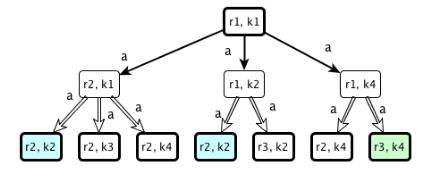
\includegraphics[scale = 0.6]{img/alb1.jpg}
  \end{figure}
\end{esempio}
\begin{esempio}
  Vediamo l'esempio di un gioco con due processi che dimostreremo non essere
  bisimili:\\

  Siano:
  \[q_1=a\cdot b\cdot Nil+a\cdot c\cdot Nil\]
  ovvero:
  \begin{center}
    \begin{tikzpicture}[shorten >=1pt,node distance=2cm,on grid,auto] 
      \node[state] (q_0) {$q_1$};  
      \node[state] (q_1) [below left =of q_0] {$q_2$};
      \node[state] (q_2) [below right =of q_0] {$q_3$};
      \node[state] (q_3) [below right =of q_1] {$Nil$};
      \path[->]
      (q_0) edge [above left] node {$a$} (q_1)
      (q_0) edge  node {$a$} (q_2)
      (q_1) edge [below left] node {$b$} (q_3)
      (q_2) edge  node {$c$} (q_3)
      ;
    \end{tikzpicture}
  \end{center}
 
  e:
  \[u_1=a\cdot (\tau\cdot b\cdot Nil+\tau\cdot c\cdot Nil)\]
  ovvero:
   \begin{center}
     \begin{tikzpicture}[shorten >=1pt,node distance=2cm,on grid,auto]
      
      \node[state] (q_0) {$u_2$};  
      \node[state] (q_1) [below left =of q_0] {$u_3$};
      \node[state] (q_2) [below right =of q_0] {$u_4$};
      \node[state] (q_3) [below right =of q_1] {$Nil$};
      \node[state] (q_4)[above =of q_0]  {$u_1$}; 
      \path[->]
      (q_0) edge [above left] node {$\tau$} (q_1)
      (q_0) edge  node {$\tau$} (q_2)
      (q_1) edge [below left] node {$b$} (q_3)
      (q_2) edge  node {$c$} (q_3)
      (q_4) edge  node {$a$} (q_0)
      ;
    \end{tikzpicture}
  \end{center}
  Vediamo quindi come si svolgono tutte le partite per $G(q_1,u_1)$.\\
  L'attaccante esegue $u_1\stackrel{a}{\rightarrow}u_2$.\\
  Il difensore ha due scelte:
  \begin{itemize}
    \item $q_1\stackrel{a}{\rightarrow}q_2$. Sono quindi in $(q_2,u_2)$. A
    questo punto $u_2\stackrel{\tau}{\rightarrow}u_4$ a cui il difensore non
    può che rispondere con l’azione nulla, $q_2\stackrel{\tau}{\rightarrow}q_2$,
    perdendo in quanto $q_2\not\approx^{Bis} u_4$ dato che dal primo, $q_2$
    posso fare solo $b$ e dal secondo, $u_4$ solo $c$ 
    
    
    \item $q_1\stackrel{a}{\rightarrow}q_3$. Sono quindi in $(q_3,u_2)$. A
    questo punto $u_2\stackrel{\tau}{\rightarrow}u_3$ a cui il difensore non
    può che rispondere con l’azione nulla, $q_3\stackrel{\tau}{\rightarrow}q_3$,
    perdendo in quanto $q_3\not\approx^{Bis} u_3$ dato che dal primo, $q_3$,
    posso fare solo $c$ e dal secondo, $u_3$, solo $b$
  \end{itemize}
  Quindi:
  \[q_1\not\approx^{Bis} u_1\]
  Vediamo anche in questo caso un albero parziale, dove si vedono anche le mosse
  in cui l'attaccante perdeva. Sono di egual colore le configurazioni identiche
  e si hanno col bordo bold le foglie (non colorate) corrispondi alle vincite
  del difensore, 
  che però non ha sempre una mossa per risponde attaccante, comportando la non
  bisimulazione:
  
  \begin{figure}[H]
    \centering
    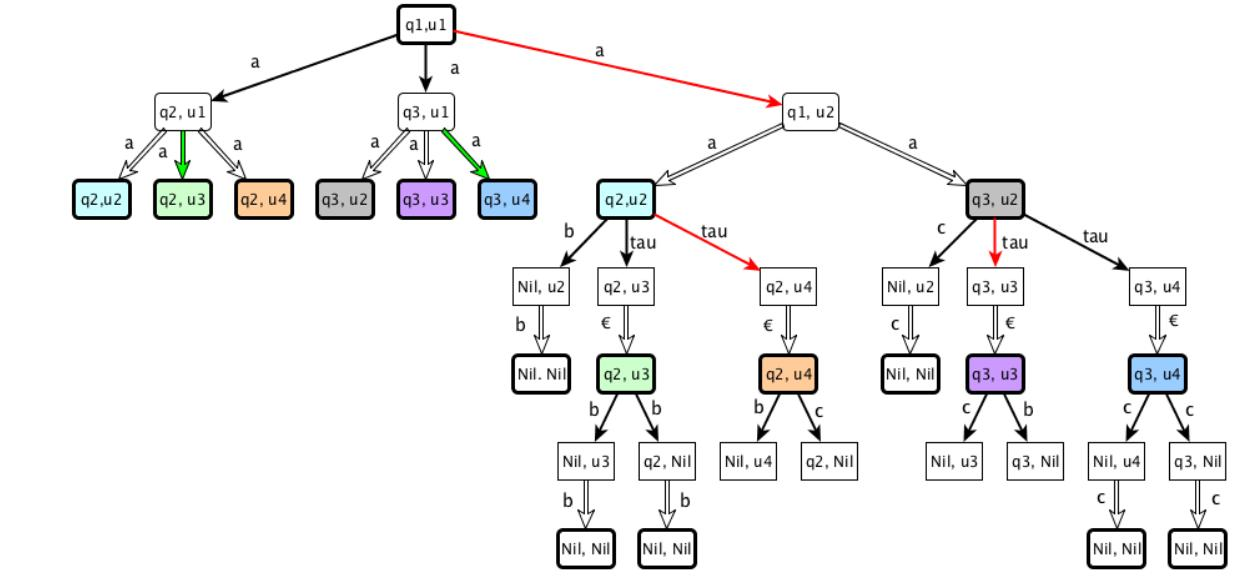
\includegraphics[scale = 0.31]{img/alb2.jpg}
  \end{figure}
  Si hanno infatti 4 foglie non colorate e non con il contorno bold che
  segnalano la vittoria dell'attaccante.\\
  Le foglie colorate rappresentano parti di alberi parziali.
\end{esempio}
\begin{itemize}
  \item se sono bisimili il difensore deve poter trovare una mossa vincente per
  ogni mossa dell'attaccante e quindi per ogni possibile mossa intermedia,
  avendo quindi una strategia vincente
  \item se non sono bisimili si ha almeno una mossa dell'attaccante, in ogni
  configurazione, per cui, comunque scelga poi il difensore, l'attaccante avrà
  ancora una mossa vincente, avendo quindi una strategia vincente
\end{itemize}
\textit{Se non si vuole dimostrare la bisimilitudine ma la si vuole cercare da
  zero bisogna studiare tutte le possibili partite o, meglio, un insieme di
  partite che mi possa dimostrare quale dei due giocatori ha la
  \textbf{strategia vincente}.}\\
Facciamo un piccolo ``recap'' della situazione.
\begin{definizione}
  Definiamo una \textbf{proprietà di equivalenza} tra processi CCS:
  \[\backsimeq \,\,\subseteq  Proc_{CCS}\times  Proc_{CCS}\]
  Si ha che, dati $p,q\in Proc_{CCS}$:
  \[\mbox{se }LTS(p)=LTS(q)\mbox{ allora } p\backsimeq q\]
  (ovvero se i due LTS sono isomorfi)\\
  Vale per altri modelli di concorrenza oltre che a il CCS.\\
  Si stanno considerando solo le azioni e non gli stati (si hanno altri approcci
  che considerano gli stati).
\end{definizione}
\begin{teorema}
  Si ha che, dati $p,q\in Proc_{CCS}$:
  \[p\backsimeq q\implies Tracce(p)=tracce(q)\]
  Qui le stesse sequenze di azioni possono essere eseguite su entrambi i
  processi.  
\end{teorema}
\begin{teorema}
  Si ha che, dati $\forall p,q\in Proc_{CCS}$, qualora si abbia che $p\backsimeq
  q$, i due processi devono avere la stessa possibilità di generare deadlock
  nell'interazione con l'ambiente (ovvero l'insieme dei processi con cui $p$ e
  $q$ possono interagire). Quindi sostituendo $p$ con $q$, qualora il
  primo non avesse deadlock, posso dire che anche il secondo non avrà deadlock
  se questi sono equivalenti.
\end{teorema}
\begin{teorema}
  Si ha che $\backsimeq$ deve essere una \textbf{congruenza} rispetto agli
  operatori del CCS. Deve essere possibile sostituire un sottoprocesso con un
  suo equivalente senza modificare il comportamento complessivo del
  sistema. Sostituendo quindi un sottoprocesso con un suo equivalente il
  processo di partenza deve essere equivalente al nuovo processo ottenuto dopo
  la sostituzione, in qualsiasi contesto ci si trovi.
\end{teorema}
\begin{definizione}
  Definiamo l'\textbf{equivalenza rispetto alle tracce forte} $\sim^T$. Dati
  $\forall p,q\in Proc_{CCS}$:
  \[LTS(p)=LTS(q)\implies p\sim^T q\]
  Anche qui si estrae dagli stati, osservando solo le tracce, e si ha che:
  \[p\sim^T q\iff Tracce(p)=Tracce(q)\]
\end{definizione}
\begin{teorema}
  Si dimostra che l'equivalenza rispetto alle tracce forte è una
  \textbf{congruenza} rispetto agli operatori CCS.
\end{teorema}
\begin{teorema}
  La nozione di equivalenza rispetto alle tracce forte non garantisce di
  preservare il deadlock o l'assenza di deadlock nell'interazione con l'ambiente
  (come visto nell'esempio \ref{coffe}, dove l'equivalenza rispetto alle tracce
  forte non è sufficiente a garantire nulla rispetto al deadlock).
\end{teorema}
Partendo da quanto sopra si introduce quindi concetto di \textbf{bisimulazione
  forte} (equivalenza forte rispetto alla bisimulazione), introdotto da
Milner. Si ricorda che, $\forall p,q\in Proc_{CCS}$, 
astraendo dagli stati:
\begin{itemize}
  \item $LTS(p)=LTS(q)\implies p\sim^{Bis}q$
  
  \item $p\sim^{Bis}q\implies Tracce(p)=Tracce(q)$. In altri termini si ha che
  $p\sim^{Bis}q\implies p\sim^T q$ e quindi:
  \[\sim^{Bis}\subseteq \sim^T\]
  non posso avere processi bisimili che non abbiano le stesse tracce
  \item la bisimulazione forte preserva il deadlock o l'assenza di deadlock
  nell'interazione con l'ambiente
  \item la bisimulazione forte è una congruenza rispetto agli operatori del CCS
\end{itemize}
Si ha però che la bisimulazione forte è troppo restrittiva infatti, come anche
$\sim^T$, non astrae $\tau$, avendo, per esempio, che $a\cdot b\cdot
Nil\not\sim^{Bis} a\cdot \tau\cdot b\cdot Nil$. Non posso quindi confrontare
alcuna specifica con sincronizzazioni interne alle componenti di un processo,
rispetto alle azioni non osservabili.\\ 
Si è introdotta quindi la regola di \textbf{transizione debole},
$\stackrel{a}{\Rightarrow}$.\\ 
Si ha \textbf{l'equivalenza debole rispetto alle tracce}, $\approx^T$ è meno
restrittiva rispetto a quella forte infatti:
\[p\sim^T q\implies p\approx^T q\]
e quindi:
\[\sim^T \subseteq \approx^T\]
Quindi se due processi sono equivalenti fortemente rispetto alle tracce lo
saranno anche debolmente. L'equivalenza debole rispetto alle tracce ha quindi le
seguenti proprietà, astraendo dagli stati:
\begin{itemize}
  \item $LTS(p)=LTS(q)\implies p\approx^{T}q$
  \item l'equivalenza debole rispetto alle tracce è una congruenza rispetto
  agli operatori del CCS 
  \item l'equivalenza debole rispetto alle tracce non garantisce di
  preservare il deadlock o l'assenza di deadlock nell'interazione con l'ambiente
\end{itemize}
Passando alla \textbf{bisimulazione debole} (equivalenza debole rispetto alla
bisimulazione), $\approx^{Bis}$ si ha che è meno 
restrittiva rispetto a quella forte infatti:
\[p\sim^{Bis} q\implies p\approx^{Bis} q\]
e quindi:
\[\sim^{Bis} \subseteq \approx^{Bis}\]
Si ha quindi che la bisimulazione forte è più restrittiva ell’equivalenza
rispetto alle tracce forte ed egualmente la bisimulazione debole è più
restrittiva ell’equivalenza rispetto alle tracce debole:
\[p\sim^{Bis}q\implies p\sim^T q\mbox{ e }p\approx^{Bis}q\implies p\approx^Tq\]
quindi si ha che:
\[\sim^{Bis}\subseteq\sim^T \mbox{ e }\approx^{Bis}\subseteq\approx^T\]
Non si hanno rapporti ``misti'' tra forte e debole.\\

\begin{definizione}
  Dato $p\in Proc_{CCS}$ si ha che esso è un \textbf{processo deterministico}
  sse vale che:
  \[\forall x\in Act,\mbox{se } p\stackrel{x}{\rightarrow}p'\mbox{ e
    }p\stackrel{x}{\rightarrow}p''\mbox{ allora }p'=p''\]
  Quindi se posso passare a $p'$ o $p''$ con la stessa azione allora
  necessariamente questi due processi coincidono.
\end{definizione}
\begin{esempio}
  vediamo un esempio di $p$ \textbf{non deterministico}:
  \[p=x\cdot p'+x\cdot p''\]
\end{esempio}
\begin{teorema}
  Siano $p,q\in Proc_{CCS}$ \textbf{deterministici} e sia $p\sim^Tq$ (quindi
  anche $p\approx^Tq$) allora si ha che:
  \[p\sim^{Bis}q\]
  e quindi anche:
  \[p\approx^{Bis}q\]
\end{teorema}
Avere processi deterministici con le stesse tracce non assicura che i due
processi abbiano lo stesso LTS. Come esempio basta vedere un processo $p=a\cdot
b\cdot a\cdot b\cdot p$ e uno $q=a\cdot b\cdot q$, dove il primo ha due nodi in
più anche se sono deterministici con quindi equivalenza rispetto alle tracce e
forte bisimilitudine, essendo quindi equivalenti, per entrambe le equivalenza,
debolmente.\\ 
Se ho invece due processi non entrambi deterministici potrei avere equivalenza
rispetto alle tracce (debole e forte) ma non bisimilitudine. Come esempio si
prendano $p=a\cdot \tau\cdot b\cdot Nil$ e $q=a\cdot(\tau\cdot b\cdot Nil+\tau
\cdot Nil)$, con quest'ultimo che non è un processo deterministico.\\
Basta quindi che un processo sia non deterministico per impedire il ``collasso''
dell'equivalenza rispetto alle tracce su quella rispetto alla bisimulazione.\\
Approfondiamo ora le proprietà della bisimulazione debole, tra cui:
\begin{itemize}
  \item la bisimulazione debole, per come è definita (unione di tutte le
  relazioni di bisimulazione), è la più grande relazione di bisimulazione debole
  ed è di equivalenza, essendo:
  \begin{itemize}
    \item riflessiva
    \item simmetrica
    \item transitiva
  \end{itemize}
  \item la bisimulazione debole, come quella forte, preserva la possibilità di
  generare o meno deadlock nell'interazione con l'ambiente, quindi sostituendo
  un processo che non genera deadlock con un suo bisimile ho che anche il nuovo
  sistema non andrà in deadlock (se invece generava un deadlock ora andrà
  in deadlock). Questa cosa, si ricorda, non è vera per le l'equivalenza sulle
  tracce
  
  \item la bisimulazione debole, a differenza di quella forte, astrae da azioni
  non osservabili, le $\tau$, e da cicli inosservabili, i $\tau$ loop. Se ho un
  ciclo infinito di $\tau$ si parla di \textbf{divergenza}.
  \begin{esempio}
    Presi un processo $Nil$ e uno $p=\tau\cdot p$ (quindi un processo infinito
    di sole $\tau$, una divergenza) ho che:
    \[Nil\approx^{Bis}p\]
    avendo:
    \begin{center}
      \begin{tikzpicture}[shorten >=1pt,node distance=2cm,on grid,auto] 
        \node[state] (q_0) {$p$};  
        \node[state] (q_3) [left =of q_0] {$Nil$};
        \path[->]
        (q_0) edge [loop right] node {$\tau$} (q_0)
        ;
      \end{tikzpicture}
    \end{center}
  \end{esempio}
  \begin{esempio}
    Siano $q=a\cdot b\cdot Nil$ e $s\cdot a\cdot v$ con $v=\tau\cdot v+b\cdot
    Nil$. Ho che:
    \[q\approx^{Bis} s\]
    ma:
    \[q\not\sim^{Bis} s\]

    avendo:
    \begin{center}
      \begin{tikzpicture}[shorten >=1pt,node distance=2cm,on grid,auto] 
        \node[state] (q_0) {$q$};  
        \node[state] (q_1) [right =of q_0] {$b\cdot Nil$};
        \node[state] (q_2) [right =of q_1] {$Nil$};
        \path[->]
        (q_0) edge  node {$a$} (q_1)
        (q_1) edge node {$b$} (q_2)
        ;
      \end{tikzpicture}
    \end{center}
    e
    \begin{center}
      \begin{tikzpicture}[shorten >=1pt,node distance=2cm,on grid,auto] 
        \node[state] (q_0) {$s$};  
        \node[state] (q_1) [right =of q_0] {$v$};
        \node[state] (q_2) [right =of q_1] {$Nil$};
        \path[->]
        (q_0) edge  node {$a$} (q_1)
        (q_1) edge node {$b$} (q_2)
        (q_1) edge [loop above] node {$\tau$} (q_1)
        ;
      \end{tikzpicture}
    \end{center}
  \end{esempio}
  \begin{esempio}
    Presi $q=a\cdot b\cdot Nil$, $r=a\cdot(\tau\cdot p+b\cdot Nil)$ e $s\cdot
    a\cdot v$ con $v=\tau\cdot v+b\cdot 
    Nil$. Ho che:
    \[q\not\approx^{Bis}r\]
    \[s\not\approx^{Bis}r\]
    \newpage
    avendo, oltre ai due LTS dell'esercizio precedente:
    \begin{center}
      \begin{tikzpicture}[shorten >=1pt,node distance=3cm,on grid,auto] 
        \node[state] (q_0) {$r$};  
        \node[state] (q_1) [right =of q_0] {$\tau\cdot p+b\cdot Nil$};
        \node[state] (q_2) [right =of q_1] {$Nil$};
        \node[state] (q_3) [above =of q_1] {$p$};
        \path[->]
        (q_0) edge  node {$a$} (q_1)
        (q_1) edge node {$b$} (q_2)
        (q_1) edge node {$\tau$} (q_3)
        (q_3) edge [loop above] node {$\tau$} (q_3)
        ;
      \end{tikzpicture}
    \end{center}
  \end{esempio}
\end{itemize}
Ci si chiede quindi se la bisimulazione debole sia o meno una congruenza
rispetto agli operatori del CCS.\\
Si ricorda che:
\begin{definizione}
  Data una relazione di equivalenza $R\subseteq Proc_{CCS}\times Proc_{CCS}$
  essa è una congruenza se $\forall C[\cdot]$, contesto CCS con una certa
  variabile non specificata ``$\cdot$'', presi $p,q\in Proc_{CCS}$, ho che:
  \[pRq\implies C[p]\,\,R\,\,C[q]\]
  Quindi comunque prendo una specifica CCS posso sostituire a piacere i due
  processi. 
\end{definizione}
\begin{teorema}
  Si ha che $\forall\,p,q\in Proc_{CCS}$ se $p\approx^{Bis}q$, allora:
  \begin{itemize}
    \item $a\cdot p\approx^{Bis} a\cdot q,\forall\, a\in
    Act=A\cup\overline{A}\cup\{\tau\}$ 
    \item $p|r\approx^{Bis}q|r\,\,\,\land \,\,\,
    r|p\approx^{Bis}r|q,\forall\,r\in Proc_{CCS}$  
    \item $p[f]\approx^{Bis}q[f],\forall\,f\mbox{ funzione di rietichettatura}$,
    ricordando che la funzione preserva nomi, co-nomi (quindi l'immagine di un
    co-nome è uguale al co-nome dell'immagine) e $\tau$
    \item $p_{\backslash L}\approx^{Bis}q_{\backslash L},\forall\,L\subseteq A$,
    ricordando che la restrizione rispetto a $L$ comporta che il processo può
    eseguire le azioni in $L$ solo se sono sincronizzazioni interne
  \end{itemize}
\end{teorema}
Si nota che nel teorema precedente abbiamo, in ordine:
\begin{itemize}
  \item prefisso
  \item composizione parallela
  \item rietichettatura
  \item restrizione
\end{itemize}
Non si parla quindi dell'operatore di scelta ``+'' che infatti necessita di
ulteriori approfondimenti. Vediamo un esempio:
\begin{esempio}
  Possiamo, per esempio, dire che:
  \[\tau\cdot a\cdot Nil\approx^{Bis}a\cdot Nil\]
  ma:
  \[\tau\cdot a\cdot Nil+b\cdot Nil\not\approx^{Bis}a\cdot Nil+b\cdot Nil\]
  graficamente si ha, per il primo:
  \begin{center}
    \begin{tikzpicture}[shorten >=1pt,node distance=3cm,on grid,auto] 
      \node[state] (q_0) {$p$};  
      \node[state] (q_1) [right =of q_0] {$a\cdot Nil$};
      \node[state] (q_2) [right =of q_1] {$Nil$};
      \path[->]
      (q_0) edge  node {$\tau$} (q_1)
      (q_1) edge node {$a$} (q_2)
      ;
    \end{tikzpicture}
  \end{center}
  e:
  \begin{center}
    \begin{tikzpicture}[shorten >=1pt,node distance=3cm,on grid,auto] 
      \node[state] (q_0) {$q$};  
      \node[state] (q_2) [right =of q_0] {$Nil$};
      \path[->]
      (q_0) edge  node {$a$} (q_2)
      ;
    \end{tikzpicture}
  \end{center}
  ma componendo $r=b\cdot Nil$ ottengo:
  \begin{center}
    \begin{tikzpicture}[shorten >=1pt,node distance=3cm,on grid,auto] 
      \node[state] (q_0) {$p+r$};  
      \node[state] (q_1) [right =of q_0] {$a\cdot Nil$};
      \node[state] (q_2) [right =of q_1] {$Nil$};
      \path[->]
      (q_0) edge  node {$\tau$} (q_1)
      (q_1) edge node {$a$} (q_2)
      (q_0) edge [bend left=45]  node {$b$} (q_2)
      ;
    \end{tikzpicture}
  \end{center}
  e:
  \begin{center}
    \begin{tikzpicture}[shorten >=1pt,node distance=3cm,on grid,auto] 
      \node[state] (q_0) {$q+r$};  
      \node[state] (q_2) [right =of q_0] {$Nil$};
      \path[->]
      (q_0) edge [bend left]  node {$a$} (q_2)
      (q_0) edge [bend right]  node [below] {$b$} (q_2)
      ;
    \end{tikzpicture}
  \end{center}
  vedendo che non sono bisimili perché $a\cdot Nil$ non può avere corrispondenti
  nel secondo LTS.
\end{esempio}
Si ha quindi che la \textbf{bisimulazione debole non è una congruenza per il
  CCS}, a differenza di quella forte (secondo la quale, nell'esempio precedente,
avremmo avuto direttamente $p\not\sim^{Bis}q$), in quanto non è una congruenza
rispetto alla scelta.\\
Si ha inoltre che la bisimulazione debole non è una congruenza rispetto alla
\textbf{ricorsione} (anche se non dimostriamo la cosa).\\
Possiamo quindi dire che la \textbf{bisimulazione debole è una congruenza
  rispetto agli operatori del CCS diversi da scelta e ricorsione.}\\
Vogliamo quindi identificare una relazione di congruenza, che è sempre una
relazione binaria tra processi CCS, che sia la più grande relazione contenuta
nella bisimulazione che sia però una congruenza rispetto a tutti gli
operatori:
\[\approx^C\subseteq\approx^{Bis}\subseteq Proc_{CCS}\times Proc_{CCS}\]
Per il CCS puro senza ricorsione Milner ha introdotto un insieme
finito di assiomi che possono essere visti come regole di riscrittura che
preservano la \textbf{congruenza all'osservazione}, che è la più grande
congruenza contenuta nella bisimulazione. Questo insieme di assiomi è quindi un
insieme finito per il quale, presi due processi $p,q\in Proc_{CCS}$, se riesco,
tramite questi assiomi, a trasformare l'uno nell'altro allora si ha che questi
processi non sono solo bisimili ma anche congruenti (potendo quindi sostituire
l'uno con l'altro in qualsiasi contesto che non includa la ricorsione). Questo
insieme di assiomi, detto $Ax$, è:
\begin{itemize}
  \item \textbf{corretto}, ovvero che se usando l'insieme di assiomi deduco che
  $p=q$ allora $p$ è congruente a $q$ rispetto a questa nuova nozione si
  congruenza:
  \[Ax\vdash p=q\implies p\approx^C q\]
  \item \textbf{completo}, ovvero presi due processi che sono congruenti secondo
  questa nuova nozione di congruenza allora sicuramente questo insieme di
  assiomi è completo in quanto mi permette, tale insieme, di trascrivere $p$ in
  $q$, ovvero:
  \[p\approx^C q\implies AX\vdash p=q\]
\end{itemize}
Vediamo quindi questi assiomi:
\begin{itemize}
  \item $p+(q+r)\approx^C (p+q)+r$ e $p|(q|r)\approx^C (p|q)|r$, ovvero
  l'assioma riguardo l'associatività di scelta e composizione parallela
  \item $p+q\approx^C q+p$ e $p|q\approx^Cq|p$, ovvero
  l'assioma riguardo la commutatività di scelta e composizione parallela
  \item $p+p\approx^C p$ ma $p|p\not\approx^C p$, ovvero si ha l'assioma per
  l'assorbimento riguardo la scelta ma non si ha riguardo la composizione
  parallela (si pensi per esempio a $p=\cdot Nil$ avrei $a$ due volte mentre $p$
  può fare $a$ una volta sola)  
  \item $p+Nil\approx^C p$ e $p|Nil \approx^Cp$, ovvero ovvero si ha l'assioma
  per l'assorbimento del $Nil$ riguardo la scelta e la composizione parallela
  \item $p+\tau\cdot p\approx^C\tau\cdot p$, che è l'assioma che risolve il
  problema di avere una scelta con un una $\tau$ iniziale nella sequenza, che
  non può essere eliminata
  \item $\mu\cdot \tau\cdot p\approx \mu\cdot p,\,\,\,\forall\,\mu\in Act$, che
  tratta le $\tau$ interne alla sequenza, che può essere eliminata
  \item $\mu\cdot(p+\tau\cdot 1)\approx^C\mu\cdot(p+\tau\cdot q)+\mu\cdot q$,
  ovvero per questo assioma si ha che il primo che è una ``semplificazione''
  del secondo (intuizione da esempio)
\end{itemize}
\begin{esempio}
  Vediamo l'ultimo assioma con un esempio.\\
  Siano:
  \[r_1=a\cdot(b\cdot Nil+\tau\cdot c\cdot Nil)\]
  \[k_1=a\cdot(b\cdot Nil+\tau\cdot c\cdot Nil)+a\cdot c\cdot Nil\]
  ovvero:
  \begin{center}
    \begin{tikzpicture}[shorten >=1pt,node distance=2cm,on grid,auto] 
      \node[state] (q_0) {$r_1$};  
      \node[state] (q_1) [right =of q_0] {$r_2$};
      \node[state] (q_2) [right =of q_1] {$Nil$};
      \node[state] (q_3) [above =of q_1] {$r_3$};
      \path[->]
      (q_0) edge  node {$a$} (q_1)
      (q_1) edge node {$b$} (q_2)
      (q_1) edge node {$\tau$} (q_3)
      (q_3) edge node {$c$} (q_2)
      ;
    \end{tikzpicture}
  \end{center}
  \newpage
  e:
  \begin{center}
    \begin{tikzpicture}[shorten >=1pt,node distance=2.5cm,on grid,auto] 
      \node[state] (q_0) {$k_1$};  
      \node[state] (q_1) [above right =of q_0] {$k_4$};
      \node[state] (q_2) [below right =of q_0] {$k_2$};
      \node[state] (q_3) [right=of q_2] {$k_3$};
      \node[state] (q_4) [above right=of q_2] {$Nil$};
      \path[->]
      (q_0) edge  node {$a$} (q_1)
      (q_0) edge  node {$a$} (q_2)
      (q_2) edge node {$b$} (q_3)
      (q_2) edge node {$\tau$} (q_4)
      (q_1) edge node {$c$} (q_4)
      (q_3) edge node {$c$} (q_4)
      ;
    \end{tikzpicture}
  \end{center}
  e si ha vede che:
  \[r_1\approx^C k_1\]
  con il primo che è una ``semplificazione'' del secondo.
\end{esempio}
Si hanno anche altri assiomi legati al fatto che $p$ e $q$ siano delle somme,
ovvero:
\[p=\sum_i a_i\cdot p_i,\,\,\,a\in Act\]
\[q=\sum_j b_j\cdot q_j,\,\,\,b\in Act\]
avendo quindi i seguenti assiomi:
\begin{itemize}
  \item $p|q\approx^C\sum_i a_i\cdot (p_i|q)+\sum_j b_j\cdot
  (p|q_j)+\sum_{a_i=\overline{b_j}}\tau\cdot(p_i|q_j)$ che è l'assioma detto
  \textbf{teorema di espansione di Milner} (nell'ultima parte ho che se $a_i$ e
  $b_j$ sono l'uno il complemento dell'altro allora posso sincronizzare su di
  essi i processi, che diventano una $\tau$ e proseguendo con $p_i|q_j$). È la
  generalizzazione dell'operatore parallelo con la regola d'inferenza vista ad
  inizio capitolo.
  \item $p[f]\approx^C \sum_if(a_i)\cdot(p_i[f]),\,\,\,\forall\,f\mbox{ funzione
    di etichettatura}$, ovvero etichettare tutto il processo $p$ corrisponde al
  fatto di ottenere congruo il processo che ottengo etichettando ogni i-sima
  azione delle componenti che sono in alternativa con il processo relativo
  rietichettato con $f$
  \item $p_{\backslash L}\approx^C \sum_{a_i,\overline{a_i}\not\in
    L}a_i\cdot(p_{i\backslash L}),\,\,\,\forall\,L\subseteq A$ quindi considero
  solo le azioni per le quali non si ha al restrizione
\end{itemize}
Per cui la bisimulazione risulta tale per cui se usiamo $\approx^C$ si può
modellare un sistema a passi successivi sapendo che posso sostituire un
sottoprocesso con un altro ottenendo ancora un sistema bisimile al precedente.
\begin{esempio}
  Vediamo un esempio sull'assioma detto \textbf{teorema di espansione}.\\
  Si ha, sviluppando a partire dal primo:
  \[a\cdot c\cdot Nil|b\cdot Nil\approx^C\]
  \[a\cdot(c\cdot NIl|b\cdot Nil)+b\cdot(a\cdot c \cdot Nil|Nil)\approx^C\]

  \[a\cdot(c\cdot(Nil|b\cdot Nil)+b\cdot(c\cdot Nil|Nil))+b\cdot(a\cdot(c\cdot
    Nil|Nil))\approx^C\]
  \[a\cdot (c\cdot b\cdot(NIl|Nil)+b\cdot c\cdot(Nil|NIl))+b\cdot(a\cdot
    c\cdot(Nil|Nil))\approx^C\]
  \[a\cdot(c\cdot b\cdot Nil+b\cdot c\cdot Nil)+b\cdot a\cdot c\cdot Nil\]
  e quindi:
  \[a\cdot c\cdot Nil|b\cdot Nil\approx^Ca\cdot(c\cdot b\cdot Nil+b\cdot c\cdot
    Nil)+b\cdot a\cdot c\cdot Nil\]
  infatti si ha:
   \begin{center}
    \begin{tikzpicture}[shorten >=1pt,node distance=4cm,on grid,auto] 
      \node[elliptic state] (q_0) {$a\cdot c\cdot Nil |b\cdot Nil$};  
      \node[elliptic state] (q_1) [below left =of q_0] {$c\cdot Nil|b\cdot Nil$};
      \node[elliptic state] (q_2) [below right =of q_0] {$a\cdot c\cdot Nil|Nil$};
      \node[elliptic state] (q_3) [below left=of q_2] {$c\cdot Nil|Nil$};
      \node[elliptic state] (q_4) [below=of q_1] {$Nil|b\cdot Nil$};
      \node[elliptic state] (q_5) [below right=of q_4] {$Nil$};
      \path[->]
      (q_0) edge [above left] node {$a$} (q_1)
      (q_0) edge  node {$b$} (q_2)
      (q_1) edge [below left]node {$b$} (q_3)
      (q_1) edge node {$c$} (q_4)
      (q_2) edge node {$a$} (q_3)
      (q_3) edge node {$c$} (q_5)
      (q_4) edge node {$b$} (q_5)
      ;
    \end{tikzpicture}
  \end{center}
\end{esempio}
\begin{esempio}
  Vediamo l'esempio della \textbf{mutua esclusione} con la primitiva di un
  \textbf{semaforo}. \\
  Si ha la specifica:
  \[spec=b_1\cdot e_1\cdot spec+b_2\cdot e_2\cdot spec\]
  \begin{center}
    \begin{tikzpicture}[shorten >=1pt,node distance=3cm,on grid,auto] 
      \node[elliptic state] (q_0) {$spec$};  
      \node[elliptic state] (q_1) [below left =of q_0] {$e_1\cdot spec$};
      \node[elliptic state] (q_2) [below right =of q_0] {$e_2\cdot spec$};
      \path[->]
      (q_0) edge [bend right = 25] node [above left]{$b_1$} (q_1)
      (q_0) edge [bend left= 25] node {$b_2$} (q_2)
      (q_1) edge [bend right = 25] node [below right] {$e_1$} (q_0)
      (q_2) edge [bend left= 25] node {$e_2$} (q_0)
      ;
    \end{tikzpicture}
  \end{center}
  e l'implementazione:
  \[sys=(A_1|S|A_2)_{\backslash\{p,v\}}\]

  con:
  \[S=p\cdot v\cdot S\]
  \begin{center}
    \begin{tikzpicture}[shorten >=1pt,node distance=2cm,on grid,auto] 
      \node[state] (q_0) {$S$};  
      \node[state] (q_1) [below =of q_0] {$v\cdot S$};
      \path[->]
      (q_0) edge [bend right = 25] node [above left]{$p$} (q_1)

      (q_1) edge [bend right = 25] node [below right] {$v$} (q_0)
      ;
    \end{tikzpicture}
  \end{center}
  e con:
  \[A_1=\overline{p}\cdot b_2\cdot e_1\cdot \overline{v}\cdot A_1\]
  \[A_2=\overline{p}\cdot b_2\cdot e_2\cdot \overline{v}\cdot A_2\]
  \begin{center}
    \begin{tikzpicture}[shorten >=1pt,node distance=2cm,on grid,auto] 
      \node[elliptic state] (q_0) {$A_1$};  
      \node[elliptic state] (q_1) [below =of q_0] {$b_i\cdot
        e_i\cdot\overline{v}\cdot A_i$}; 
      \node[elliptic state] (q_2) [below =of q_1] {$e_i\cdot \overline{v}\cdot
        A_i$}; 
      \node[elliptic state](q_3) [below =of q_2] {$\overline{v}\cdot A_i$};
      \path[->]
      (q_0) edge node {$\overline{p}$} (q_1)
      (q_1) edge node {$b_i$} (q_2)
      (q_2) edge node {$e_i$} (q_3)
      (q_3) edge [bend right = 65]node [right]{$\overline{v}$} (q_0)
      ;
    \end{tikzpicture}
  \end{center}
  Si ha quindi:
  \begin{center}
    \begin{tikzpicture}[shorten >=1pt,node distance=5cm,on grid,auto] 
      \node (q_0) {$(A_1|S|A_2)_{\backslash\{p,v\}}$};  
      \node (q_1) [below left =of q_0] {$(b_1\cdot e_1\cdot \overline{v}\cdot
        A_1|v\cdot S|A_2)_{\backslash\{p,v\}}$};
      \node (q_2) [below right =of q_0] {$(A_1|v\cdot S|b_2\cdot e_2\cdot
        \overline{v}\cdot A_2)_{\backslash\{p,v\}}$};
      \node (q_3) [below =of q_1] {$(e_1\cdot \overline{v}\cdot
        A_1|v\cdot S|A_2)_{\backslash\{p,v\}}$};
      \node (q_4) [below =of q_3] {$\overline{v}\cdot
        A_1|v\cdot S|A_2)_{\backslash\{p,v\}}$};
      \node (q_5) [below =of q_2] {$(A_1|v\cdot S| e_2\cdot
        \overline{v}\cdot A_2)_{\backslash\{p,v\}}$};
      \node (q_6) [below =of q_5] {$(\overline{v}\cdot A_2)_{\backslash\{p,v\}}$};
      \path[->]
      (q_0) edge node [above left] {$\tau$} (q_1)
      (q_0) edge node {$\tau$} (q_2)
      (q_1) edge node {$b_1$} (q_3)
      (q_3) edge node {$e_1$} (q_4)
      (q_2) edge node {$b_2$} (q_5)
      (q_5) edge node {$e_2$} (q_6)
      (q_6) edge [bend left = 20] node [above right]{$\tau$} (q_0)
      (q_4) edge [bend right = 20] node {$\tau$} (q_0)
      ;
    \end{tikzpicture}
  \end{center}
  Vedo se $spec\approx^{Bis}sys$ ma ho che l'attaccante ha una strategia
  vincente, fa una $\tau$ sul primo processo in $sys$. Nella seconda mossa poi
  l'attaccante opera su $spec$ facendo $b_2$ e il difensore perde:
  \[spec\not\approx^{Bis}sys\]
\end{esempio}
\textbf{altri esempi su slide.}\\
Dati due processi $p_1$ e $p_2$ abbiamo che la composizione parallela è detta a
\textbf{semantica interleaving}, in quanto si vede dalle regole di inferenza che
posso eseguire o uno o l'altro o sincronizzare, grazie all'assunzione
dell'atomicità delle azioni
La cosa è visibile per esempio con:
\[p=a\cdot Nil|b\cdot Nil\]
\[q=a\cdot b\cdot Nil+b\cdot a\cdot Nil\]
Avendo:
\[p\sim^{Bis}q\]
Togliendo l'atomicità, mettendo $a$ come $a_1,a_2$ si ha:
\[p'=p_{\left[a \leftarrow a_{1} \cdot a_{2}\right]}=a_{1} \cdot a_{2}
  \cdot N i l \mid b . N i l \]
\[      q'=q_{\left[a \leftarrow a_{1}, a_{2}\right]}=a_{1} \cdot a_{2}
  \cdot b \cdot N i l+b \cdot a_{1} \cdot a_{2} \cdot N i l\]
Avendo:
\begin{center}
  \begin{tikzpicture}[shorten >=1pt,node distance=3cm,on grid,auto] 
    \node[elliptic state] (q_0) {$p'$};  
    \node[elliptic state] (q_1) [below left =of q_0] {$a_2\cdot Nil|b\cdot
      Nil$};
    
    \node[elliptic state] (q_2) [below right =of q_0] {$a_1\cdot a_2\cdot
      Nil|Nil$};
    
    \node[elliptic state] (q_3) [below left=of q_2] {$a_2\cdot Nil|Nil$};
    \node[elliptic state] (q_4) [below=of q_1] {$Nil|b\cdot Nil$};
    \node[elliptic state] (q_5) [below right=of q_4] {$Nil| Nil$};
    \path[->]
    (q_0) edge [above left] node {$a_1$} (q_1)
    (q_0) edge  node {$b$} (q_2)
    (q_1) edge [below left]node {$b$} (q_3)
    (q_1) edge node {$a_2$} (q_4)
    (q_2) edge node {$a_1$} (q_3)
    (q_3) edge node {$a_2$} (q_5)
    (q_4) edge node {$b$} (q_5)
    ;
  \end{tikzpicture}
\end{center}
\newpage
e:
\begin{center}
  \begin{tikzpicture}[shorten >=1pt,node distance=3cm,on grid,auto] 
    \node[elliptic state] (q_0) {$p'$};  
    \node[elliptic state] (q_1) [below left =of q_0] {$a_2\cdot b\cdot
      Nil$};
    
    \node[elliptic state] (q_2) [below right =of q_0] {$a_1\cdot a_2\cdot
      Nil$};
    
    \node[elliptic state] (q_3) [below =of q_2] {$a_2\cdot Nil$};
    \node[elliptic state] (q_4) [below=of q_1] {$b\cdot Nil$};
    \node[elliptic state] (q_5) [below right=of q_4] {$Nil$};
    \path[->]
    (q_0) edge [above left] node {$a_1$} (q_1)
    (q_0) edge  node {$b$} (q_2)
    (q_1) edge node {$a_2$} (q_4)
    (q_2) edge node {$a_1$} (q_3)
    (q_3) edge node [above left] {$a_2$} (q_5)
    (q_4) edge node {$b$} (q_5)
    ;
  \end{tikzpicture}
\end{center}
e si ha che $p'\neq\sim^Tq'$. Se le azioni non sono più atomiche quindi
``rompo'' la composizione parallela, avrei bisogno infatti di una semantica
basata sulla \textbf{true concurrency}.\\
Nella letteratura è stata definita la bisimulazione definita differenziando
azioni concorrenti e in sequenza (per esempio tramite le reti di Petri, che si
basano sulla \textit{true concurrency}).\\
\textbf{Sulle slide esempio di un protocollo di comunicazione fatto con CCS e
  poi con reti di Petri e ulteriori esempi di partite per la bisimulazione}.
\chapter{Reti di Petri}
% \begin{center}
%   \begin{tikzpicture}[node distance=2cm,bend angle=45,auto]

%     \node [transition] (t) [below right of = py, label=right:$t$] {};
%     \node [place] (p1) [above of = t, label=right:$$] {$p_1$};
%     \node [place] (p2) [below of = t, label=right:$$] {$p_2$};
%     \path[-{Latex[width=2mm]}]
%     (p1) edge (t)
%     (t) edge (p2)

%   \end{tikzpicture}
% \end{center}
Abbiamo introdotto un'algebra di processi come CCS dove processi sequenziali
interagiscono tra loro tramite handshaking. Un altro modello usato, con varie
implementazioni, sono gli automi a stati finiti (usati per reti neurali,
riconoscitori di linguaggi, modelli di protocolli di comunicazioni
etc$\ldots$).\\
Si passa ora alle \textbf{reti di Petri}, introdotte da Petri nel 1962 nella sua
tesi di dottorato, partendo da una critica ai modelli fatti tramite automi a
stati per protocolli di comunicazioni.\\

La nuova teoria dei sistemi è basata sui principi della fisica quantistica, il
modello, nell’ottica di Petri, non è quindi un modello chiuso ma è 
in grado di \textbf{comunicare con l’ambiente} (in sintonia con le teorie della
fisica). Vuole una teoria dei sistemi in grado di descrivere il flusso di
informazioni e che permetta di analizzare sistemi con un'organizzazione
complessa.\\
La sua teoria generale dei sistemi che processano informazione si basa su, tra
le altre cose:
\begin{itemize}
  \item comunicazione
  \item sincronizzazione
  \item flusso di informazione
  \item relazione di concorrenza e indipendenza causale
\end{itemize}
A partire dagli anni '70 questa teoria si è sviluppata dal punto di vista
dell'espressività, portando allo studio di diverse classi di reti. Si sviluppano
anche tecniche formali di analisi e di verifica delle reti (tramite algebra
lineare, teoria dei grafi etc$\ldots$). Le reti di Petri hanno tantissimi ambiti
d'uso, tra i quali:
\begin{itemize}
  \item specificare protocolli di comunicazione
  \item disegnare circuiti asincroni
  \item algoritmi concorrenti/paralleli
  \item modellare sistemi organizzativi
  \item modellare db distribuiti
  \item specificare sistemi di controllo industriali
  \item modellare sistemi biologici e per modellare reazioni chimiche
  \item valutare le prestazioni (tramite reti stocastiche e temporizzate)
\end{itemize}
\begin{definizione}
  I \textbf{sistemi di transizione etichettati} sono definiti come gli automi a
  stati finiti ma senza essere visti come riconoscitori di linguaggi infatti un
  sistema è formato da un insieme, solitamente finito, di stati globali $S$. Si
  ha poi un \textit{alfabeto} delle possibili azioni che può eseguire il
  sistema. Si hanno anche delle relazioni di transizioni, ovvero delle
  transizioni che permettono di specificare come, attraverso un'azione, si passa
  da uno stato ad un altro. Le transizioni si rappresentano con archi
  etichettati tra i nodi, che rappresentano 
  gli stati. Le etichette degli archi rappresentano le azioni necessarie alla
  trasformazione. L'insieme delle azioni viene chiamato $E$ mentre $T\subseteq
  S\times E\times S$ è l'insieme degli archi etichettati. Può essere,
  opzionalmente, individuato uno stato iniziale $s_0$. Un sistema non è
  obbligato a ``terminare'', quindi non si ha obbligatoriamente uno stato
  finale.\\ 
  Riassumendo quindi un sistema di transizione etichettato è un quadrupla:
  \[A=(S,E,T,s_0)\]
  % aggiungere pic
  % \begin{figure}[H]
  %   \centering
  %   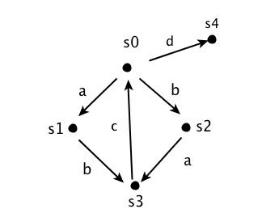
\includegraphics[scale = 0.5]{img/ste.jpg}
  %   \caption{Esempio di sistema di transizione etichettato}
  % \end{figure}
\end{definizione}
La critica di Petri è che in un sistema distribuito non sia individuabile uno
\textbf{stato globale}, che in un sistema distribuito le trasformazioni di stato
siano \textbf{localizzate} e non globali, che non esista un sistema di
riferimento temporale unico (si possono avere più assi temporali in un sistema
distribuito). Quindi la simulazione sequenziale non deterministica (semantica a
``interleaving'') dei sistemi distribuiti è una forzatura e non rappresenta le
reali caratteristiche del comportamento del sistema, ovvero la località, la
distribuzione degli eventi e la relazione di dipendenza causale e non causale
tra gli eventi.
\section{Sistemi elementari}

Introduciamo quindi i \textbf{sistemi elementari}.\\
Per introdurre i sistemi elementari delle reti di Petri, ovvero una classe molto
semplice e astratta, partiamo da un esempio:
\begin{esempio}
  Vediamo l'esempio del \textit{Produttore e del Consumatore}.\\
  Si ha un sistema con una componente Produttore che produce elementi e li
  deposita in un buffer che ha un'unica posizione (quindi o è pieno o è vuoto) e
  con un consumatore che preleva dal buffer un elemento per poi consumarlo ed
  essere pronto a prelevare un altro elemento. Si ha un comportamento
  ciclico. Usiamo quindi le reti di Petri, col modello dei sistemi elementari,
  per rappresentare questo modello. Bisogna quindi individuare le proprietà
  fondamentali locali del sistema.\\
  Partiamo dal produttore, che può avere 2 stati locali:
  \begin{enumerate}
    \item pronto per produrre
    \item pronto per depositare
  \end{enumerate}
  Usiamo i \textbf{cerchi} per rappresentare condizioni locali che sono
  associabili a delle proposizioni della logica che possono essere vere o
  false. Queste preposizioni sono quindi stati locali. Gli eventi locali vengono
  invece rappresentati con un \textbf{rettangolo}. Un evento ha un arco entrante
  da uno stato che rappresenta le \textit{precondizioni} di quell'evento (che
  devono essere vere per permettere l'occorrenza dell'evento). L'occorrenza
  dell'evento rende false le precondizioni e rende vere le
  \textit{postcondizioni} (che sono stati raggiungibili con un arco uscente da
  un evento). Si ha quindi che il produttore può depositare solo se il buffer
  non è pieno, quindi le postcondizioni di un evento devono essere false
  affinché l'evento possa occorrere (oltre alle precondizioni vere).\\
  Passiamo al consumatore che estrae solo se il buffer è pieno ed è pronto a
  prelevare. Si procede poi con la stessa logica del produttore di cambiamento
  tra vero e falso delle varie condizioni locali.\\
  In questo esempio si hanno quindi condizioni che sono preposizioni booleane e
  rappresentano stati locali. Si ha quindi a sinistra il produttore, a destra il
  consumatore e in mezzo il buffer:
  \begin{center}
    \begin{tikzpicture}[node distance=2cm,bend angle=45,auto]
      \node [place] (p0) [label=above:pronto a depositare] {};
      \node [transition] (t1) [below right of = p0, label=left:deposita] {};
      \node [transition] (t2) [below left of = p0, label=left:produce] {};
      \node [place] (p1) [below right of = t2, label=below:pronto a produrre]
      {}; 
      \node [place] (p3) [right of = t1, label=above:buffer pieno] {};
      \node [transition] (t4) [right of = p3, label=right:estrae] {};

      \node [place] (p2) [above right of = t4,label=above:pronto a prelevare]
      {}; 
      \node [transition] (t3) [below right of = p2, label=right:consuma] {};
      \node [place] (p4) [below right of = t4, label=below:pronto a consumare]
      {}; 
      
      \path[-{Latex[width=2mm]}]
      (p0) edge (t1)
      (t1) edge (p1)
      (p1) edge (t2)
      (t2) edge (p0)
      (t1) edge (p3)
      (p3) edge (t4)
      (t4) edge (p4)
      (p4) edge (t3)
      (t3) edge (p2)
      (p2) edge (t4)
      ;
    \end{tikzpicture}
  \end{center}

  Lo stato globale del sistema è dato da una
  collezione di stati locali. Per segnare tali condizioni mettiamo un punto
  pieno dentro il cerchio e queste condizioni ``abilitano'' i vari eventi:
  \begin{center}
    \begin{tikzpicture}[node distance=2cm,bend angle=45,auto]
      \node [place] (p0) [label=above:pronto a depositare] {};
      \node [transition] (t1) [below right of = p0, label=left:deposita] {};
      \node [transition] (t2) [below left of = p0, label=left:produce] {};
      \node [place, tokens=1] (p1) [below right of = t2, label=below:pronto a
      produrre] {}; 
      \node [place] (p3) [right of = t1, label=above:buffer pieno] {};
      \node [transition] (t4) [right of = p3, label=right:estrae] {};

      \node [place, tokens=1] (p2) [above right of = t4,label=above:pronto a
      prelevare] {}; 
      \node [transition] (t3) [below right of = p2, label=right:consuma] {};
      \node [place] (p4) [below right of = t4, label=below:pronto a consumare]
      {}; 
      
      \path[-{Latex[width=2mm]}]
      (p0) edge (t1)
      (t1) edge (p1)
      (p1) edge (t2)
      (t2) edge (p0)
      (t1) edge (p3)
      (p3) edge (t4)
      (t4) edge (p4)
      (p4) edge (t3)
      (t3) edge (p2)
      (p2) edge (t4)
      ;
    \end{tikzpicture}
  \end{center}
  Si può arrivare ad una \textit{configurazione} dove, per esempio, sia l'evento
  \textit{produce}, del produttore, che l'evento \textit{preleva}, del
  consumatore, sono abilitati. Si ha quindi che i due eventi possono occorrere
  in modo \textbf{concorrente} infatti i due eventi sono \textbf{indipendenti}
  in quanto condizionati da \textbf{precondizioni e postcondizioni completamente
    disgiunte}. Due eventi che occorrono in maniera concorrente lo possono fare in
  qualsiasi ordine, non si ha infatti una sequenza temporale specifica tra i
  due. \\
  In questo sistema quindi siano solo stati locali ed eventi localizzati e non
  stati ed eventi globali. Un evento dipende solo dalle sue precondizioni e
  dalle sue postcondizioni.\\
  \textit{Se rappresentiamo con delle marche le condizioni vere possiamo
    simulare il comportamento del sistema con il \textit{gioco delle marche} che
    mostra come l'evoluzione delle condizioni avviene all'occorrenza degli
    eventi.} \\
  La simula di un tale sistema può comunque avvenire con un sistema di
  transizioni etichettato, ovvero con un automa a stati finiti, che rappresenta
  gli stati globali corrispondenti alle diverse combinazioni di stati locali che
  di volta in volta sono veri.
  \newpage
  Gli archi vengono etichettati con gli eventi che
  comportano un cambiamento di stato globale:
 \begin{center}
    \begin{tikzpicture}[node distance=2cm,bend angle=45,auto]
      \node [place] (p0) [label=above:P2] {};
      \node [transition] (t1) [below right of = p0, label=left:d] {};
      \node [transition] (t2) [below left of = p0, label=left:p] {};
      \node [place, tokens=1] (p1) [below right of = t2, label=below:P1] {}; 
      \node [place] (p3) [right of = t1, label=above:B] {};
      \node [transition] (t4) [right of = p3, label=right:e] {};

      \node [place, tokens=1] (p2) [above right of = t4,label=above:C1] {}; 
      \node [transition] (t3) [below right of = p2, label=right:c] {};
      \node [place] (p4) [below right of = t4, label=below:C2]
      {}; 
      
      \path[-{Latex[width=2mm]}]
      (p0) edge (t1)
      (t1) edge (p1)
      (p1) edge (t2)
      (t2) edge (p0)
      (t1) edge (p3)
      (p3) edge (t4)
      (t4) edge (p4)
      (p4) edge (t3)
      (t3) edge (p2)
      (p2) edge (t4)
      ;
    \end{tikzpicture}
  \end{center}
  \begin{figure}[H]
    \centering
    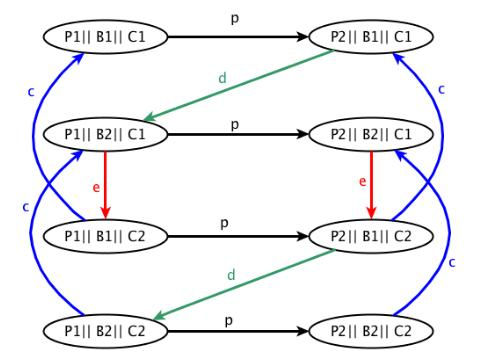
\includegraphics[scale = 0.6]{img/prod3.jpg}
    \caption{Rappresentazione del sistema con un automa a stati finiti che
      rappresenta stati globali}
  \end{figure}
  Lo stesso evento in algebra di processi sarebbe (espandendo il buffer $B$ in
  un modo che poi specificheremo per specificare pieno e vuoto):
  \[S=(P1|B1|C1)_{\{\backslash deposita, estae\}}\]
  \[P1=produce\cdot P2\]
  \[P2=\overline{deposita}\cdot P1\]
  \[C1=estrae\cdot C2\]
  \[C2=consuma\cdot C1\]
  \[B1=deposita\cdot B2\]
  \[B2=\overline{estae}\cdot B1\]
  \begin{figure}[H]
    \centering
    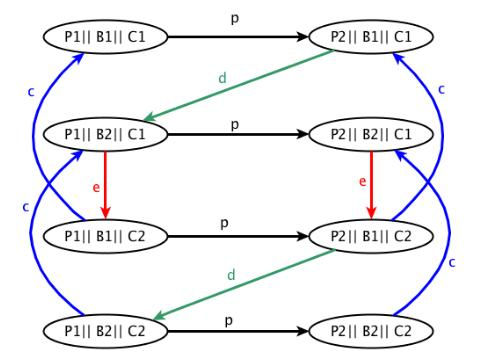
\includegraphics[scale = 0.6]{img/prod3.jpg}
    \caption{Rappresentazione del sistema con un automa a stati finiti che
      rappresenta stati globali}
  \end{figure}
\end{esempio}
Passiamo ora alla formalizzazione di questi aspetti.\\
\begin{definizione}
  Una \textbf{rete elementare} è definita come una tripla:
  \[N=(B,E,F)\]
  dove:
  \begin{itemize}
    \item $B$ è un insieme finito di \textbf{condizioni}, ovvero \textit{stati
      locali}, proprietà/proposizioni booleane etc$\ldots$. Vengono
    rappresentate con un cerchio 
    \item $E$ è un insieme finito di \textbf{eventi}, ovvero trasformazioni
    locali di stato e \textit{transizioni locali}. Vengono rappresentate con un
    quadrato o con un rettangolo pieno
    \item $F$ è una \textbf{relazione di flusso} che connette condizioni ad
    eventi ed eventi a condizioni. Si ha quindi che:
    \[F\subseteq (B\times E)\cup(E\times B)\]
    Le relazioni di flusso sono rappresentate da archi orientati. Inoltre la
    relazione di flusso è tale per cui non esistano \textbf{elementi isolati},
    in quanto non avrebbero senso, in un tale sistema, eventi isolati (che non
    modificherebbero mai una condizione) o condizioni isolate (che non
    verrebbero mai modificate da un evento). Si ha, formalmente, che: 
    \[dom(F)\cup ran(F)=B\cup E\]
    ovvero non ho condizioni/eventi isolati, in quanto non avrebbero senso
    (potrei anche non modellarle), avrei una condizione costante e un
    evento che non accade mai, quindi dominio e codominio di $F$ coprono
    l'insieme di condizioni ed eventi
  \end{itemize}
  Si ha che:
  \[B\cap E = \emptyset\]
  \[B\cup E \neq \emptyset\]
  Ovvero gli insiemi delle condizioni e degli eventi sono tra loro disgiunti e
  non vuoti.\\
  Sia ora $x$ un elemento qualsiasi della rete, ovvero $x$ può essere o una
  condizione o un evento, formalmente:
  \[x\in B\cup E\]
  Si ha che, dato $X=B\cup E$:
  \begin{itemize}
    \item $^\bullet x=\{y\in X:\,(y,x)\in F\}$ rappresenta l'insieme di tutti gli
    elementi $y$ che sono connessi dalla relazione di flusso ad $x$, ovvero si
    ha un arco da $y$ a $x$. Sono quindi i \textbf{pre-elementi} di $x$, ovvero
    le \textit{precondizioni}, se $x$ è un evento, o i \textit{pre-eventi}, se
    $x$ è una condizione
    \item $x^\bullet=\{y\in X:\,(x,y)\in F\}$ rappresenta l'insieme di tutti gli
    elementi $y$ che sono connessi dalla relazione di flusso a partire da $x$,
    ovvero si ha un arco da $x$ a $y$. Sono quindi i \textbf{post-elementi} di
    $x$, ovvero le \textit{postcondizioni}, se $x$ è un evento, o i
    \textit{post-eventi}, se $x$ è una condizione
  \end{itemize}
  Posso estendere questa notazione ad insiemi di elementi. Sia $A$ un insieme
  qualsiasi di elementi, che possono quindi essere sia condizioni che eventi:
  \[A\subseteq B\cup E\]
  Si ha quindi che i pre-elementi dell'insieme $A$ sono rappresentati con:
  \[^\bullet A=\cup_{x\in A}\, ^\bullet x\]
  ovvero l'unione dei pre-elementi di ogni singolo elemento dell'insieme $A$.\\
  Analogamente si ha che i post-elementi dell'insieme $A$ sono rappresentati
  con: 
  \[A^\bullet=\cup_{x\in A} x^\bullet\]
  ovvero l'unione dei post-elementi di ogni singolo elemento dell'insieme $A$.
  \textit{Nelle reti c'è sempre una relazione di \textbf{dualità} tra due
    elementi, per esempio tra condizioni ed eventi, tra pre-eventi e
    post-eventi, tra pre-condizioni e post-condizioni. Inoltre si ha la
    caratteristica della \textbf{località}, quindi si hanno stati locali e
    trasformazioni di stato locali} 
\end{definizione}
La rete $N=(B,E,F)$ descrive la \textit{struttura statica del sistema}, il
comportamento é definito attraverso le nozioni di \textbf{caso (o
  configurazione)} e di \textbf{regola di scatto (o di transizione)}.\\
Una rete può anche essere suddivisa in sotto-reti, seguendo l'esempio sopra si
potrebbe avere una sotto-rete per il produttore, una per il consumatore e anche
una per il buffer.\\
\begin{definizione}
  Un \textbf{caso} (o \textbf{configurazione}) é un insieme di condizioni
  $c\subseteq B$ che rappresentano l’insieme di condizioni vere in una certa
  configurazione del sistema, un insieme di \textbf{stati locali} che
  collettivamente individuano lo \textbf{stato globale} del sistema.\\
  Graficamente le condizioni vere presentano un puntino in mezzo al cerchio
  mentre le condizioni false solo un cerchio vuoto:
  \begin{center}
    \begin{tikzpicture}[node distance=2cm,bend angle=45,auto]
      \node [place] (p0) [label=above:False] {};
      \node [place, tokens=1] (p1) [right of = p0,label=above:True] {};
      {}; 
      
    \end{tikzpicture}
  \end{center}
\end{definizione}
\begin{definizione}
  Sia $N=(B,E,F)$ una rete elementare e sia $c\subseteq B$ una certa
  configurazione (non serve quindi necessariamente conoscere tutto lo stato del
  sistema). La \textbf{regola di scatto} mi permette di stabilire quando
  un evento $e\in E$ è abilitato, ovvero può occorrere, in $c$ sse:
  \[^\bullet e\subseteq c \mbox{ e } e^\bullet \cap c = \emptyset\]
  ovvero sse tutte le precondizioni dell'evento sono vere (e quindi sono
  contenute nella configurazione $c$) e sse tutte le postcondizioni sono false
  (quindi non si hanno intersezioni tra le postcondizioni e la
  configurazione). \\
  L'occorrenza (l'abilitazione) di $e$ in $c$ si denota con la scrittura:
  \[c[e >\]
  Se un evento $e$ è abilitato in $c$, ovvero $c[e >$, si ha che quando $e$
  occorre in $c$ genera un nuovo caso $c'$ e si usa la notazione:
  \[c[e > c'\]
  Si ha quindi che $c'$ è così calcolabile:
  \[c'=(c-^\bullet e)\cup e^\bullet\]
  Ovvero togliendo da $c$ tutte le precondizioni dell'evento $e$ e aggiungendo
  quindi tutte le postcondizioni di $e$
\end{definizione}
Le reti si basano sul \textbf{principio di estensionalità}, ovvero sul fatto che
il cambiamento di stato è locale:
\begin{center}
  \textit{un evento è completamente caratterizzato dai cambiamenti che produce
    negli stati locali, tali cambiamenti sono indipendenti dalla particolare
    configurazione in cui l’evento occorre.}
\end{center}
L'importante è che le precondizioni di un evento siano vere e le postcondizioni
false (siamo comunque interessati solo alla validità delle condizioni che
riguardano l'evento).
\begin{esempio}
  Partendo da:
  \begin{center}
    \begin{tikzpicture}[node distance=2cm,bend angle=45,auto]
      \node [place] (p0) [label=above:P2] {};
      \node [transition] (t1) [below right of = p0, label=left:d] {};
      \node [transition] (t2) [below left of = p0, label=left:p] {};
      \node [place, tokens=1] (p1) [below right of = t2, label=below:P1] {}; 
      \node [place, tokens=1] (p3) [right of = t1, label=above:B] {};
      \node [transition] (t4) [right of = p3, label=right:e] {};

      \node [place, tokens=1] (p2) [above right of = t4,label=above:C1] {}; 
      \node [transition] (t3) [below right of = p2, label=right:c] {};
      \node [place] (p4) [below right of = t4, label=below:C2]
      {}; 
      
      \path[-{Latex[width=2mm]}]
      (p0) edge (t1)
      (t1) edge (p1)
      (p1) edge (t2)
      (t2) edge (p0)
      (t1) edge (p3)
      (p3) edge (t4)
      (t4) edge (p4)
      (p4) edge (t3)
      (t3) edge (p2)
      (p2) edge (t4)
      ;
    \end{tikzpicture}
  \end{center}
  \newpage
  Può scattare $e$ e portare a:
   \begin{center}
    \begin{tikzpicture}[node distance=2cm,bend angle=45,auto]
      \node [place] (p0) [label=above:P2] {};
      \node [transition] (t1) [below right of = p0, label=left:d] {};
      \node [transition] (t2) [below left of = p0, label=left:p] {};
      \node [place, tokens=1] (p1) [below right of = t2, label=below:P1] {}; 
      \node [place] (p3) [right of = t1, label=above:B] {};
      \node [transition] (t4) [right of = p3, label=right:e] {};

      \node [place] (p2) [above right of = t4,label=above:C1] {}; 
      \node [transition] (t3) [below right of = p2, label=right:c] {};
      \node [place, tokens=1] (p4) [below right of = t4, label=below:C2]
      {}; 
      
      \path[-{Latex[width=2mm]}]
      (p0) edge (t1)
      (t1) edge (p1)
      (p1) edge (t2)
      (t2) edge (p0)
      (t1) edge (p3)
      (p3) edge (t4)
      (t4) edge (p4)
      (p4) edge (t3)
      (t3) edge (p2)
      (p2) edge (t4)
      ;
    \end{tikzpicture}
  \end{center}
  Quindi dato $C=\{P1, B, C1\}$ ho che, dopo lo scatto dell'evento $e$
  (possibile visto che tutte le postcondizioni di $e$ sono disabilitate):
  \[C[e>C'\]
  con $C'=\{P1, C2\}$.
  ($P1$ resta inalterato, per il \textbf{principio di estensionalità}).
\end{esempio}
\begin{definizione}
  Sia $N=(B,E,F)$ una rete elementare. Possiamo definire due tipologie di rete:
  \begin{enumerate}
    \item $N$ è definita \textbf{semplice} sse:
    \[\forall x,y \in B\cup E,\,\, (^\bullet x = ^\bullet y)\wedge (x^\bullet =
      y^\bullet)\Rightarrow x = y\]
    Ovvero per ogni coppia di elementi (che siano quindi eventi o condizioni) se
    i loro pre-elementi e i loro post-elementi coincidono allora non ha senso
    distinguere $x$ e $y$. Vediamo un esempio di rete non semplice, in quanto
    $P0$ e $P1$ rappresentano la stessa condizione e quindi non ha senso
    distinguerli: 
    \begin{center}
      \begin{tikzpicture}[node distance=2cm,bend angle=45,auto]
        \node [place] (p0) [label=above:P0] {};
        \node [place] (p1) [right of = p0, label=above:P1] {}; 
        \node [place] (p2) [right of = p1, label=above:P2] {};
        \node [transition] (t1) [below right of = p0] {};
        \node [transition] (t2) [below left of = p2] {};
        \node [place] (p3) [left of = t1, label=below:P3] {}; 
        \node [place] (p4) [right of = t2, label=below:P4] {};
        {}; 
        
        \path[-{Latex[width=2mm]}]
        (p0) edge (t1)
        (p0) edge (t2)
        (p1) edge (t1)
        (p1) edge (t2)
        (p2) edge (t2)
        (t1) edge (p3)
        (t2) edge (p4)
        ;
      \end{tikzpicture}
    \end{center}
    \newpage
    Vale anche per eventi. Vediamo un esempio dove non ha senso distinguere $T1$
    e $T2$:
    \begin{center}
      \begin{tikzpicture}[node distance=2cm,bend angle=45,auto]
        \node [place] (p0) [] {};
        \node [place] (p1) [right of = p0] {};
        \node [transition] (t0) [left of = p0, label=above:T0] {};
        \node [transition] (t1) [below of = p0, label=left:T1] {};
        \node [transition] (t2) [below of = p1, label=right:T2] {};
        \node [place] (p3) [below of = t1] {}; 
        {}; 
        
        \path[-{Latex[width=2mm]}]
        (t0) edge (p0)
        (p0) edge (t1)
        (p0) edge (t2)
        (p1) edge (t1)
        (p1) edge (t2)
        (t1) edge (p3)
        (t2) edge (p3)
        ;
      \end{tikzpicture}
    \end{center}
    \item $N$ è definita \textbf{pura} sse:
    \[\forall e \in E:\,\,^\bullet e \cap e^\bullet = \emptyset\]
    Ovvero se per ogni evento non esiste una precondizione che sia anche
    postcondizioni. Si ha quindi un \textbf{cappio} (detto anche \textbf{side
      condition}) tra un evento e una condizione. Avere questa situazione
    comporta che l'evento non può scattare in quanto la condizione che per lui è
    sia una precondizione che una postcondizioni non può essere
    contemporaneamente vera e falsa, l'evento non potrà mai scattare e quindi
    non potrà mai essere osservato. Non avrebbe quindi senso modellarlo. Vediamo
    un esempio:
    \begin{center}
    \begin{tikzpicture}[node distance=2cm,bend angle=45,auto]
      \node [place] (p0) [] {};
      \node [transition] (t1) [below right of = p0] {};
      \node [place] (p1) [right of = p0] {}; 
      \node [place] (p3) [right of = t1] {};


      {}; 
      
      \path[-{Latex[width=2mm]}]
      (p0) edge [bend left = 25](t1)
      (t1) edge [bend left = 25](p0)
      (p1) edge (t1)
      (t1) edge (p3)
      ;
    \end{tikzpicture}
  \end{center}
    
  \end{enumerate}
\end{definizione}
\textbf{Considereremo sempre reti pure.}\\

\begin{definizione}
  Data una rete elementare $N=(B,E,F)$ e sia $U \subseteq E$ un sottoinsieme di
  eventi e siano $c,c_1,c_2\in B$ tre configurazioni. Si ha che:
  \begin{itemize}
    \item $U$ è un \textbf{insieme di eventi indipendenti} sse:
    \[\forall e_1,e_2\in U:\,\,e_1\neq e_2\Rightarrow (^\bullet e_1\cup
      e_1^\bullet)\cap  (^\bullet e_2\cup e_2^\bullet) = \emptyset\]
    ovvero per ogni coppia distinta di eventi nell'insieme $U$ si ha che le
    precondizioni e le postcondizioni dei due eventi sono completamente
    disgiunte.
    \item $U$ è un \textbf{passo abilitato}, ovvero un insieme di \textit{eventi
      concorrenti} in una certa configurazione $c$, che si indica con:
    \[c[U>\]
    sse:
    \[U \mbox{ è un insieme di eventi indipendenti } \wedge\,\, \forall e\in
      U:\,\, c[e>\]
    $U$ quindi deve essere un insieme di eventi indipendenti e ogni evento in
    $U$ è abilitato in $c$, quindi le sue precondizioni sono vere e le sue
    postcondizioni sono false. Si ha quindi che $U$ è un insieme di eventi
    abitati in maniera concorrente in $c$
    \item $U$ è un \textbf{passo} dalla configurazione $c_1$ alla configurazione
    $c_2$, che si indica con:
    \[c_1[U > c_2\]
    sse:
    \[(c_1[U) \wedge \Big(c_2=(c_1-^\bullet U)\cup U^\bullet\Big)\]
    ovvero sse $U$ è un passo abilitato in $c_1$ e lo scatto degli eventi in $U$
    porta alla configurazione $c_2$ che si ottiene togliendo da $c_1$ l'insieme
    delle precondizioni degli eventi in $U$ e aggiungendo quindi l'insieme delle
    postcondizioni degli eventi in $U$.
  \end{itemize}
\end{definizione}
\begin{esempio}
  Preso:
   \begin{center}
    \begin{tikzpicture}[node distance=2cm,bend angle=45,auto]
      \node [place] (p0) [label=above:P2] {};
      \node [transition] (t1) [below right of = p0, label=left:d] {};
      \node [transition] (t2) [below left of = p0, label=left:p] {};
      \node [place, tokens=1] (p1) [below right of = t2, label=below:P1] {}; 
      \node [place, tokens=1] (p3) [right of = t1, label=above:B] {};
      \node [transition] (t4) [right of = p3, label=right:e] {};

      \node [place, tokens=1] (p2) [above right of = t4,label=above:C1] {}; 
      \node [transition] (t3) [below right of = p2, label=right:c] {};
      \node [place] (p4) [below right of = t4, label=below:C2]
      {}; 
      
      \path[-{Latex[width=2mm]}]
      (p0) edge (t1)
      (t1) edge (p1)
      (p1) edge (t2)
      (t2) edge (p0)
      (t1) edge (p3)
      (p3) edge (t4)
      (t4) edge (p4)
      (p4) edge (t3)
      (t3) edge (p2)
      (p2) edge (t4)
      ;
    \end{tikzpicture}
  \end{center}
  si ha che:
  \begin{itemize}
    \item $\{p,e\},\{p,c\},\{d,c\}$ sono esempi di insiemi di eventi
    indipendenti
    \item $\{p,e\}$ è un passo abilitato in $\{P_1,B,C_1\}$
    \item $\{P_1,B,C_1\}[\{p,w\}>\{P_2,C_2\}$ è lo scatto del passo
    $\{p,e\}$ ci porta in $\{P_2,C_2\}$
  \end{itemize}
\end{esempio}
Diamo ora una definizione formale di \textbf{sistema elementare}.
\begin{definizione}
  Un \textbf{sistema elementare} $\Sigma=(B,E,F;c_{in})$ è definito come una
  rete $N=(B,E,F)$ e a cui è associato un caso iniziale, una configurazione
  iniziale, ovvero un sottoinsieme di condizioni che rappresentano lo stato
  iniziale da cui inizia la computazione e l'evoluzione del sistema. Formalmente
  il caso iniziale si indica con $C_{in}\in B$ 
\end{definizione}
\begin{definizione}
  Dato un sistema elementare $\Sigma=(B,E,F;c_{in})$ si indica con $C_\Sigma$
  l'insieme dei \textbf{casi raggiungibili} da tale sistema a partire dal caso
  iniziale $c_{in}$.\\
  Formalmente l'insieme dei casi raggiungibili è il di piccolo sottoinsieme
  dell'insieme delle parti di $B$, ovvero $2^B$, tale che:
  \begin{itemize}
    \item $c_{in}\in C_\Sigma$, ovvero sicuramente il caso iniziale appartiene
    all'insieme dei casi raggiungibili
    \item se $c\in C_\Sigma,\,U\subseteq E$ e $c'\subseteq B$ sono tali che
    $c[U>c'$ allora $c'\in C_\Sigma$, ovvero se ho un generico caso $c$ che
    appartiene ai casi raggiungibili, se ho un insieme di eventi $U$ tale che
    questo insieme di eventi (che abbiamo visto essere indipendenti, per la
    definizione di passo abilitato) è abilitato
    in $c$ in un unico passo e la sua occorrenza mi porta in $c'$, allora anche
    $c'$ appartiene a $C_\Sigma$. 
  \end{itemize}
  Questa è una definizione data per \textbf{induzione strutturale}, nel primo
  punto si ha la base, nel secondo l'ipotesi e la conseguenza
\end{definizione}
\begin{definizione}
  Dato un sistema elementare $\Sigma=(B,E,F;c_{in})$ si indica con $U_\Sigma$
  l'\textbf{insieme dei passi} di $\Sigma$, ovvero di tutti i possibili insiemi
  di eventi indipendenti che possono occorrere in qualche caso. Formalmente:
  \[U_\Sigma =\{U\subseteq E\,|\,\exists\, c,c'\in C_\Sigma :\, c[U>c'\}\]
  Ovvero l'insieme dei sottoinsiemi di eventi tali per cui esistano due casi
  raggiungibili in $C_\Sigma$ e $U$ è abilitato in $c$ e il suo scatto mi porta
  in $c'$.
\end{definizione}
Definiamo ora il comportamento dei sistemi elementari.
\begin{definizione}
  Sia $\Sigma=(B,E,F;c_{in})$ un sistema elementare e siano $c_i\in C_\Sigma$ ed
  $e_i\in E$.\\
  Definiamo;
  \begin{itemize}
    \item un \textbf{comportamento sequenziale} come una sequenza di eventi che
    possono occorrere dal caso iniziale. Facendo scattare in maniera sequenziale
    gli eventi uno alla volta in $c_n$:
    \[c_{in} [e_1 > c_1 [e_2 > \ldots[e_n > c_n\]
    Scrittura che può essere alleggerita in:
    \[c_{in} [e_1 e_2 \ldots e_n > c_n\]
    Possiamo dire di avere a che fare con una \textbf{simulazione sequenziale
      non deterministica, detta anche \textit{semantica a interleaving}},
    infatti ho più eventi abilitati da prendere uno alla volta
    \item un \textbf{comportamento non sequenziale}, in quanto possiamo anche
    considerare insiemi di eventi, ovvero passi. Considero quindi sequenze di
    passi, avendo a che fare con la \textbf{step semantics}. Non ho quindi una
    simulazione sequenziale non deterministica in quanto dal caso iniziale
    faccio scattare un insieme di eventi, in maniera concorrente (e quindi senza
    ordine specificato), per poi far scattare un altro insieme di eventi fino ad
    arrivare a $c_n$: 
    \[c_{in} [U_1 > c_1 [U_2 > \ldots [U_n > c_n\]
    Scrittura che può essere alleggerita in:
    \[c_{in} [U_1 U_2 \ldots U_n > c_n\]
    Gli insiemi $U_i$ non sono insiemi massimali abilitati ma sottoinsiemi
    indipendenti e abilitati in $c_{in}$.\\
    Posso avere anche un altro tipo di \textbf{comportamento non sequenziale},
    definito da Petri stesso, in una \textbf{semantica ad ordini parziali} (si
    parla anche di \textbf{true concurrency}) in
    cui si definiscono processi non sequenziali. Il comportamento di tale
    sistema viene registrato in una rete di Petri
  \end{itemize}
  In ogni caso si considerano sia sequenze finite che infinite (con cicli) di
  eventi o passi. 
\end{definizione}
\newpage
\begin{esempio}
  Dato il sistema elementare $\Sigma$:
  \begin{figure}[H]
    \centering
    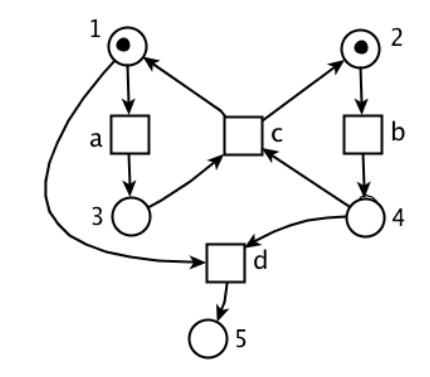
\includegraphics[scale = 0.4]{img/seq.jpg}
  \end{figure}
  si ha, per esempio, la seguente sequenza di occorrenza di eventi:
  \[\{1, 2\}[a > \{3, 2\}[b > \{3, 4\}[c > \{1, 2\}[b > \{1, 4\}[d > \{5\}\]
  arrivati in ``5'' abbiamo un caso finale, ovvero una situazione di
  \textbf{deadlock}, in quanto il sistema non può evolvere ulteriormente.\\
  Vediamo anche la seguente possibile sequenza di passi. In ``1'' e ``2'' sia
  ``a'' che ``b'' sono indipendenti e sono entrambi abilitati (scattano in
  maniera concorrente in un unico passo, ovviamente posso avere passi con lo
  scatto di un solo evento):
  \[\{1, 2\}[\{a, b\} > \{3, 4\}[\{c\} > \{1, 2\}[\{b\} > \{1, 4\}\]
  Come ricordato posso finire in una sequenza infinita.\\
  Potrei modellare un processo non sequenziale di $\Sigma$:
  \begin{figure}[H]
    \centering
    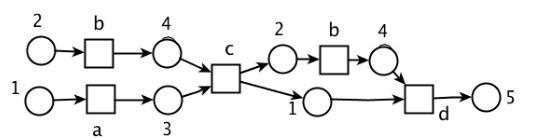
\includegraphics[scale = 0.4]{img/seq5.jpg}
  \end{figure}
\end{esempio}
Vediamo ora come modellare e registrare il comportamento del sistema. Un modo è
usando il \textbf{grafo dei casi raggiungibili} (equivalentemente a quanto si
faceva con il CCS).
\newpage
\begin{definizione}
  Il \textbf{grafo dei casi raggiungibili} di un sistema elementare
  $\Sigma=(B,E,F;c_{in})$ è il sistema di transizioni etichettato:
  \[CG_\Sigma=(C_\Sigma, U_\Sigma, A, c_{in})\]
  dove:
  \begin{itemize}
    \item $C_\Sigma$ è l'insieme dei nodi del grafo, ovvero gli stati globali,
    i casi raggiungibili dal sistema $\Sigma$    
    \item $U_\Sigma$, è l'alfabeto, ovvero i passi del sistema rappresentano
    l'alfabeto 
    \item $A$ è l'insieme di archi etichettati, formalmente definito come:
    \[A=\{(c,U,c')|\,c,c'\in C_\Sigma, U\in U_\Sigma, c[U>c'\}\]
    ovvero sono archi che connettono uno caso $c$ con un caso $c'$ e sono
    etichettati con un passo $U$ sse $U$ è abilitato in $c$ e porta in
    $c'$. Ovviamente $c$ e $c'$ sono devono essere raggiungibili e $U$ deve
    appartenere all'insieme dei passi di $\Sigma$
  \end{itemize}
  Esempio in figura \ref{fig:gra}.
\end{definizione}
\begin{figure}
  \centering
  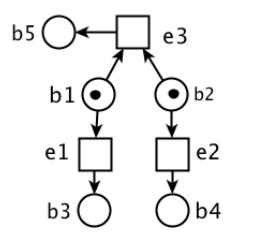
\includegraphics[scale = 0.5]{img/seq1.jpg}
  %\caption{Esempio di sistema $\Sigma$}
  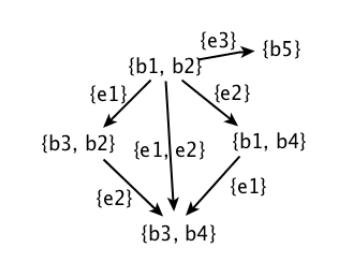
\includegraphics[scale = 0.5]{img/seq2.jpg}
  \caption{Esempio di sistema $\Sigma$ e il suo grafo dei casi del sistema
    $\Sigma$}
  \label{fig:gra}
\end{figure}
\subsection{Diamond Property}
Dato un sistema elementare $\Sigma = (B,E,F;c_{in})$ e il suo grafo dei casi
$CG_\Sigma=(C_\Sigma, U_\Sigma, A, c_{in})$ si ha 
che il grafo soddisfa una particolare proprietà, detta \textbf{diamond
  property}, tipica solo dei sistemi elementari.
\begin{definizione}
  La \textbf{diamond property} stabilisce una proprietà della struttura del
  grafo della rete elementare, ovvero, dati $U_1,U_2\in U_\Sigma$ tali che:
  \begin{itemize}
    \item $U_1\cap U_2=\emptyset$
    \item $U_1\neq\emptyset$
    \item $U_2\neq\emptyset$
  \end{itemize}
  e dati $c_i\in C_\Sigma$ allora vale, per esempio:
  \begin{figure}[H]
    \centering
    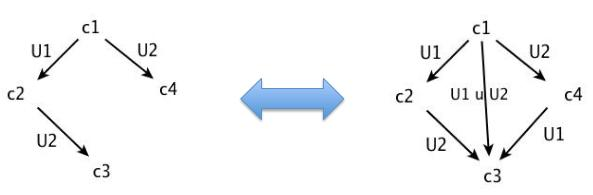
\includegraphics[scale = 0.6]{img/diam.jpg}
    \label{fig:dia}
  \end{figure}
  ovvero se posso rilevare come sottografo una struttura come quella a sinistra
  nell'immagine allora sicuramente tale sottografo contiene anche gli
  archi per ottenere l'immagine di destra. 
\end{definizione}
Si possono fare delle prove:
\begin{enumerate}
  \item \textbf{prima prova:}\\
  Dimostriamo che possiamo passare all'immagine di destra da quella di sinistra
  aggiungendo i due archi mancanti, nella figura \ref{fig:dia}.\\
  Per semplicità diciamo che $U_i$ è un singolo evento $e_i$, con $i=1,2$. Siano
  inoltre $c_1,c_2\in C_\Sigma$, ovvero sono casi raggiungibili, ed $e_1,e_2\in
  E$ tali che $c_1 [e_1 > c_2 [e_2 > \mbox{ e } c_1 [e_2 >$, i due eventi quindi
  sono abilitati in sequenza e da $c_1$ è anche abilitato $c_2$ . Si vuole
  dimostrare che: 
  \[(^\bullet e_1\cup e_1^\bullet)\cap(^\bullet e_2\cup e_2^\bullet)=\emptyset\]
  ovvero che i due eventi sono indipendenti, che sono entrambi abilitati e che
  sono eseguibili in qualsiasi ordine.
  \newpage
  Da $c_1 [e_1 > \mbox{ e }c_1 [e_2 >$ segue che:
  \begin{itemize}
    \item $^\bullet e_1\cap e_2^\bullet=\emptyset$
    \item $^\bullet e_2\cap e_1^\bullet=\emptyset$
  \end{itemize}
  infatti se $e_1$ e $e_2$ sono entrambi abilitati in $c_1$, le loro
  pre-condizioni sono vere e le post-condizioni false, e quindi non è possibile
  che una condizione sia contemporaneamente precondizione di $e_1$ (vera) e
  anche postcondizione di $e_2$ (falsa), e viceversa. Quindi le precondizioni
  di un evento sono disgiunte dalle postcondizioni dell'altro.\\
  Inoltre dal fatto che ho $c_1 [e_1 > c_2 [e_2$, ovvero che da $c_1$ è
  abilitato $e_1$ e che dopo lo scatto di $e_1$ è ancora abilitato $e_2$
  possiamo dire che:
  \begin{itemize}
    \item $e_1^\bullet\cap e_2^\bullet=\emptyset$
    \item $^\bullet e_1\cap\, ^\bullet e_2=\emptyset$
  \end{itemize}
  in $c_2$, infatti, le pre-condizioni di $e_1$ sono false mentre le
  precondizioni di $e_2$ sono vere e quindi $e_1$ e $e_2$ non possono avere
  precondizioni in comune; inoltre sempre in $c_2$ le postcondizioni di $e_1$
  sono vere, mentre quelle di $e_2$ sono false, e quindi $e_1$ e $e_2$ non
  possono avere post-condizioni in comune. Quindi le precondizioni dei due
  eventi sono disgiunte, come del resto anche le postcondizioni, in quanto i due
  eventi sono sequenziali.\\
  Si è quindi dimostrato che i due eventi hanno precondizioni e postcondizioni
  completamente disgiunte e quindi la tesi è verificata
  \item \textbf{seconda prova:}\\
  Analizzando la situazione:
  \begin{figure}[H]
    \centering
    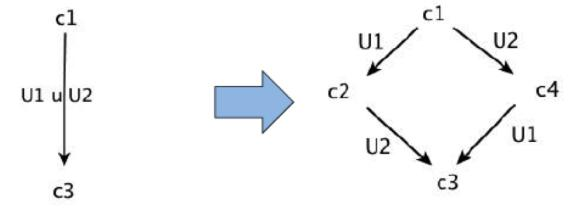
\includegraphics[scale = 0.45]{img/diam2.jpg}
  \end{figure}
  \newpage
  Si supponga che $U_1\cup U_2\in U_\Sigma$ e che si abbiano:
  \begin{itemize}
    \item $U_1\cap U_2=\emptyset$, ovvero sono disgiunti
    \item $U_1\neq\emptyset$
    \item $U_2\neq\emptyset$
  \end{itemize}
  allora se $c_1[(U_1\cup U_2)>c_3$, quindi è abilitato il passo $U_1\cup U_2$
  in $c_1$, sicuramente si ha che sono abilitati anche i singoli passi:
  \begin{itemize}
    \item $c_1[U_1>$
    \item $c_1[U_2>$
  \end{itemize}
  resta da dimostrare che dopo lo scatto di $U_1$ è ancora abilitato $U_2$ in
  $c_2$. Ma se $U_1\cup U_2$ è un passo abilitato significa che posso eseguirli
  in qualsiasi ordine, quindi anche prima $U_1$ e poi $U_2$, e questo comporta
  sicuramente che $U_2$ è abilitato e che porta a $c_3$. Analogamente invertendo
  $U_1$ e $U_2$, formalmente: 
  \begin{itemize}
    \item $c_1[U_1>c_2[U_2>c_3$
    \item $c_1[U_2>c_4[U_1>c_3$
  \end{itemize}
  Si dimostra così che l'immagine di sinistra comporta quella di destra.
\end{enumerate}
Grazie alla diamond property possiamo non considerare il grafo dei casi
raggiungibili ma solo il \textbf{grafo dei casi sequenziale}:
\begin{definizione}
  Un \textbf{grafo dei casi sequenziale} del sistema elementare
  $\Sigma=(B,E,F;c_{in})$ è una quadrupla:
  \[SCG_\Sigma=(C_\Sigma,E,A,c_{in})\]
  dove le etichette sono i singoli eventi (mentre il resto rimane definito come
  nel grafo dei casi raggiungibili). Formalmente si ha quindi che:
  \[A=\{(c,e,c')|\,c,c'\in C_\Sigma,\,e\in E:\, c[e>c'\}\]
  \begin{figure}[H]
    \centering
    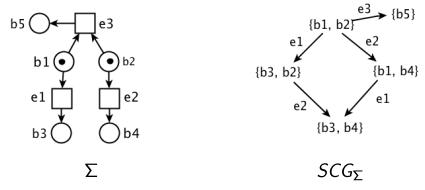
\includegraphics[scale = 0.6]{img/seq3.jpg}
    \caption{Esempio di grafo dei casi sequenziale}
  \end{figure}
  Si registra quindi l'occorrenza di un evento alla volta. Il grafo dei casi
  sequenziale è quindi il sistema di transizione con gli archi etichettati dai
  singoli eventi.
  \begin{figure}[H]
    \centering
    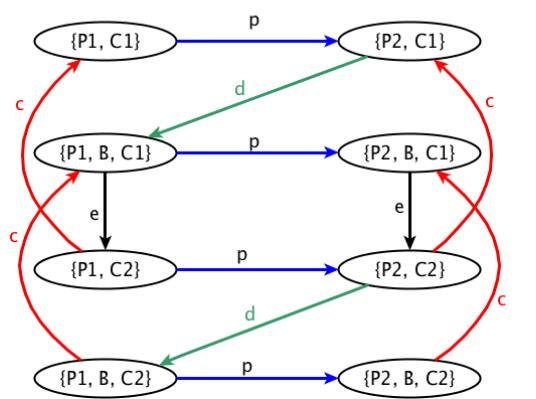
\includegraphics[scale = 0.4]{img/seqq.jpg}
    \caption{Esempio di grafo dei casi sequenziale dell'esempio con produttore
      e consumatore (con marche in $P1$ e $C1$)}
  \end{figure}
\end{definizione}
Riprendendo l'immagine precedente si ha che per la diamond property possono
aggiungere l'arco ``centrale'' che trasformerebbe nuovamente il grafo dei casi
sequenziale in quello dei casi raggiungibili quindi:
\textit{per la diamond property, nei sistemi elementari il grafo dei casi e il
  grafo dei casi sequenziale sono \textbf{sintatticamente equivalenti}, ovvero
  possono essere ricavati a vicenda.\\
  Questo implica il fatto che due sistemi elementari hanno grafi dei casi
  \textbf{isomorfi} sse hanno grafi dei casi sequenziali isomorfi.}
\subsection{Isomorfismo tra Sistemi di Transizione Etichettati}
Si ricorda che:
\begin{center}
  \textit{Si parla di isomorfismo quando due strutture complesse si possono
    applicare l'una sull'altra, cioè far corrispondere l'una all'altra, in modo
    tale che per ogni parte di una delle strutture ci sia una parte
    corrispondente nell'altra struttura; in questo contesto diciamo che due
    parti sono corrispondenti se hanno un ruolo simile nelle rispettive
    strutture.}
\end{center}
Diamo ora una definizione formale di isomorfismo tra sistemi di transizione
etichettati, che possono quindi essere grafi dei casi o grafi dei casi
sequenziali.
\begin{definizione}
  Siano dati due sistemi di transizione etichettati:\\
  $A_1 = (S_1,E_1,T_1,s_{01})$ e $A_2 = (S_2 , E_2 , T_2 , s_{02})$.\\
  e siano date due \textbf{mappe biunivoche}:
  \begin{enumerate}
    \item $\alpha:S_1\to S_2$, ovvero che passa dagli stati del primo sistema a
    quelli del secondo
    \item $\beta:E_1\to E_2$, ovvero che passa dagli eventi del primo sistema a
    quelli del secondo
  \end{enumerate}
  allora:
  \[\langle \alpha,\beta\rangle:A_1= (S_1 , E_1 , T_1 ,s_{01})\to A_2 = (S_2 ,
    E_2 , T_2 , s_{02})\]
  è un \textbf{isomorfismo} sse:
  \begin{itemize}
    \item $\alpha(s_{01})=s_{02}$, ovvero l'immagine dello stato iniziale del
    primo sistema coincide con lo stato iniziale del secondo
    \item $\forall s,s'\in S_1,\forall e\in E_1:\,(s,e,s')\in T_1
    \Leftrightarrow (\alpha(s),\beta(e),\alpha(s'))\in T_2$ ovvero per ogni
    coppia di stati del primo sistema, tra cui esiste un arco etichettato $e$,
    vale che esiste un arco, etichettato con l'immagine di $e$, nel secondo
    sistema che va dall'immagine del primo stato considerato del primo sistema
    all'immagine del secondo stato considerato del secondo sistema, e viceversa
  \end{itemize}
\end{definizione}
\begin{definizione}
  Si definiscono due \textbf{sistemi equivalenti} sse hanno grafi dei casi
  sequenziali, e quindi di conseguenza anche grafi dei casi, \emph{isomorfi}.\\
  Due sistemi equivalenti accettano ed eseguono le stesse sequenze di eventi
\end{definizione}
\subsection{Il Problema della Sintesi}
Si presenta ora un problema tipico dell'informatica, il \textbf{problema della
  sintesi}, ovvero dato un comportamento, o meglio una sua specifica, decidere
se esiste un'implementazione di tale specifica, ovvero un modello, che abbia
esattamente quel comportamento.\\
In questo caso dato un sistema di transizioni etichettato $A=(S,E,T,s_0)$, con:
\begin{itemize}
  \item $S$ insieme degli stati
  \item $E$ insieme delle etichette, ovvero degli eventi
  \item $T$ insieme delle transizioni
  \item $s_0$ stato iniziale
\end{itemize}
ci si propone di stabilire se esiste un sistema elementare
$\Sigma=(B,E,F;c_{in})$, tale che l'insieme degli eventi del sistema esattamente
l'insieme delle etichette di $A$ e tale che il suo grafo dei casi $SCG_\Sigma$
sia isomorfo ad $A$. Ci si propone anche di costruirlo.\\
Il problema è stato risolto mediante la cosiddetta \textbf{teoria delle regioni}
(che però non verrà trattato nel corso). Una \textbf{regione} comunque è un
  particolare sottoinsiemi di stati, legati tramite una certa condizione. Si può
  però dire che $A$ dovrà 
soddisfare la diamond property, in quanto altrimenti non sarebbe un sistema di
transizioni che potrebbe corrispondere al comportamento di un sistema
elementare.
\subsection{Contatti}
\begin{definizione}
  Sia $\Sigma = (B,E,F;c_{in})$ un sistema elementare e siano $e\in E$ un evento
  e $c\in C_\Sigma$ un caso raggiungibile dal caso iniziale. Allora si ha che
  $(e,c)$ è un \textbf{contatto} sse:
  \[^\bullet e\subseteq c \wedge e^\bullet \cap c \neq\emptyset\]
  Ovvero, in termini pratici, siamo nel caso in cui un evento $e$ ha le
  precondizioni vere, si ha quindi che $^\bullet e\subseteq c$, e l'evento non
  ha tutte le postcondizioni false, quindi $e^\bullet \cap c \neq\emptyset$,
  allora si dice che l'evento $e$ è in una situazione di contatto e quindi non
  può scattare
  \begin{figure}[H]
    \centering
    \begin{tikzpicture}[node distance=2cm,bend angle=45,auto]
      \node [place, tokens=1] (p0) [label=above:P2] {};
      \node [transition] (t1) [below right of = p0, label=left:d] {};
      \node [transition] (t2) [below left of = p0, label=left:p] {};
      \node [place] (p1) [below right of = t2, label=below:P1] {}; 
      \node [place, tokens=1] (p3) [right of = t1, label=above:B] {};
      \node [transition] (t4) [right of = p3, label=right:e] {};

      \node [place, tokens=1] (p2) [above right of = t4,label=above:C1] {}; 
      \node [transition] (t3) [below right of = p2, label=right:c] {};
      \node [place] (p4) [below right of = t4, label=below:C2]
      {}; 
      
      \path[-{Latex[width=2mm]}]
      (p0) edge (t1)
      (t1) edge (p1)
      (p1) edge (t2)
      (t2) edge (p0)
      (t1) edge (p3)
      (p3) edge (t4)
      (t4) edge (p4)
      (p4) edge (t3)
      (t3) edge (p2)
      (p2) edge (t4)
      ;
    \end{tikzpicture}
    \caption{Esempio dove l'evento $d$ è in una situazione di
      contatto}
  \end{figure}
\end{definizione}
\begin{definizione}
  Sia $\Sigma = (B,E,F;c_{in})$ un sistema elementare. Si dice che il sistema è
  \textbf{senza contatti} sse:
  \[\forall e\in E,\,\forall c\in C_\Sigma\mbox{ si ha che } ^\bullet
    e\subseteq c\Rightarrow e^\bullet\cap c=\emptyset\]
  ovvero per ogni evento e per ogni caso raggiungibile dal caso iniziale succede
  sempre che se le precondizioni sono vere, ovvero $^\bullet e\subseteq c$,
  allora le postcondizioni sono false, ovvero disgiunte dal caso considerato
  ($e^\bullet\cap c=\emptyset$)
\end{definizione}
Ci si chiede se sia possibile trasformare un sistema elementare $\Sigma$, con
contatti, in uno $\Sigma'$, senza contatti, senza però modificarne il
comportamento.\\
La risposta a questo quesito è affermativa e la procedura consiste
nell'aggiungere a $\Sigma$ il complemento di ogni condizione che crea situazione
di contatto, ottenendo così un sistema $\Sigma'$ con grafo dei casi isomorfo a
quello di $\Sigma$.\\ 
Per aggiungere il complemento, data la condizione $x$, si aggiunge la condizione
$not\,\, x$ che sarà vera tutte le volte che $x$ è falsa e viceversa. Per
ottenere questo risultato la nuova condizione avrà come pre-eventi i
post-eventi di $x$ e come post-eventi i pre-eventi di $x$. Ovvero
connetto la nuova condizione agli stessi eventi di quella vecchia ma con archi
orientati in senso opposto. Ovviamente le inizializzazioni delle due condizioni
dovranno essere opposte (una vera e l'altra falsa).
\begin{figure}[H]
  \centering
  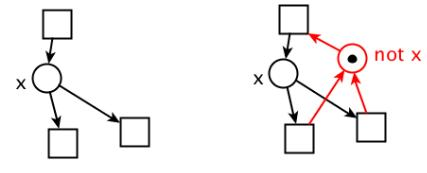
\includegraphics[scale = 0.6]{img/con2.jpg}
  \caption{Esempio con l'ottenimento del complemento di un sistema}
\end{figure}
Se un sistema è senza contatti si ha una regola di contatto semplificata:
\begin{definizione}
  Sia $\Sigma = (B,E,F;c_{in})$ un sistema elementare \textbf{senza
    contatti}. Sapendo che se le precondizioni di un evento sono vere allora
  sicuramente le postcondizioni di quell'evento sono false in quel caso. Dato
  che questo avviene per ogni evento e per ogni caso raggiungibile dal caso
  iniziale per verificare che un evento $e$ sia abilitato in un caso
  raggiungibile $c$ è sufficiente verificare che le precondizioni di $e$ siano
  vere (in quanto automaticamente le postcondizioni saranno false). In
  maniera formale quindi si ha che: 
  \[c[e\mbox{ sse } ^\bullet e\subseteq c,\,\,\mbox{ con } e\in E,c\in
    C_\Sigma\]
  semplificando di molto la \textbf{regola di scatto}:
\end{definizione}
\begin{figure}[H]
  \centering
  \begin{tikzpicture}[node distance=2cm,bend angle=45,auto]
      \node [place, tokens=1] (p0) [label=above:P2] {};
      \node [transition] (t1) [below right of = p0, label=left:d] {};
      \node [transition] (t2) [below left of = p0, label=left:p] {};
      \node [place] (p1) [below right of = t2, label=below:P1] {}; 
      \node [place, tokens=1] (p31) [above right  of = t1, label=above:B1] {};
      \node [place] (p32) [ below right of = t1, label=below:B2] {};
      \node [transition] (t4) [below right of = p31, label=right:e] {};

      \node [place, tokens=1] (p2) [above right of = t4,label=above:C1] {}; 
      \node [transition] (t3) [below right of = p2, label=right:c] {};
      \node [place] (p4) [below right of = t4, label=below:C2]
      {}; 
      
      \path[-{Latex[width=2mm]}]
      (p0) edge (t1)
      (t1) edge (p1)
      (p1) edge (t2)
      (t2) edge (p0)
      (t1) edge (p32)
      (p32) edge (t4)
      (t4) edge (p31)
      (p31) edge (t1)
      
      (t4) edge (p4)
      (p4) edge (t3)
      (t3) edge (p2)
      (p2) edge (t4)
      ;
    \end{tikzpicture}
  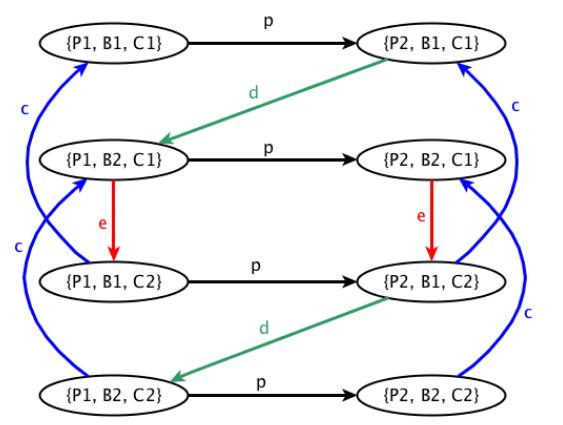
\includegraphics[scale = 0.4]{img/con33.jpg}
  \caption{Esempio con il complemento del sistema produttore-consumatore (dove è
    stato aggiunto solo il complemento di ``buffer-pieno'', ottenendo così sia
    $B1$ che $B2$, in quanto le altre condizioni avevano già il loro
    complemento). In aggiunta si ha anche il grafo dei casi sequenziale
    corrispondente al nuovo sistema senza contatti (grafo che è isomorfo a
    quello ottenibile al sistema con contatti)}
  \label{fig:con}
\end{figure}
\subsection{Situazioni Fondamentali}
\subsubsection{Sequenza}
\begin{definizione}
  Sia $\Sigma = (B,E,F;c_{in})$ un sistema elementare, con contatti o meno
  e siano $c\in C_\Sigma$ un caso raggiungibile dal caso iniziale e $e_1,e_2\in
  E$ due eventi.\\
  Si ha che $e_1$ ed $e_2$ sono \textbf{in sequenza} nel caso
  raggiungibile $c$ sse:
  \[c[e_1>\wedge\, \neg c[e_2\wedge c[e_1e_2>\]
  ovvero in $c$ è abilitato $e_1$ ma non $e_2$ ma, dopo lo scatto di $e_1$,
  $e_2$ diventa abilitato. Quindi in $c$ è possibile attivare prima $e_1$ e poi
  $e_2$ in sequenza.\\
  Si ha quindi una relazione di \textbf{dipendenza causale tra $e_1$ ed $e_2$},
  ovvero qualche postcondizione di $e_1$ è precondizione di $e_2$ (che quindi
  può occorrere solo se precedentemente è occorso $e_1$).
  \begin{figure}[H]
    \centering
    \begin{tikzpicture}[node distance=2cm,bend angle=45,auto]
      \node [place, tokens=1] (p0)  {};
      \node [transition] (t1) [right of = p0, label=above:$e_1$] {};
      \node [place] (p1) [above right  of = t1] {};
      \node [place] (p2) [right of = t1] {};
      \node [transition] (t2) [right  of = p1, label=above:$e_2$] {};
      \node [place] (p3) [right  of = t2] {};
      {}; 
      
      \path[-{Latex[width=2mm]}]
      (p0) edge (t1)
      (t1) edge (p1)
      (t1) edge (p2)
      (p1) edge (t2)
      (t2) edge (p3)
      ;
    \end{tikzpicture}
    \caption{Esempio di sequenza tra $e_1$ ed $e_2$}
  \end{figure}
\end{definizione}
\subsubsection{Concorrenza}
\begin{definizione}
  Sia $\Sigma = (B,E,F;c_{in})$ un sistema elementare, con contatti o meno
  e siano $c\in C_\Sigma$ un caso raggiungibile dal caso iniziale e $e_1,e_2\in
  E$ due eventi. \\
  Si ha che i due eventi sono \textbf{concorrenti} nel caso
  raggiungibile $c$ sse:
  \[c[\{e_1,e_2\}>\]
  ovvero se possono essere abilitati in unico passo o, detto in maniera
  diversa, se sono indipendenti ed entrambi abilitati in $c$
  \begin{figure}[H]
    \centering
    \begin{tikzpicture}[node distance=2cm,bend angle=45,auto]
      \node [place, tokens=1] (p0)  {};
      \node [place, tokens=1] (p00) [below of = p0] {};
      \node [transition] (t1) [right of = p0, label=above:$e_1$] {};
      \node [transition] (t2) [right of = p00, label=above:$e_2$] {};
      \node [place] (p1) [right  of = t1] {};
      \node [place] (p2) [right of = t2] {};
      \node [transition] (t3) [right of = p1] {};
      \node [place] (p3) [right of = t3] {};
      {}; 
      
      \path[-{Latex[width=2mm]}]
      (p0) edge (t1)
      (t1) edge (p1)
      (p1) edge (t3)
      (p00) edge (t2)
      (t2) edge (p2)
      (p2) edge (t3)
      (t3) edge (p3)
      ;
    \end{tikzpicture}
    \caption{Esempio di concorrenza tra $e_1$ ed $e_2$}
  \end{figure}
\end{definizione}
\subsubsection{Conflitto}
\begin{definizione}
  Sia $\Sigma = (B,E,F;c_{in})$ un sistema elementare, con contatti o meno
  e siano $c\in C_\Sigma$ un caso raggiungibile dal caso iniziale e $e_1,e_2\in
  E$ due eventi.\\
  Si ha che $e_1$ ed $e_2$ sono in conflitto sse:
  \[c[e_1>\,\wedge\, c[e_2 \wedge\,\neg c[\{e_1,e_2\}>\]
  ovvero i due eventi sono entrambi abilitati (quindi le precondizioni sono vere
  mentre le postcondizioni son false) ma l'occorrenza di uno disabilità
  l'altro, quindi non possono essere abilitati in un unico passo, in quanto non
  sono indipendenti. Ci sono due casi:
  \begin{enumerate}
    \item i due eventi hanno una precondizione in comune, e in tal caso si parla
    di \textbf{conflitto forward} (ovvero \textit{in avanti})
    \begin{figure}[H]
      \centering
      \begin{tikzpicture}[node distance=2cm,bend angle=45,auto]
        \node [place, tokens = 1] (p0)  {};
        \node [transitionv] (t1) [above right of = p0, label=above:$e_1$] {};
        \node [transitionv] (t2) [below right of = p0, label=below:$e_2$] {};
        \node [place] (p1) [right  of = t1] {};
        \node [place] (p2) [right of = t2] {};
        {}; 
        
        \path[-{Latex[width=2mm]}]
        (p0) edge (t1)
        (t1) edge (p1)
        (p0) edge (t2)
        (t2) edge (p2)

        ;
      \end{tikzpicture}
      \caption{Esempio di conflitto forward tra $e_1$ ed $e_2$}
    \end{figure}
    \item i due eventi hanno una postcondizione in comune, e in tal caso si parla
    di \textbf{conflitto backward} (ovvero \textit{all'indietro})
    \begin{figure}[H]
      \centering
      \begin{tikzpicture}[node distance=2cm,bend angle=45,auto]
        \node [place, tokens = 1] (p0)  {};
        \node [place, tokens = 1] (p00) [below of = p0] {};
        \node [transitionv] (t1) [right of = p0, label=above:$e_1$] {};
        \node [transitionv] (t2) [right of = p00, label=below:$e_2$] {};
        \node [place] (p1) [right  of = t1] {};
        {}; 
        
        \path[-{Latex[width=2mm]}]
        (p0) edge (t1)
        (t1) edge (p1)
        (p00) edge (t2)
        (t2) edge (p1)
        ;
      \end{tikzpicture}
      \caption{Esempio di conflitto backward tra $e_1$ ed $e_2$}
    \end{figure}
  \end{enumerate}
  Si ha quindi una situazione di \textbf{non determinismo}, non essendo
  specificato quale dei due eventi scatterà prima (e lo scatto di uno impedisce
  lo scatto dell'altro).
  Posso ritrovarmi nel caso in cui effettivamente un evento scatta, cambiando lo
  stato del sistema. In tal caso, in un'ottica completamente deterministica, si
  deve assumere che \textbf{l'ambiente} abbia fornito un'informazione
  riguardo il conflitto, ovvero c'è stato qualcosa di esterno che ha permesso ad
  uno dei due eventi di scattare ugualmente. Ho quindi guadagnato
  dell'informazione. 
  \begin{figure}[H]
    \centering
    \begin{tikzpicture}[node distance=2cm,bend angle=45,auto]
      \node [place] (p0)  {};
      \node [transitionv] (t1) [above right of = p0, label=above:$e_1$] {};
      \node [transitionv] (t2) [below right of = p0, label=below:$e_2$] {};
      \node [place, tokens=1] (p1) [right  of = t1] {};
      \node [place] (p2) [right of = t2] {};
      {}; 
      
      \path[-{Latex[width=2mm]}]
      (p0) edge (t1)
      (t1) edge (p1)
      (p0) edge (t2)
      (t2) edge (p2)

      ;
    \end{tikzpicture}
    \caption{Esempio di conflitto con l'intervento dell'ambiente tra $e_1$ ed
      $e_2$ (con conseguente guadagno di informazione)} 
  \end{figure}
  Ci sono però casi in cui in ogni caso non si può avere informazione su quale
  esempio sia scattato. Si può ipotizzare che tale informazione fosse presente
  nello stato precedente del sistema (una sola condizione attiva, per
  esempio). Quindi l'informazione, finita nell'ambiente (ricevuta
  dall'ambiente), si è persa.
  \begin{figure}[H]
    \centering
    \begin{tikzpicture}[node distance=2cm,bend angle=45,auto]
        \node [place] (p0)  {};
        \node [place] (p00) [below of = p0] {};
        \node [transitionv] (t1) [right of = p0, label=above:$e_1$] {};
        \node [transitionv] (t2) [right of = p00, label=below:$e_2$] {};
        \node [place, tokens = 1] (p1) [right  of = t1] {};
        {}; 
        
        \path[-{Latex[width=2mm]}]
        (p0) edge (t1)
        (t1) edge (p1)
        (p00) edge (t2)
        (t2) edge (p1)
        ;
      \end{tikzpicture}
    \caption{Esempio di conflitto tra $e_1$ ed
      $e_2$ con conseguente perdita di informazione (si può ipotizzare, per
      esempio, che nello stato precedente la precondizione di $e_1$ fosse attiva
      mentre quella dio $e_2$ fosse inattiva)} 
  \end{figure}
  Il modello, nell'ottica di Petri, non è quindi un \textbf{modello chiuso} ma è
  in grado di comunicare con l'ambiente (in sintonia con le teorie della
  fisica). 
\end{definizione}
\subsubsection{Confusione}
\begin{definizione}
  La situazione di \textbf{confusione} è una \textit{mistura} di situazioni di
  concorrenza e di conflitto. Si hanno 2 tipi di confusione, entrambe
  ammissibili: 
  \begin{enumerate}
    \item detta \textbf{confusione asimmetrica} considera il fatto di avere un
    caso raggiungibile e due eventi abilitati, nella figura $e_1$ ed $e_2$, in
    maniera concorrente in $c$, che nella figura consiste nel caso
    $\{b_1,b_2,b_3\}$. I due eventi sono quindi indipendenti. Nella figura lo
    scatto dei due eventi porterebbe allo stato $c'=\{b_4,b_5\}$. Bisogna
    analizzare però nel dettaglio il sistema. Se prima occorre $e_1$ non si ha
    alcun conflitto mentre se occorre prima $e_2$ (che porterebbe in
    $\{b_1,b_3,b_4\}$) si crea un conflitto tra $e_1$ ed $e_3$, che viene
    risolto a favore di $e_1$ e a sfavore di $e_3$. \textbf{Non è possibile
      stabilire oggettivamente se è stato sciolto un conflitto}. Sono quindi in
    una situazione di confusione in quanto non so se è stata effettuata o meno
    una scelta.
    \begin{figure}[H]
      \centering
      \begin{tikzpicture}[node distance=2cm,bend angle=45,auto]
        %\node [place, tokens = 1] (p0)  {};
        \node [transition] (t1) [ label=right:$e_2$] {};
        \node [place, tokens = 1] (p0) [left of = t1,  label=left:$b_2$] {};
        \node [place] (p1) [below  of = t1,  label=left:$b_4$] {};
        \node [place, tokens = 1] (p2) [left  of = p1, label=left:$b_3$] {};
        \node [place, tokens = 1] (p3) [left  of = p2,  label=left:$b_1$] {};
        \node [transition] (t2) [below of = p1, label=left:$e_1$] {};
        \node [transition] (t3) [below of = p3, label=right:$e_3$] {};
        \node [place] (p4) [below of = t2, label=left:$b_5$] {};;
        \node [place] (p5) [below of = t3,  label=left:$b_6$] {};
        {}; 
        
        \path[-{Latex[width=2mm]}]
        (p0) edge (t1)
        (t1) edge (p1)
        (p1) edge (t2)
        (p2) edge (t2)
        (p2) edge (t3)
        (p3) edge (t3)
        (t2) edge (p4)
        (t3) edge (p5)
        ;
      \end{tikzpicture}
      \caption{Esempio di confusione asimmetrica tra $e_1$ ed $e_2$} 
    \end{figure}
    Una soluzione che vedremo sarà la scomposizione in più componenti del
    sistema 
    \item detta \textbf{confusione simmetrica}, nome dovuto al fatto che la rete
    risulta disegnata in modo simmetrico, comportando delle
    problematiche. Prendiamo nell'immagine il caso raggiungibile $c=\{b_1,b_2\}$
    e i due eventi $e_1$ ed $e_3$, abilitati in maniera concorrente. Si ha che
    $c[\{e_1,e_3\}>c'$, con $c'=\{b_3,b_5\}$. Anche in questo caso si hanno dei
    conflitti, infatti sia $e_1$ che $e_3$ sono in conflitto con $e_2$ (in
    quanto se uno dei due viene eseguito $e_2$ non può più occorrere). Anche in
    questo caso non posso stabilire se il conflitto è stato risolto nel momento
    in cui arrivo in $c'$ (ovvero se si è deciso di fare $e_1$ piuttosto che
    $e_2$ o $e_3$ piuttosto che $e_2$).\\
    Anche in questo caso potremo dividere in componenti (una che esegue $e_1$ ed
    $e_2$ e un'altra che esegue $e_1$ ed $e_3$, con $e_2$ che è una
    sincronizzazione tra le due componenti).\\
    Non si può dire chi ha deciso e chi ha la responsabilità di decidere quale
    evento deve occorrere, se alla componente di $b_1$ o a quella di $b_2$.\\
    \begin{figure}[H]
      \centering
      \begin{tikzpicture}[node distance=2cm,bend angle=45,auto]
        \node [place, tokens = 1] (p0) [label=left:$b_1$] {};
        %\node [place, tokens = 1] (p1) [right of = p0, label=left:$b_2$] {};
        \node [transition] (t1) [below left of = p0, label=right:$e_1$] {};
        \node [transition] (t2) [below right of = p0, label=right:$e_2$] {};
        \node [place, tokens = 1] (p1) [above right of=t2,label=left:$b_2$] {};
        \node [transition] (t3) [below right of = p1, label=right:$e_3$] {};
        \node [place] (p3) [below of = t1, label=left:$b_3$] {};;
        \node [place] (p4) [below of = t2,  label=left:$b_4$] {};
        \node [place] (p5) [below of = t3,  label=left:$b_5$] {};
        {}; 
        
        \path[-{Latex[width=2mm]}]
        (p0) edge (t1)
        (p0) edge (t2)
        (p1) edge (t2)
        (p1) edge (t3)
        (t1) edge (p3)
        (t2) edge (p4)
        (t3) edge (p5)
        ;
      \end{tikzpicture}
      \caption{Esempio di confusione simmetrica tra $e_1$ ed $e_2$} 
    \end{figure}
  \end{enumerate}
  Petri era convinto, nella sua visione deterministica e senza conflitti, che
  l'avere una situazione di confusione nel modello fosse dovuto al non aver
  esplicitato alcuni aspetti o di aver costruito male il modello, con
  informazioni parziali e non complete sul modello e sull'ambiente.\\
  Un altro studioso, Einar Smith, molto vicino a Petri ha invece dimostrato come
  la confusione sia inevitabile
\end{definizione}
Vediamo un esempio famoso, detto della \textbf{mutua esclusione}, portato da
Smith per spiegare come la confusione sia inevitabile nella realtà.
\newpage
\begin{esempio}
  Si analizza il seguente sistema:
  \begin{figure}[H]
    \centering
    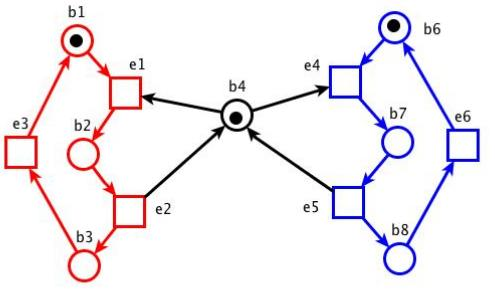
\includegraphics[scale = 0.4]{img/mes.jpg} 
  \end{figure}
  In rosso e in Blu abbiamo specificate le due componenti del sistema, che
  condividono una risorsa, ovvero la condizione $b_4$, che rappresenta che la
  risorsa è libera e a disposizione. L'evento $e_1$ e evento $e_4$ rappresentano
  eventi di acquisizione della risorsa (rispettivamente per la prima e per la
  seconda componente) e quindi le loro precondizioni rappresentano la necessità
  di acquisirla. Tra questi due eventi c'è una \textbf{situazione di
    conflitto}. Le condizioni $b_2$ e $b_7$, ovvero le rispettive postcondizioni
  dei due eventi, rappresentano che la risorsa è in uso per la rispettiva
  componente mentre gli eventi $e_2$ ed $e_5$ rappresentano il rilascio della
  risorsa condivisa, sempre per la rispettiva componente, arrivando
  rispettivamente nella componente $b_3$ e $b_8$. Ovviamente la risorsa
  non può essere contemporaneamente in uso da entrambe le risorse, quindi $b_2$
  e $b_7$ non possono essere contemporaneamente marcate, ovvero vere, e per
  questo si parla di \textit{mutua esclusione} (se una delle due è vera l'altra
  deve essere necessariamente falsa). D'altro canto gli
  eventi $e_3$ ed $e_6$ possono invece occorrere in modo concorrente senza
  conflitti.\\
  Scrivendo formalmente si ha che, nel caso che la risorsa sia stata acquisita
  dalla componente rossa e successivamente rilasciata:
  \[\{b_3,b_4,b_6\}[\{e_3,e_4\}>\{b_1,b_7\}\]
  ma se scatta prima $e_3$ ho il conflitto tra $e_1$ ed $e_4$, se scatta prima
  $e_4$ non ho conflitti con $e_1$. Quindi non ho informazioni sulla risoluzione
  del conflitto.\\
  \textbf{Capire se è confusione simmetrica}
\end{esempio}
\subsection{Sottoreti}
Partiamo subito con una definizione formale:
\begin{definizione}
  Siano $N=(B,E,F)$ e $N_1=(B_1,E_1,F_1)$ due reti elementari.\\
  Si dice che $N_1$ è \textbf{sottorete} di $N$ sse:
  \begin{itemize}
    \item $B_1\subseteq B$, quindi l'insieme delle condizioni della rete $N_1$
    è sottoinsieme di quello della rete $N$
    \item $E_1\subseteq E$, quindi l'insieme degli eventi della rete $N_1$
    è sottoinsieme di quello della rete $N$
    \item $F_1=F\cap[(B_1\times E_1)\cup (E_1\times B_1)]$, ovvero la relazione
    di flusso di $N_1$ è definita come la restrizione della relazione di flusso
    di $N$ rispetto alle condizioni e $B_1$ e agli eventi $E_1$ (tengo quindi
    solo gli archi di $N$ che connettono eventi e condizioni di $N_1$)
  \end{itemize}
\end{definizione}
\begin{definizione}
  Siano $N=(B,E,F)$ e $N_1=(B_1,E_1,F_1)$ due reti elementari.\\
  Si dice che $N_1$ è \textbf{sottorete generata da} $B_1$ di $N$ (ovvero di
  sottorete generata da un insieme di condizioni) sse:
  \begin{itemize}
    \item $B_1\subseteq B$, quindi l'insieme delle condizioni della rete $N_1$
    è sottoinsieme di quello della rete $N$
    \item $E_1=\, ^\bullet B_1\cup B_1^\bullet$, ovvero come eventi si
    hanno tutti quegli eventi che sono collegati in $N$ alle condizioni incluse
    nell'insieme di condizioni $B_1$, prendendo quindi tutti i pre-eventi e i
    post-eventi delle condizioni dell'insieme $B_1$
    \item $F_1=F\cap[(B_1\times E_1)\cup (E_1\times B_1)]$, ovvero la relazione
    di flusso di $N_1$ è definita come la restrizione della relazione di flusso
    di $N$ rispetto alle condizioni $B_1$ e agli eventi $E_1$
  \end{itemize}
  Non ho quindi una sottorete generata da un insieme arbitrario di condizioni ed
  eventi ma questi ultimi sono direttamente presi in relazione all'insieme delle
  condizioni scelto
\end{definizione}
\begin{definizione}
  Siano $N=(B,E,F)$ e $N_1=(B_1,E_1,F_1)$ due reti elementari.\\
  Si dice che $N_1$ è \textbf{sottorete generata da} $E_1$ di $N$ (ovvero di
  sottorete generata da un insieme di eventi) sse:
  \begin{itemize}
    \item $B_1=\,^\bullet E_1\cup E_1^\bullet$, ovvero come condizioni si
    hanno tutte quelle condizioni che sono collegati in $N$ agli eventi inclusi
    nell'insieme di eventi $E_1$, prendendo quindi tutte e precondizioni e le
    postcondizioni degli eventi dell'insieme $E_1$
    \item $E_1\subseteq E$, quindi l'insieme degli eventi della rete $N_1$
    è sottoinsieme di quello della rete $N$
    \item $F_1=F\cap[(B_1\times E_1)\cup (E_1\times B_1)]$, ovvero la relazione
    di flusso di $N_1$ è definita come la restrizione della relazione di flusso
    di $N$ rispetto alle condizioni $B_1$ e agli eventi $E_1$
  \end{itemize}
  Non ho quindi una sottorete generata da un insieme arbitrario di condizioni ed
  eventi ma le prime sono direttamente prese in relazione all'insieme degli
  eventi scelto
\end{definizione}
\begin{esempio}
  Tornando all'esempio della mutua esclusione:
  \begin{figure}[H]
    \centering
    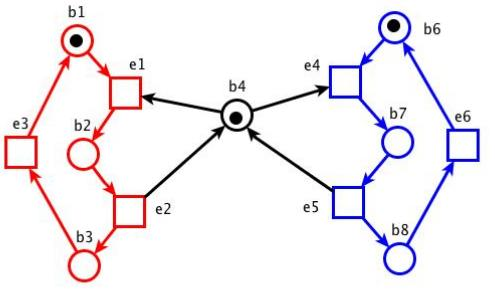
\includegraphics[scale = 0.4]{img/mes.jpg} 
  \end{figure}
  si ha, per esempio:
  \begin{itemize}
    \item in rosso si ha la sottorete $N'=(\{b_1,b_2,b_3\},
    \{e_1,e_2,e_3\},F')$, che è la sottorete generata  dall'insieme di
    condizioni $B'=\{b_1,b_2,b_3\}$ 
    \item in blu si ha la sottorete $N'=(\{b_6,b_7,b_8\},
    \{e_4,e_5,e_6\},F')$, che è la sottorete generata dall'insieme di condizioni
    $B'=\{b_6,b_7,b_8\}$
    \item si ha la sottorete $N'=(\{b_2,b_4,b_7\},\{e_1,e_2,e_4,e_5\},F')$, che
    è la sottorete generata  dall'insieme di condizioni $B'=\{b_2,b_4,b_7\}$
    \item si ha la sottorete $N'=(\{b_1,b_2,b_3,b_4\},\{e_1,e_2,e_3\},F')$, che
    è la sottorete generata da  dall'insieme di eventi $E'=\{e_1,e_2,e_3\}$
  \end{itemize}
\end{esempio}
\subsection{Operazioni di Composizione per Reti di Petri}
Data una rete $N=(B,E,F,c_0)$ questa può essere ottenuta componendo altre reti
di Petri. Si hanno in letteratura 3 modi principali:
\begin{enumerate}
  \item la \textbf{composizione sincrona}
  \item la \textbf{composizione asincrona}
  \item la \textbf{composizione mista, tra sincrona e asincrona}
\end{enumerate}
\newpage
Iniziamo informalmente a vedere degli esempi pratici.
\begin{esempio}
  Supponiamo di avere i modelli di due componenti, $N_1$, con un evento che
  corrisponde ad un'azione di invio, ed $N_2$, con un evento che corrisponde ad
  un'azione di ricezione:
  \begin{figure}[H]
    \centering
    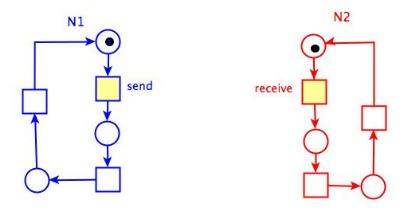
\includegraphics[scale = 0.5]{img/sinc.jpg} 
  \end{figure}
  Supponiamo che invio e ricezione siano eventi corrispondenti all'handshacking,
  ovvero l'invio avviene solo se può avvenire la ricezione.\\
  Vado quindi a sincronizzare questi due eventi, che diventano quindi un'unico
  evento nella rete composta, che è abilitato se le due precondizioni, nelle due
  componenti sono entrambe vere: 
  \begin{figure}[H]
    \centering
    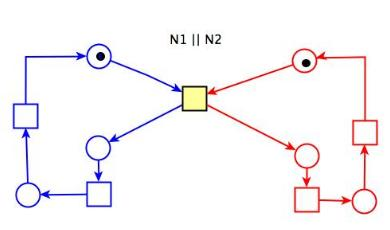
\includegraphics[scale = 0.5]{img/sinc2.jpg} 
  \end{figure}
  La composizione viene indicata con:
  \[N_1||N_2\]
  Lo scatto dell'evento, in maniera sincrona, rende vere le postcondizioni nelle
  due componenti e false le due precondizioni.\\
  Abbiamo appena visto un esempio di \textbf{composizione sincrona}
\end{esempio}
\begin{esempio}
  Supponiamo di avere i modelli di due componenti, $N_1$, che invia in un canale
  un messaggio (per esempio in un buffer), e $N_2$, che riceverà il messaggio
  solo quando esso sarà disponibile:
  \begin{figure}[H]
    \centering
    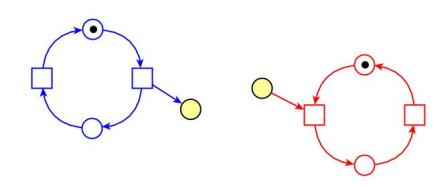
\includegraphics[scale = 0.5]{img/asinc.jpg} 
  \end{figure}
  In questo caso, a differenza dell'esempio precedente, non identifichiamo
  eventi ma condizioni. Identifico quindi il canale (le due condizioni) come uno
  solo, che avrà il pre-evento in una componente e il post-evento nell'altra.\\
  Quindi il pre-evento, nella componente $N_1$, può scattare solo se questa
  nuova condizione condivisa, il canale, è libera, indipendentemente dalla
  componente $N_2$. D'altro canto l'evento in $N_2$ può scattare solo se la
  condizione condivisa è marcata, indipendentemente dallo stato della prima
  componente, liberando il canale di comunicazione.\
  Avvio e ricezione (dopo che il messaggio è stato inviato può essere letto in
  un qualsiasi futuro) non sono sincronizzati e si ha quindi a che fare con
  un esempio di \textbf{composizione asincrona}.\\
  Si avrebbe:
  \begin{figure}[H]
    \centering
    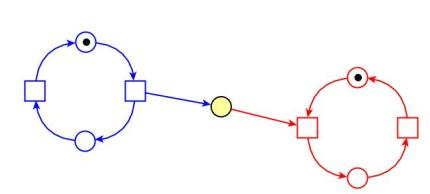
\includegraphics[scale = 0.5]{img/asinc2.jpg} 
  \end{figure}
\end{esempio}
Sarà interessante studiare come la composizione di due componenti, per esempio,
senza deadlock non comporta, in generale, l'ottenimento di una rete priva di
deadlock.
\section{Processi non sequenziali}
Parliamo ora di sistemi non sequenziali, ad ordini parziali.\\
Vediamo un esempio sempre usato da Petri.
Petri pensò ad un sistema in cui diversi omini, spostandosi avanti nel tempo,
portassero dei secchi per andare a spegnere un fuoco (dato che il sentiero  è
stretto si studia protocollo per cui se hanno il secchio vuoto si muovono a
sinistra fino alla fonte d'acqua e a quel punto ci si sposta a destra). Se due
omini si incontrano lungo la strada si scambiano 
il secchio e invertono la direzione di marcia:
\begin{figure}[H]
  \centering
  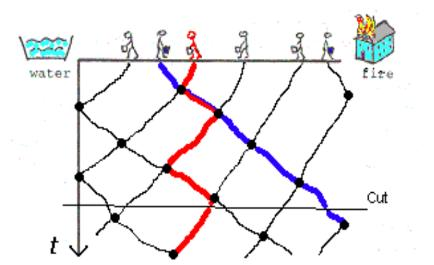
\includegraphics[scale = 0.5]{img/fire.jpg} 
\end{figure}
Un modello classico è quello di far scorrere il tempo come nell'immagine vedendo
gli spostamenti di ogni omino. Nell'immagine si identifica in rosso la storia di
un omino e in blu la storia del secchio pieno.
Ma a Petri non va bene questo modello avendo a che fare col il 
tempo, avendo un modello non discreto.\\
Cerca quindi un modello combinatorio in cui si hanno varie
configurazioni che possono essere osservate (con quindi non necessariamente una
sola scala del tempo).
Si può osservare una configurazione del tipo:
\begin{figure}[H]
  \centering
  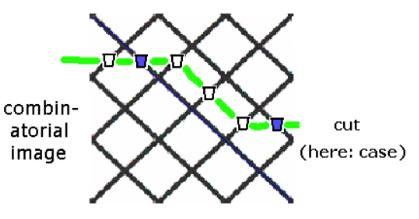
\includegraphics[scale = 0.5]{img/fire2.jpg} 
\end{figure}
con relazioni di dipendenza degli eventi (le righe blu) e situazioni di
indipendenza (la riga verde).\ 
Gli omini potrebbero essere quindi
modellati da una rete con gli incontri tra omini che diventano
sincronizzazioni. L'evoluzione del sistema può essere registrato salvando
informazioni vere. Nel sistema la prima transizione a sinistra è quindi il
prelevamento dell'acqua e l'ultimo a destra il versamento sul fuoco:
\begin{figure}[H]
  \centering
  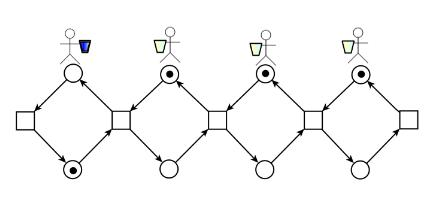
\includegraphics[scale = 0.5]{img/inc.jpg} 
\end{figure}
Gli eventi in mezzo sono i cambiamenti di secchio.\\
l'ordine degli archi segue il secchio, verso sinistra con il secchio vuoto e
verso destra con il secchio pieno. Le condizioni in alto praticamente sono il
secchio vuoto mentre in basso pieno.\\
L'evoluzione del sistema posso memorizzarlo tramite condizioni vere. 
Possiamo quindi produrre la rete in base alle condizioni che possono scattare
(in corrispondenza degli elementi della rete),
ottenendo:
\begin{figure}[H]
  \centering
  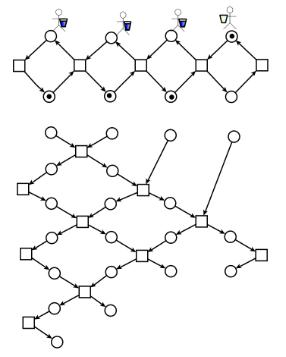
\includegraphics[scale = 0.7]{img/inc2.jpg} 
\end{figure}
Tale modello è infinito.\\
\newpage
Posso modellare i vari percorsi tramite linee colorate (percorso del secchio
pieno in blu, percorso dell'omino in rosso, secchio vuoto in giallo,
etc$\ldots$) con quelle tratteggiate 
in alto (verde) che rappresentano lo stato iniziale e quelle in basso (viola)
quello finale, dove blocco il sistema
(dopo il quale si ricomincia da capo):
\begin{figure}[H]
  \centering
  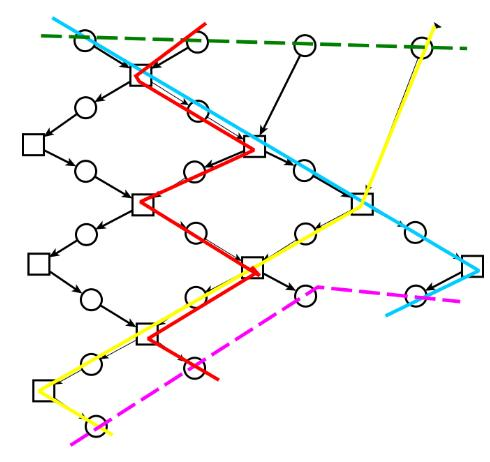
\includegraphics[scale = 0.5]{img/inc3.jpg} 
\end{figure}
Tra le varie linee colorate (non quelle tratteggiate) si hanno relazioni di
dipendenza. \\
Definiamo il tutto in modo formale.
\begin{definizione}
  Definiamo:
  \[N=(B,E,F)\]
  come una \textbf{rete causale}, detta anche rete di occorrenze senza conflitti,
  sse:
  \begin{itemize}
    \item $\forall b\in B:|\,^{\bullet}b|\leq 1\land |b^{\bullet}|\leq 1$, ovvero
    non si hanno conflitti, quindi per ogni condizione si ha al più un pre
    evento e un post evento (avendo quindi al più un arco entrante e al più uno
    uscente)
    
    \item $\forall a,y\in B\cup E:(x,y)\in F^+\implies (y,x)\not\in F^+$, ovvero
    non si hanno cicli, quindi presi due elementi collegati da una sequenza di
    archi orientati, avendo un cammino tra i due elementi ($F^+$ è la chiusura
    transitiva della relazione $F$) non ho anche un cammino opposto tra i due
    \item $\forall e\in E:\{x\in B\cup E|\,xF^*e\}$ è finito, ovvero si ha un
    numero finito di pre-elementi di un certo elemento
  \end{itemize}
  Sono quindi reti che registrano un comportamento e quindi non si hanno
  conflitti (che in caso sono sciolti registrando solo quello che è
  effettivamente successo e non quello che potrebbe succedere). Si registra una
  run del sistema. Non si hanno nemmeno cicli perché ogni ripetizione
  dell'evento viene concatenata a quella prima (come detto nell'esempio dopo le
  righe tratteggiate in viola si cominciava da capo).\\
  La rete può essere quindi si infinita ma è composta da un insieme di elementi
  finito che si ripete. In ogni caso il passato di un evento è finito e
  registrato, anche se nel complesso il comportamento è infinito ``in
  avanti''. \\
  Con una rete causale si possono non distinguere più condizioni ed eventi.

\end{definizione}
Ad una rete causale è possibile associare un ordine parziale:
\[(X,\leq)=(B\cup E, F^*)\]
Dicendo che un elemento ``è minore'' di un altro se esiste un cammino orientato
dall'uno all'altro (si specifica che $F^*$ non mi farà mai identificare $x$ con
$x$).
\begin{esempio}
  Vediamo un esempio di rete causale:
   \begin{figure}[H]
    \centering
    \begin{tikzpicture}[node distance=2cm,bend angle=45,auto]
      \node [place] (p0)  {};
      \node [transitionv] (t1) [right of = p0] {};
      \node [place] (p1) [above right of = t1] {};;
      \node [place] (p2) [below right of = t1] {};
      \node [transitionv] (t2) [right of = p1] {};
      \node [place] (p3) [right of = t2] {}; 
      
      \path[-{Latex[width=2mm]}]
      (p0) edge (t1)
      (t1) edge (p1)
      (t1) edge (p2)
      (p1) edge (t2)
      (t2) edge (p3)
      ;
    \end{tikzpicture}
  \end{figure}
  che quindi avendo un ordine parziale ed essendo causale posso scrivere come:
  \begin{figure}[H]
    \centering
    \begin{tikzpicture}[node distance=2cm,bend angle=45,auto]
      \node [place] (p0)  {};
      \node [place] (t1) [right of = p0] {};
      \node [place] (p1) [above right of = t1] {};;
      \node [place] (p2) [below right of = t1, label=below:$a$] {};
      \node [place] (t2) [right of = p1, label=above:$b$] {};
      \node [place] (p3) [right of = t2] {}; 
      
      \path[-{Latex[width=2mm]}]
      (p0) edge (t1)
      (t1) edge (p1)
      (t1) edge (p2)
      (p1) edge (t2)
      (t2) edge (p3)
      ;
    \end{tikzpicture}
  \end{figure}
  L'ordine \textbf{parziale} si rileva dal fatto che, per esempio, non si ha
  alcuna relazione d'ordine tra $a$ e $b$.
\end{esempio}
\begin{esempio}
  Vediamo anche due esempi di reti non causali:
  \begin{figure}[H]
    \centering
    \begin{tikzpicture}[node distance=2cm,bend angle=45,auto]
      \node [place] (p0)  {};
      \node [transition] (t1) [right of = p0] {};
      \node [place] (p1) [below of = t1] {};
      \node [transition] (t2) [below of = p1] {};
      \node [place] (p2) [left of = t2] {};
      \node [transition] (t3) [above of = p2] {};
      %\node [place] (p3) [right of = t3] {}; 
      
      \path[-{Latex[width=2mm]}]
      (p0) edge (t1)
      (t1) edge (p1)
      (p1) edge (t2)
      (t2) edge (p2)
      (p2) edge (t3)
      (t3) edge (p0)
      ;
    \end{tikzpicture}
  \end{figure}
  avendo un ciclo.\\
  Oppure:
  \begin{figure}[H]
    \centering
    \begin{tikzpicture}[node distance=2cm,bend angle=45,auto]
      \node [place] (p0)  {};
      \node [transitionv] (t1) [above right of = p0] {};
      \node [transitionv] (t2) [below right of = p0] {};
      \node [place] (p2) [right of = t1] {};
      \node [place] (p3) [right of = t2] {};
      \path[-{Latex[width=2mm]}]
      (p0) edge (t1)
      (p0) edge (t2)
      (t1) edge (p2)
      (t2) edge (p3)
      ;
    \end{tikzpicture}
  \end{figure}
  Avendo un conflitto.
\end{esempio}
\begin{definizione}
  Data una rete causale $N=(B,E,F)$ e dato un ordine parziale $(X, \leq)$ con
  $X=B\cup E$ si ha che si può interpretare la relazione d'ordine come
  indipendenza o dipendenza causale, ovvero presi $x,y\in X$ come elementi che
  occorrono nella storia di $X=B\cup E$ si hanno le seguenti diciture:
  \begin{itemize}
    \item $x\leq y$ (avendo un cammino da $x$ a $y$) corrisponde a \textbf{$x$
      causa $y$}, ovvero si ha una relazione di dipendenza causale tra i due
    \item $x \mbox{ \textbf{li} }y$ indica che $x\leq y\lor y\leq x$ e quindi
    corrisponde a \textbf{$x$ e $y$ sono casualmente dipendenti}. Si ha che
    \textbf{li} può venire letto come \textit{linea} ($x$ in linea con $y$) 
    avendo che uno dei due precede l'altro
    \item $x \mbox{ \textbf{co} }y$ indica che $\neg(x< y)\land \neg(y < x)$ e
    quindi corrisponde a \textbf{$x$ e $y$ sono casualmente indipendenti},
    avendo che i due elementi non si precedono a vicenda, non avendo ordine tra
    loro. Si ha che \textbf{co} sta per \textit{concurrency}
  \end{itemize}
\end{definizione}
\begin{esempio}
  Presa la rete causale (già compattata):
  \begin{figure}[H]
    \centering
    \begin{tikzpicture}[node distance=2cm,bend angle=45,auto]
      \node [place] (p0) [label=left:$a$] {};
      \node [place] (p1) [above right of = p0, label=above:$b$] {};;
      \node [place] (p2) [right of = p0,  label=above:$c$] {};
      \node [place] (p3) [right of = p1,  label=right:$d$] {}; 
      
      \path[-{Latex[width=2mm]}]
      (p0) edge (p1)
      (p0) edge (p2)
      (p1) edge (p3)
      ;
    \end{tikzpicture}
  \end{figure}
  Si ha che:
  \begin{itemize}
    \item $b \mbox{ \textbf{co} }c$
    \item $c \mbox{ \textbf{co} }d$
    \item $\neg (b \mbox{ \textbf{co} }d)$
    \item $c \mbox{ \textbf{li} }a$
    \item $a \mbox{ \textbf{li} }d$
    \item $\neg (c \mbox{ \textbf{li} }d)$
  \end{itemize}
\end{esempio}
Si ha quindi che \textbf{\textit{li} \textnormal{e} co} sono:
\begin{itemize}
  \item simmetriche
  \item \textbf{non} transitive
  \item riflessive
\end{itemize}
che sono comunque proprietà derivate dalla teoria degli ordini parziali.\\
Possiamo ora considerare sottoinsiemi dell'ordine parziali in cui la relazione
\textbf{li} e la relazione \textbf{co} sono transitive.
\begin{definizione}
  Data una rete causale $N=(B,E,F)$ e dato un ordine parziale $(X, \leq)$ con
  $X=B\cup E$ definiamo:
  \[C\subseteq X\]
  come:
  \begin{itemize}
    \item \textbf{co-set} sse $\forall x,y\in C:\, x\mbox{ \textbf{co }}y$,
    quindi $C$ è una clique della relazione \textbf{co}
    \item \textbf{taglio} sse $C$ è un co-set massimale (tutti gli elementi nel
    taglio sono in relazione \textbf{co})
  \end{itemize}
  Definiamo $C$ come co-set massimale sse $\forall\,y\in X\backslash C$ si ha
  che:
  \[\exists c\in C:\,y\,\,\,\cancel{\mathbf{co}}\,\,\,c\]
  (nel dettaglio esiste almeno un $c$). \\
  Quindi in $C$ definito o come \textbf{co-set} o come \textbf{taglio} si ha che
  vale la transitività.\\
  
  Definiamo:
  \[L\subseteq X\]
  come:
  \begin{itemize}
    \item \textbf{li-set} sse $\forall x,y\in L:\, x\mbox{ \textbf{li }}y$
    \item \textbf{linea} sse $L$ è un li-set massimale
  \end{itemize}
  \textit{rivedere la seguente affermazione}:\\
  Definiamo $L$ come li-set massimale sse $\forall\,y\in X\backslash L$ si ha
  che:
  \[\exists l\in L:\,y\,\,\,\cancel{\mathbf{li}}\,\,\,l\]
  Si ha quindi che:
  \begin{itemize}
    \item in un \textbf{co-set} la relazione \textbf{co} è transitiva
    \item in un \textbf{li-set} la relazione \textbf{li} è transitiva.
  \end{itemize}
  Tagli e linee possono essere fatti sia di condizioni che di eventi.
\end{definizione}
\begin{esempio}
  Tornando all'esempio del secchio:
  \begin{figure}[H]
    \centering
    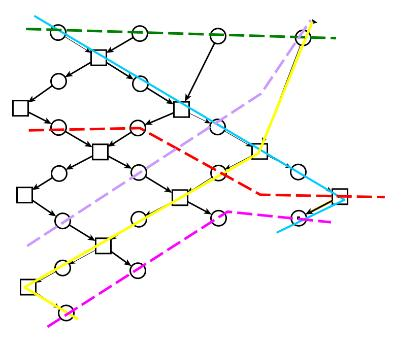
\includegraphics[scale = 0.5]{img/ta.jpg} 
  \end{figure}
  si ha che:
  \begin{itemize}
    \item la storia del secchio è un insieme di elementi in relazione
    \textbf{li} e, nello specifico, ad esempio la parte azzurra o quella gialla,
    è una \textit{linea} che descrive un sottoprocesso
    \item le parti tratteggiate, sono invece
    un co-set e, nel dettaglio, sono un 
    taglio (infatti se cerco di aggiungere un qualsiasi altro elemento otterrei
    una relazione di dipendenza con uno degli elementi già presenti)
  \end{itemize}
\end{esempio}
\textbf{I tagli fatti di sole condizioni rappresentano casi raggiungibili
  (nell'immagine quello verde che quello viola che quello viola-chiaro)}.\\
Una rete causale quindi registra il comportamento di un sistema elementare.\\
Si hanno quindi, con i tagli, possibili osservazioni di configurazioni possibili
nella storia del sistema.
\begin{definizione}
  Grazie alle reti causali, preso un elemento $x\in X$, possiamo definire:
  \begin{itemize}
    \item $past(x)$, ovvero il passato dell'elemento, tutti gli elementi in
    relazione $\leq$ di $x$
    \item $future(x)$, ovvero il futuro dell'elemento, tutti gli elementi in
    relazione $\geq$ di $x$
  \end{itemize}
  Visualizzabili, per esempio, nell'immagine, rispettivamente in rosso e blu:
  \begin{figure}[H]
    \centering
    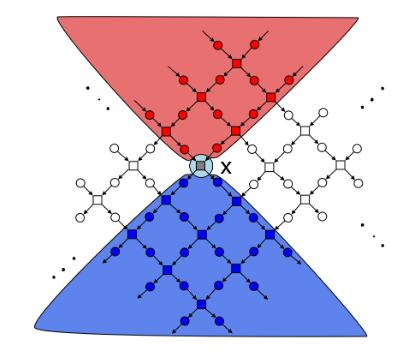
\includegraphics[scale = 0.5]{img/pf.jpg} 
  \end{figure}
  Gli elementi nell'anti-cono (la parte bianca) sono in relazione \textbf{co}
  con $x$ e quindi possono essere concorrenti.
\end{definizione}
\begin{definizione}
  Data una rete causale $N=(B,E,F)$ e dato un ordine parziale $(X, \leq)$ con
  $X=B\cup E$ definiamo che la rete è \textbf{K-densa} se ogni linea ed ogni
  taglio si intersecano in un punto, tutti hanno un punto comune. Formalmente:
  \[\forall\,h\in Linee(N),\forall\,c\in Tagli(N):|h\cap c|=1\]
  Con $Linee(N)$ e $Tagli(N)$ che sono rispettivamente li insiemi di tutte le
  linee e dei tagli.\\
  Se $N$ è finita è anche \textbf{K-densa}, se sono infinite non è detto.\\
  Una rete non K-densa potrebbe essere (in rosso una linea e in blu un taglio):
  \begin{figure}[H]
    \centering
    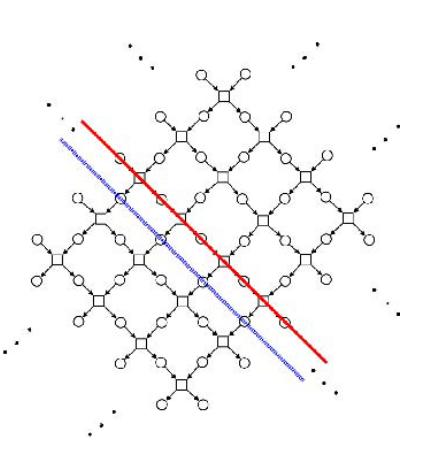
\includegraphics[scale = 0.36]{img/de1.jpg} 
  \end{figure}
  (si nota che è una rete infinita).\\
  e una K-densa:
  \begin{figure}[H]
    \centering
    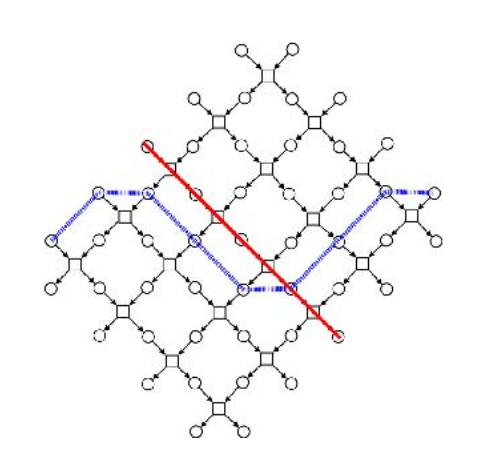
\includegraphics[scale = 0.36]{img/de2.jpg} 
  \end{figure}
  (si nota che è una rete finita).\\
  ($K$ significa combinatoria).
\end{definizione}
\begin{esempio}
  Vediamo anche il solito esempio della mutua esclusione:
  \begin{figure}[H]
    \centering
    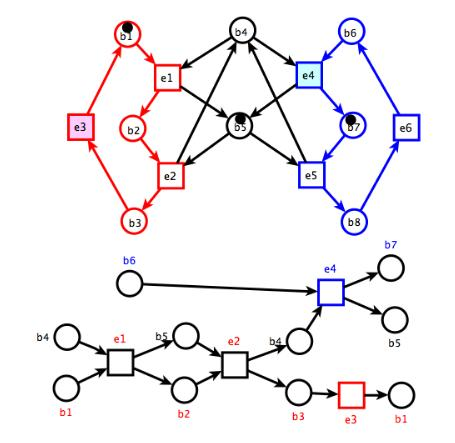
\includegraphics[scale = 0.5]{img/de3.jpg} 
  \end{figure}
  Con sia il sistema elementare che la rete causale associata (dove si vede ad
  esempio che $e_4$ ed $e_3$ sono in relazione \textbf{co}, le prime tre
  condizioni a sinistra ($b_1,b_4,b_6$) sono un taglio anche le
  ultime a destra ($b_1,b_5,b_7$)). 
\end{esempio}
\begin{definizione}
  Sia $\Sigma=(S,T,F,c_{in})$ un sistema elementare senza contatti e finito,
  tale che $S\cup T$ sia finito. Si ha che, con $\phi$ che mappa dalla rete
  causale al sistema elementare: 
  \[\langle N=(B,E,F), \phi\rangle\]
  è un processo non sequenziale di $\Sigma$ sse:
  \begin{itemize}
    \item $(B,E,F)$ è una rete causale (si ammettono condizioni isolate)
    \item $\phi:B\cup E\to S\cup T$ è una mappa tale che:
    \begin{itemize}
      \item $\phi(B)\subseteq S, \phi(E)\subseteq T$
      \item $\forall x,y\in B\cup E:\phi(x)=\phi(y)\implies (x\leq y)\lor (y\leq
      x)$ non avendo quindi concorrenza
      \item $\forall e\in E:\phi(\,^\bullet e)=\,^\bullet
      \phi(e)\land\phi(e^\bullet)=\phi(e)^\bullet$ quindi le precondizioni di un
      evento nella rete causale devono corrispondere alle pre dell'evento nel
      sistema elementare (e così anche per le post)
      \item $\phi(Min(N))=c_{in}$,\\ con $Min(N)=\{x\in B\cup E|\nexists
      y_(y,x)\in F\}$ che sono gli stati locali iniziali, ovvero se prendo gli
      elementi minimali della rete 
      causali, che non hanno un arco entrante, essi sono mappati nel caso
      iniziale del sistema elementare
    \end{itemize}
  \end{itemize}
  Se ho queste proprietà la rete causale è una registrazione del sistema
  elementare.\\
  In tal caso si ha che $N=(B,E,F)$ è K-densa (sia che sia finita che infinita),
  avendo il sistema di partenza finito. Le linee sono quindi sottoprocessi
  sequenziali e i tagli possibili configurazioni sempre raggiungibili.\\
  Inoltre si ha che:
  \[\forall K\in B\mbox{ K è B-taglio di } N \mbox{ t.c. } K \mbox{ è finito}
    \land \exists c\in C_\Sigma:\phi(K)=c\]
\end{definizione}
Dato un sistema ho tanti processi non sequenziali che rappresentano esecuzioni
del sistema. Ci si chiede quindi se ho un unico oggetto che rappresenta tutti i
possibili run del sistema.
\begin{figure}[H]
  \centering
  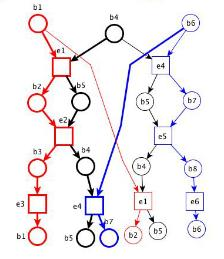
\includegraphics[scale = 0.6]{img/be4.jpg}
  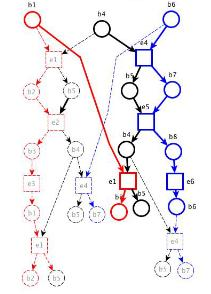
\includegraphics[scale = 0.6]{img/be5.jpg} 
  \caption{Esempio con più processi del modello della mutua esclusione
    modellati da un’unica rete con conflitti in avanti.}
\end{figure}
\textbf{Su slide, quelle dedicate agli esercizi, ulteriori esempi.}
\begin{definizione}
  Data una rete causale $N=(B,E,F)$, con $X=B\cup E$, diciamo che è una
  \textbf{rete di occorrenze} sse:
  \begin{itemize}
    \item $\forall\,b\in B:|\,^\bullet b|=1$, ovvero ho conflitti solo in
    avanti
    \item $\forall\,x,y\in B\cup E:(x,y)\in F^+\implies (y,x)\not\in F^+$,
    ovvero non ho cicli, in quanto le ripetizioni sono già registrate
    \item $\forall\,e\in E:\{x\in B\cup E|xF^*e\}$, ovvero il passato di un
    evento, è finito 
    \item la \textbf{relazione di conflitto} $\#$ non è riflessiva, avendo:
    \[\#\subset X\times X\]
    definita come:
    \[x\# y\iff \exists e_1,e_2\in E:\,^\bullet e_1\cap \,^\bullet e_2\neq
      \emptyset \land e_1\leq x\land e_2\leq y\]
    ovvero due elementi sono in conflitto sse sono in ``alternativa'' ovvero se
    si hanno due eventi che condividono precondizioni (sicuramente non le post
    non avendo conflitti in avanti) con i due eventi che causano i due elementi
    $x$ e $y$, allora anche questi due sono in conflitto. Vediamo degli esempi:
    \begin{figure}[H]
      \centering
      \begin{tikzpicture}[node distance=1.7cm,bend angle=45,auto]
        \node [place] (p0)  {};
        \node [transitionv] (t1) [above right of = p0] {};
        \node [transitionv] (t2) [below right of = p0] {};
        \node [place] (p2) [right of = t1] {};
        \node [place] (p3) [above right of = t2] {};
        \node [place] (p4) [right of = t2, label=below:$x$] {};
        \node [transitionv] (t3) [right of = p2, label=above:$y$] {};
        \node [place] (p5) [right of = t3] {};
        % \node [place] (p3) [right of = t3] {}; 
        
        \path[-{Latex[width=2mm]}]
        (p0) edge (t1)
        (p0) edge (t2)
        (t1) edge (p2)
        (p2) edge (t3)
        (t3) edge (p5)
        (t2) edge (p3)
        (t2) edge (p4)
        ;
      \end{tikzpicture}
      \caption{Esempio con $x$ e $y$ non in conflitto. Nel dettaglio questa è
        una rete di occorrenze}
      \label{fig:esemp}
    \end{figure}
    \begin{figure}[H]
      \centering
      \begin{tikzpicture}[node distance=1.7cm,bend angle=45,auto]
        \node [place] (p0) [label=left:$p$] {};
        \node [transitionv] (t1) [above right of = p0, label=above:$e_1$] {};
        \node [transitionv] (t2) [below right of = p0, label=below:$e_2$] {};
        \node [place] (p2) [right of = t1] {};
        \node [place] (p3) [above right of = t2] {};
        \node [place] (p4) [right of = t2] {};
        \node [transitionv] (t3) [right of = p2, label=above:$z$] {};
        \node [place] (p5) [right of = t3] {};
        % \node [place] (p3) [right of = t3] {}; 
        
        \path[-{Latex[width=2mm]}]
        (p0) edge (t1)
        (p0) edge (t2)
        (t1) edge (p2)
        (p2) edge (t3)
        (t3) edge (p5)
        (p3) edge (t3)
        (t2) edge (p3)
        (t2) edge (p4)
        ;
      \end{tikzpicture}
      \caption{Esempio con $z$ che è in conflitto con se stessa (avendo $e_1<z$
        e $e_2<z$, con i due eventi che condividono $p$) e quindi non può
        essere una rete di occorrenze}
    \end{figure}
  \end{itemize}
  È comunque possibile associare ad una rete di occorrenze $N$ un ordine
  parziale. 
\end{definizione}

\begin{definizione}
  Sia $\Sigma=(S,T,F,c_{in})$ un sistema elementare senza contatti e
  finito. Si ha che:
  \[\langle N=(B,E,F), \phi\rangle\]
  è un \textbf{processo ramificato} di $\Sigma$ sse:
  \begin{itemize}
    \item $(B,E,F)$ è una rete di occorrenze (si ammettono condizioni isolate,
    volendo poter registrare il caso iniziale come un insieme di condizioni che
    magari non vengono modificate)
    \item $\phi:B\cup E\to S\cup T$ è una mappa tale che:
    \begin{itemize}
      \item $\phi(B)\subseteq S, \phi(E)\subseteq T$
      \item $\forall e_1,e_2\in E:(\,^\bullet e_1=\,^\bullet e_2\land
      \phi(e_1)=\phi(e_2))\implies e_1=e_2$, ovvero se due eventi condividono le
      precondizioni e corrispondono allo stesso eventi del sistema secondo la
      mappa allora necessariamente sono lo stesso evento
      \item $\forall e\in E:\phi(\,^\bullet e)=\,^\bullet
      \phi(e)\land\phi(e^\bullet)=\phi(e)^\bullet$ quindi le precondizioni di un
      evento nella rete causale devono corrispondere alle pre dell'evento nel
      sistema elementare (e così anche per le post)
      \item $\phi(Min(N))=c_{in}$, quindi il taglio iniziale deve essere il caso
      iniziale del sistema
    \end{itemize}
  \end{itemize}
\end{definizione}
\begin{esempio}
  Riprendendo il solito esempio di mutua esclusione:
  \begin{figure}[H]
    \centering
    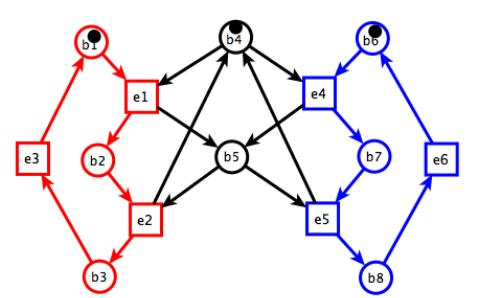
\includegraphics[scale = 0.45]{img/ram0.jpg} 
  \end{figure}
  \newpage
  si ha il seguente processo ramificato:
  \begin{figure}[H]
    \centering
    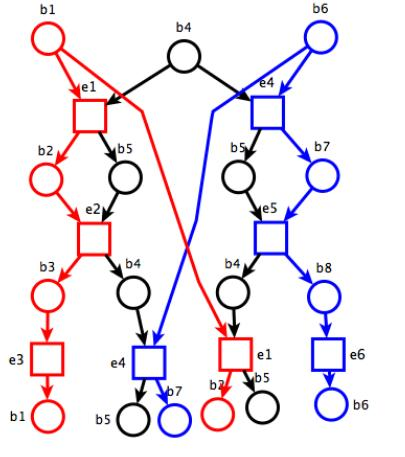
\includegraphics[scale = 0.45]{img/ram.jpg} 
  \end{figure}
  
\end{esempio}
\noindent
Cerchiamo ora di definire meglio l'unfolding, quell'oggetto che rappresenta
tutti i possibili sottoprocessi non sequenziali di del sistema, ovvero tutti i
possibili comportamenti del sistema.\\
Definiamo prima dei ``prerequisiti''.
\begin{definizione}
  Sia $\Sigma=(S,T,F,c_{in})$ un sistema elementare senza contatti e finito, e
  siano:
  \[\Pi_1=\langle N_1;\phi_1\rangle\]
  \[\Pi_2=\langle N_2;\phi_2\rangle\]
  due processi ramificati di $\Sigma$.\\
  Si ha che $\Pi_1$ è un \textbf{prefisso} di $\Pi_2$ (e quindi $\Pi_1$ è un
  sottoprocesso di $\Pi_2$) sse:
  \begin{itemize}
    \item $N_1$ è una sottorete di $N_2$
    \item $\phi_{2|N_1}=\phi_1$ ovvero $\phi_2$ ristretto a $N_1$  è uguale a
    $\phi_1$ 
  \end{itemize}
  Si ha che $\Sigma$ ammette un unico processo ramificato che è massimale
  rispetto alla relazione di prefisso tra processi e tale processo è detto
  \textbf{unfolding} di $\Sigma$:
  \[Unf(\Sigma)\]
  Quindi è il processo ramificato più grande, largo il più possibile e lungo
  infinito se il sistema ha comportamento ciclico.\\
  Ha senso studiare un prefisso finito dell'unfolding che permette di
  determinare tutto l'unfolding.\\
  Tale processo non sequenziale è un processo ramificato:
  \[\Pi=\langle N;\phi\rangle\]
  tale che $N$ è una rete causale, senza conflitti. Il processo $\Pi$ è anche
  detto \textbf{run} di $N$.\\
  L'unfolding tiene traccia di tutti i processi sequenziali di un sistema
  elementare. 
\end{definizione}
\textbf{Rivedere bene questa parte (lezione 30 novembre, con anche parte di
  esercizi)}.\\

\begin{esempio}
  Riprendendo il solito esempio di mutua esclusione si ha il seguente unfolding
  infinito:
  \begin{figure}[H]
    \centering
    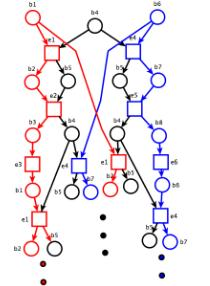
\includegraphics[scale = 0.45]{img/unf.jpg} 
  \end{figure}
\end{esempio}
Si è cercato di capire se un prefisso dell'unfolding basti a studiare l'intero
sistema.
\begin{definizione}
  Definiamo \textbf{prefisso completo} un prefisso che include tutti i casi
  raggiungibili.
\end{definizione}
Più si ha concorrenza e più la discrepanza tra unfolding e sistema di
transizioni aumenta a favore del prefisso finito dell'unfolding (???). Con
concorrenza alta si hanno algoritmi più efficienti di calcolo dell'unfolding (e
anche di model checking).
% \subsection{Reti posti e transizioni}
% Vediamo ora una nuova classe delle \textit{reti di Petri}, detta \textbf{reti
% Posti e Transizioni}, permette di rappresentare un sistema in modo più
% compatto, sono una sorta di \textit{ripiegamento} dei sistemi
% elementari. Partiamo quindi da un esempio:
% \begin{esempio}
%   prendiamo in studio sempre il sistema produttore-consumatore:
%   Sia nella versione con contatto:
%   \begin{figure}[H]
%     \centering
%     \begin{tikzpicture}[node distance=2cm,bend angle=45,auto]
%       \node [place, tokens=1] (p0) [label=above:P2] {};
%       \node [transition] (t1) [below right of = p0, label=left:d] {};
%       \node [transition] (t2) [below left of = p0, label=left:p] {};
%       \node [place] (p1) [below right of = t2, label=below:P1] {}; 
%       \node [place, tokens=1] (p3) [right of = t1, label=above:B] {};
%       \node [transition] (t4) [right of = p3, label=right:e] {};

%       \node [place, tokens=1] (p2) [above right of = t4,label=above:C1] {}; 
%       \node [transition] (t3) [below right of = p2, label=right:c] {};
%       \node [place] (p4) [below right of = t4, label=below:C2]
%       {}; 

%       \path[-{Latex[width=2mm]}]
%       (p0) edge (t1)
%       (t1) edge (p1)
%       (p1) edge (t2)
%       (t2) edge (p0)
%       (t1) edge (p3)
%       (p3) edge (t4)
%       (t4) edge (p4)
%       (p4) edge (t3)
%       (t3) edge (p2)
%       (p2) edge (t4)
%       ;
%     \end{tikzpicture}
%   \end{figure}
%   che senza:
%   \begin{figure}[H]
%     \centering
%     \begin{tikzpicture}[node distance=2cm,bend angle=45,auto]
%       \node [place, tokens=1] (p0) [label=above:P2] {};
%       \node [transition] (t1) [below right of = p0, label=left:d] {};
%       \node [transition] (t2) [below left of = p0, label=left:p] {};
%       \node [place] (p1) [below right of = t2, label=below:P1] {}; 
%       \node [place, tokens=1] (p31) [above right  of = t1, label=above:B1] {};
%       \node [place] (p32) [ below right of = t1, label=below:B2] {};
%       \node [transition] (t4) [below right of = p31, label=right:e] {};

%       \node [place, tokens=1] (p2) [above right of = t4,label=above:C1] {}; 
%       \node [transition] (t3) [below right of = p2, label=right:c] {};
%       \node [place] (p4) [below right of = t4, label=below:C2]
%       {}; 

%       \path[-{Latex[width=2mm]}]
%       (p0) edge (t1)
%       (t1) edge (p1)
%       (p1) edge (t2)
%       (t2) edge (p0)
%       (t1) edge (p32)
%       (p32) edge (t4)
%       (t4) edge (p31)
%       (p31) edge (t1)

%       (t4) edge (p4)
%       (p4) edge (t3)
%       (t3) edge (p2)
%       (p2) edge (t4)
%       ;
%     \end{tikzpicture}
%   \end{figure}
%   Suppongo di voler modellare il sistema in modo che il buffer possa avere un
%   numero determinato di posizioni, per esempio 2 (il buffer può quindi
%   depositare fino a due elementi). Si ottiene quindi:
%   \begin{figure}[H]
%     \centering
%     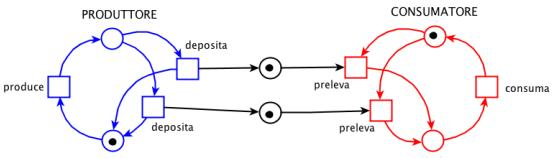
\includegraphics[scale = 0.6]{img/pt3.jpg} 
%   \end{figure}
%   Dove si hanno due posizioni del buffer (e quindi basta che una sia vuota per
%   permettere al produttore di depositare) a disposizione del sistema. Si nota
%   come l'aumento dei buffer complica drasticamente la modellazione del sistema.
%   Si cerca quindi una soluzione più compatta, compattando gli eventi
%   \textit{deposita} e \textit{preleva} e dando nuova notazione al buffer. Si
%   ottiene:
%   \begin{figure}[H]
%     \centering
%     \begin{tikzpicture}[node distance=2cm,bend angle=45,auto]
%       \node [place] (p0) [label=above:P2] {};
%       \node [transition] (t1) [below right of = p0, label=left:d] {};
%       \node [transition] (t2) [below left of = p0, label=left:p] {};
%       \node [place, tokens = 1] (p1) [below right of = t2, label=below:P1] {}; 
%       \node [place, tokens=2] (p3) [right of = t1, label=above:$\mbox{B,
%         capacità=2}$] {}; 
%       \node [transition] (t4) [right of = p3, label=right:e] {};

%       \node [place, tokens=1] (p2) [above right of = t4,label=above:C1] {}; 
%       \node [transition] (t3) [below right of = p2, label=right:c] {};
%       \node [place] (p4) [below right of = t4, label=below:C2]
%       {}; 
      
%       \path[-{Latex[width=2mm]}]
%       (p0) edge (t1)
%       (t1) edge (p1)
%       (p1) edge (t2)
%       (t2) edge (p0)
%       (t1) edge (p3)
%       (p3) edge (t4)
%       (t4) edge (p4)
%       (p4) edge (t3)
%       (t3) edge (p2)
%       (p2) edge (t4)
%       ;
%     \end{tikzpicture}
%   \end{figure}
%   con il buffer che diventa anche un \textbf{contatore} del numero di elementi
%   presenti al suo interno. Un buffer a due posizioni diventa quindi una
%   condizione non più booleana, detta \textbf{Posto}, con una \textbf{capacità}
%   pari a 2. Il produttore non può produrre oltre la capacità.\\
%   Con questa rappresentazione non ho più alcuna difficoltà nel rappresentare più
%   posizioni del buffer in quanto basta aumentare la capacità. Ho però perso
%   delle informazioni infatti non ho più una relazione di dipendenza tra dove si
%   deposita (se nella prima posizione o nella seconda) e dove si preleva.\\
%   Aggiungiamo un'altra complicanza: aggiungiamo un secondo consumatore:
%   \begin{figure}[H]
%     \centering
%     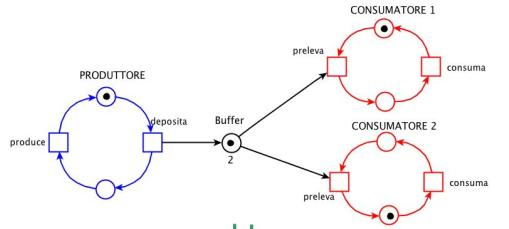
\includegraphics[scale = 0.6]{img/pt5.jpg} 
%   \end{figure}
%   Possiamo \textit{comprimere} nella stessa maniera, ottenendo, in quanto i due
%   consumatori hanno lo stesso modello di comportamento:
%   \begin{figure}[H]
%     \centering
%     \begin{tikzpicture}[node distance=2cm,bend angle=45,auto]
%       \node [place] (p0) [label=above:P2] {};
%       \node [transition] (t1) [below right of = p0, label=left:d] {};
%       \node [transition] (t2) [below left of = p0, label=left:p] {};
%       \node [place, tokens = 1] (p1) [below right of = t2, label=below:P1] {}; 
%       \node [place, tokens=1] (p3) [right of = t1, label=above:B] {};
%       \node [transition] (t4) [right of = p3, label=right:e] {};

%       \node [place, tokens=1] (p2) [above right of = t4,label=above:C1] {}; 
%       \node [transition] (t3) [below right of = p2, label=right:c] {};
%       \node [place, tokens =1] (p4) [below right of = t4, label=below:C2]
%       {}; 
      
%       \path[-{Latex[width=2mm]}]
%       (p0) edge (t1)
%       (t1) edge (p1)
%       (p1) edge (t2)
%       (t2) edge (p0)
%       (t1) edge (p3)
%       (p3) edge (t4)
%       (t4) edge (p4)
%       (p4) edge (t3)
%       (t3) edge (p2)
%       (p2) edge (t4)
%       ;
%     \end{tikzpicture}
%   \end{figure}
%   Anche qui perdo l'informazione riguardo quale dei due consumatori ha
%   effettivamente prelevato, riguardo quale dei due è pronto a \textit{prelevare}
%   e quale a \textit{consumare}, continuando ad ignorare anche la posizione
%   del buffer nei confronti della quale stanno agendo.\\
%   Si può arrivare ad avere due componenti identiche che sono concorrenti tra
%   loro. 
% \end{esempio}
% Le condizioni non sono più, in generale, booleane ma sono \textbf{posti}
% dotati di \textbf{contatori}, gli elementi all'interno sono detti
% \textbf{marche}. Ai posti si assegna anche una \textbf{capacità}. 
% \\
% Si ha inoltre che lo scatto di una transizione dipende dalla disponibilità
% delle risorse, per esempio un produttore può produrre $n$ elementi alla volta
% e il consumatore consumarne $m$. Si usano quindi archi pesati (se non indicato
% ovviamente ha peso 1, quello del normale check booleano di condizione attiva)
% tali che una transizione possa scattare sse i pesi vengono rispettati:
% \begin{figure}[H]
%   \centering
%   \begin{tikzpicture}[node distance=2cm,bend angle=45,auto]
%     \node [transition] (t0) [label=left:$t_1$] {};
%     \node [place] (p0) [above left of = t0, label=above:P0] {};       
%     \node [place, tokens = 6, minimum size = 0.9cm] (p1) [above right of = t0, label=above:P1] {}; 
%     \node [place] (p2) [below left of = t0, label=below:P2] {}; 
%     \node [place] (p3) [below of = t0, label=below:P3] {}; 
%     \node [place] (p4) [below right of = t0, label=below:P4] {}; 

%     {}; 
    
%     \path[-{Latex[width=2mm]}]
%     (p0) edge (t0)
%     (p1) edge node {5} (t0)
%     (t0) edge (p2)
%     (t0) edge node {2}(p3)
%     (t0) edge (p4)
%     ;
%   \end{tikzpicture}
%   \qquad\qquad\qquad
%   \begin{tikzpicture}[node distance=2cm,bend angle=45,auto]
%     \node [transition] (t0) [label=left:$t_1$] {};
%     \node [place, tokens = 2] (p0) [above left of = t0, label=above:P0] {};       
%     \node [place, tokens = 4, minimum size = 0.7cm] (p1) [above right of = t0, label=above:P1] {}; 
%     \node [place] (p2) [below left of = t0, label=below:P2] {}; 
%     \node [place] (p3) [below of = t0, label=below:P3] {}; 
%     \node [place] (p4) [below right of = t0, label=below:P4] {}; 

%     {}; 
    
%     \path[-{Latex[width=2mm]}]
%     (p0) edge (t0)
%     (p1) edge node {5} (t0)
%     (t0) edge (p2)
%     (t0) edge node {2}(p3)
%     (t0) edge (p4)
%     ;
%   \end{tikzpicture}
%   \caption{Esempi con la transizione $t_i$ non abilitata}
% \end{figure}
% \begin{figure}[H]
%   \centering
%   \begin{tikzpicture}[node distance=2cm,bend angle=45,auto]
%     \node [transition] (t0) [label=left:$t_1$] {};
%     \node [place, tokens = 2] (p0) [above left of = t0, label=above:P0] {};       
%     \node [place, tokens = 5, minimum size = 0.7cm] (p1) [above right of = t0, label=above:P1] {}; 
%     \node [place] (p2) [below left of = t0, label=below:P2] {}; 
%     \node [place] (p3) [below of = t0, label=below:P3] {}; 
%     \node [place] (p4) [below right of = t0, label=below:P4] {}; 

%     {}; 
    
%     \path[-{Latex[width=2mm]}]
%     (p0) edge (t0)
%     (p1) edge node {5} (t0)
%     (t0) edge (p2)
%     (t0) edge node {2}(p3)
%     (t0) edge (p4)
%     ;
%   \end{tikzpicture}
%   \qquad\qquad\qquad
%   \begin{tikzpicture}[node distance=2cm,bend angle=45,auto]
%     \node [transition] (t0) [label=left:$t_1$] {};
%     \node [place, tokens = 1] (p0) [above left of = t0, label=above:P0] {};       
%     \node [place] (p1) [above right of = t0, label=above:P1] {}; 
%     \node [place, tokens = 1] (p2) [below left of = t0, label=below:P2] {}; 
%     \node [place, tokens = 2] (p3) [below of = t0, label=below:P3] {}; 
%     \node [place, tokens = 1] (p4) [below right of = t0, label=below:P4] {}; 

%     {}; 
    
%     \path[-{Latex[width=2mm]}]
%     (p0) edge (t0)
%     (p1) edge node {5} (t0)
%     (t0) edge (p2)
%     (t0) edge node {2}(p3)
%     (t0) edge (p4)
%     ;
%   \end{tikzpicture}
%   \caption{Esempio con la transizione $t_i$ abilitata, a sinistra il ``prima''
%     e a destra il ``dopo'' lo scatto di $t_i$}
% \end{figure}
% \subsection{I Filosofi a Cena}
% Questo è un classico problema di sincronizzazione, introdotto da Dijkstra. Si ha
% un tavolo rotondo con 5 filosofi ($p_i,\,i=0,\ldots 4$), ciascuno ha davanti un
% piatto di spaghetti e si hanno solo 5 forchette ($f_i,\,i=0,\ldots 4$):
% \begin{figure}[H]
%   \centering
%   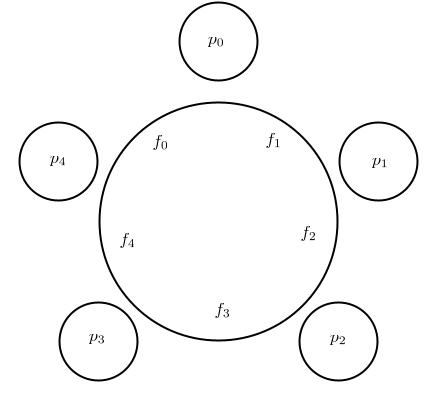
\includegraphics[scale = 0.5]{img/pt10.jpg}
%   \caption{Rappresentazione schematica del problema dei 5 filosofi}
% \end{figure}
% Ogni filosofo ha lo stesso comportamento, un po' pensa e un po' mangia,
% prendendo prima la forchetta alla sua destra e poi quella alla sua sinistra
% (perché necessitano di due forchette per mangiare). Si ha quindi il
% \textit{deadlock} se tutti vogliono mangiare, prendendo tutti in primis una
% forchetta, impedendosi tutti a vicenda di mangiare (non potendo prendere due
% forchette) o si ha la \textit{starvation} in quanto potrebbero accordarsi per
% mangiare in quattro, impedendo a uno di mangiare.\\
% Si vuole modellare tale schema. Ogni filosofo può essere modellato come una rete
% elementare, che farà da componente al modello finale:
% \begin{figure}[H]
%   \centering
%   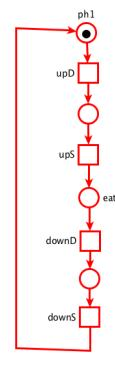
\includegraphics[scale = 0.5]{img/pt11.jpg}
% \end{figure}
% con gli eventi \textit{upD} e \textit{upS}, dove il filosofo prende la forchetta
% destra e sinistra, e rispettivamente \textit{downD} e \textit{downS}, dove le
% mette giù. Si ha la condizione che specifica che il filosofo sta pensando e
% quella che mi segnala l'azione del mangiare, oltre alle due condizioni
% intermedie che separano le azioni tra forchetta sinistra e destra.\\
% Si modella anche la componente della forchetta, con gli eventi che segnalano se
% è depositata, \textit{down}, o meno, \textit{up}:
% \begin{figure}[H]
%   \centering
%   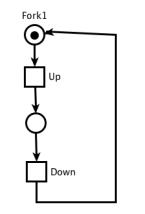
\includegraphics[scale = 0.5]{img/pt12.jpg}
% \end{figure}
% \newpage
% Combino quindi le due componenti per specificare il filosofo che prende la sua
% forchetta destra e poi la sinistra, quindi per ogni componente \textit{filosofo}
% si hanno due componenti \textit{forchetta}:
% \begin{figure}[H]
%   \centering
%   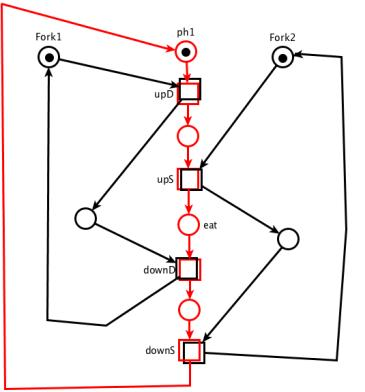
\includegraphics[scale = 0.5]{img/pt13.jpg}
% \end{figure}
% con la \textit{forchetta 1 (fork 1)} che sarà la forchetta destra e la
% \textit{forchetta 2 (fork 2)} che sarà la forchetta sinistra. Si hanno quindi
% diverse transizioni di sincronizzazione tra le due componenti (ogni volta che il
% filosofo interagisce con la forchetta).\\
% Bisogna aggiungere che ogni forchetta può essere presa da due filosofi, ognuna a
% destra di un filosofo e a sinistra di un altro:
% \begin{figure}[H]
%   \centering
%   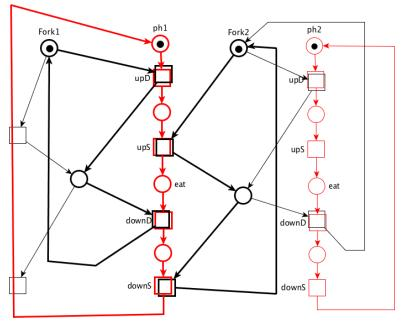
\includegraphics[scale = 0.5]{img/pt14.jpg}
% \end{figure}
% Ogni forchetta quindi si sincronizza alternativamente tra due filosofi, venendo
% presa da uno dei due filosofi. Si è arrivati quindi ad una \textbf{situazione di
%   conflitto}, o meglio ad una \textbf{situazione di confusione}.\\
% Per ora la soluzione di questo problema viene lasciato da parte per valutare il
% modello dello stesso.\\
% Si ha quindi una possibile rappresentazione del modello completo:
% \begin{figure}[H]
%   \centering
%   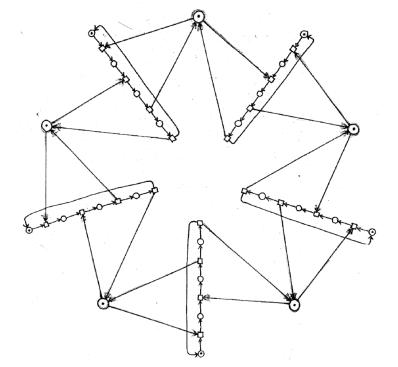
\includegraphics[scale = 0.5]{img/pt15.jpg}
% \end{figure}
% Ma ogni filosofo, come del resto ogni forchetta, si comporta nella stessa
% maniera. Si tenda quindi di \textit{ripiegare} il modello, modellando un
% un'unica componente filosofo con 5 marche distribuite nei vari stati locali del
% filosofo. Stesso discorso per le forchette. Ottengo quindi il seguente modello:
% \begin{figure}[H]
%   \centering
%   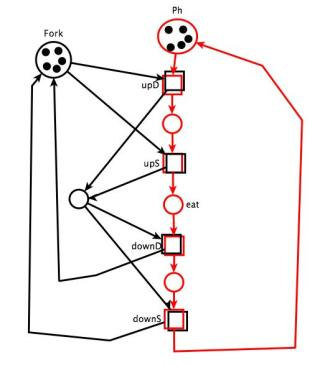
\includegraphics[scale = 0.6]{img/pt16.jpg}
% \end{figure}
% Con le due componenti, \textit{filosofo} e \textit{forchetta}, entrambe
% inizializzate con 5 marche ciascuno. Questo modello però perde informazione
% sulla forchetta che un filosofo può prendere, si ha un radicale \textbf{cambio
%   di protocollo}. Un filosofo può prendere una qualsiasi forchetta e non più
% quella alla sua destra/sinistra. Non posso quindi usare le \textit{reti Posti e
%   Transizioni} in quanto perdo troppe informazioni.\\
% L'unica soluzione possibile è quindi quella di recuperare le informazioni perse
% inserendole nelle marche, alle quali viene aggiunta una struttura dati. Si ha
% così modo di distinguere i vari filosofi e le forchette. Per compattare il
% sistema devo quindi rendere più complessa l'essenza della marca, viene
% arricchita con una struttura dati.\\
% Si arriva così ad avere una \textbf{Rete di Alto Livello}, come, per esempio,
% una \textit{rete colorata}, a partire da un rete elementare.\\
% Distinguo quindi filosofi e forchette nei due insiemi di strutture dati:
% \begin{enumerate}
%   \item $Phil=\{p_0,\ldots, p_4\}$, insieme dei filosofi
%   \item $Fork=\{f_0,\ldots, f_4\}$, insieme delle forchette
% \end{enumerate}
% Si nota che per gli indici si ha una somma \textit{modulo 5}, ovvero gli indici
% rispondono alla regola:
% \[(i+1) \mbox{ mod } 5\]
% In modo che gli indici siano ordinati avendo inoltre lo 0 che segue il 4, in
% modo circolare.\\
% Si ottiene quindi, mantenendo il protocollo iniziale:
% \begin{figure}[H]
%   \centering
%   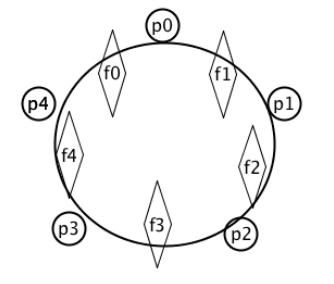
\includegraphics[scale = 0.6]{img/pt17.jpg}
% \end{figure}
% Si mantiene quindi un modello simile a quello descritto sopra ma al posto di
% marche non strutturate si ha nel posto delle 5 forchette le marche dell'insieme
% \textit{Fork} e al posto dei 5 filosofi le marche dell'insieme \textit{Phil}:
% \begin{figure}[H]
%   \centering
%   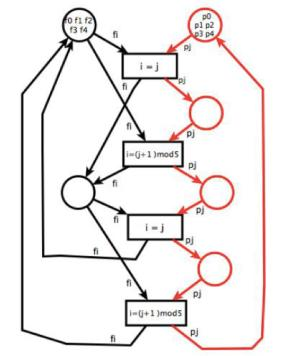
\includegraphics[scale = 0.6]{img/pt18.jpg}
% \end{figure}
% Le transizioni scattano in determinate condizioni. Per esempio la prima
% transizione, relativa al fatto che il filosofo prende la forchetta alla sua
% destra, scatta sse con l'istanza filosofo $p_j$ e forchetta $f_i$ si ha che
% $i=j$ (ho quindi almeno una forchetta, almeno un filosofo e la forchetta deve
% essere quella alla sua destra, che, per come abbiamo modellato il problema, è
% quella con lo stesso indice). Sugli archi si hanno quindi annotate determinate
% variabili che denotano istanze. Per la forchetta a sinistra si usa il modulo
% 5. Si procede quindi per i vari filosofi.
% \begin{figure}[H]
%   \centering
%   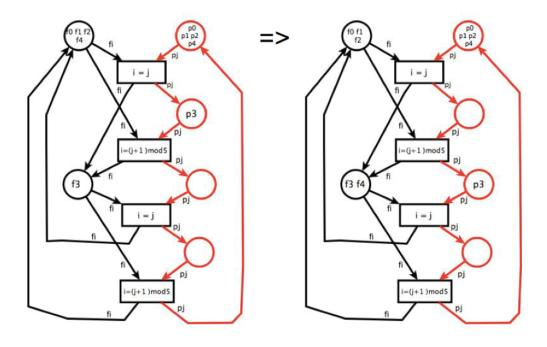
\includegraphics[scale = 0.5]{img/pt19.jpg}
%   \caption{Esempio con il filosofo $p_3$ che ha già preso la forchetta alla sua
%     destra, $f_3$, e prende quella a sinistra, $f_4$}
% \end{figure}
% \textit{Si ha quindi un prezzo per rappresentare in maniera compatta un sistema
%   elementare, mediante una rete di alto livello, ovvero l'arricchimento della
%   struttura dati}.
% \subsection{Formalizzazione delle Reti Posti e Transizioni}
% Nonostante la sezione si occupi di formalismi ci appoggiamo ad un esempio per
% avere un confronto diretto tra teoria e pratica. Questo esempio è un'n-sima
% versione del sistema produttore-consumatore, con un produttore che deposita
% a due elementi alla volta, in un buffer che ha capacità massima apri a cinque,
% che vengono consumati da due consumatori:
% \begin{figure}[H]
%   \centering
%   \begin{tikzpicture}[node distance=2cm,bend angle=45,auto]
%     \node [place, tokens = 1] (p0) [label=above:P2] {};
%     \node [transition] (t1) [below right of = p0, label=left:d] {};
%     \node [transition] (t2) [below left of = p0, label=left:p] {};
%     \node [place] (p1) [below right of = t2, label=below:P1] {}; 
%     \node [place, tokens=2] (p3) [right of = t1, label=below:$\mbox{B,
%       capacità=5}$] {}; 
%     \node [transition] (t4) [right of = p3, label=right:e] {};

%     \node [place, tokens=1] (p2) [above right of = t4,label=above:C1] {}; 
%     \node [transition] (t3) [below right of = p2, label=right:c] {};
%     \node [place, tokens = 1] (p4) [below right of = t4, label=below:C2]
%     {}; 
    
%     \path[-{Latex[width=2mm]}]
%     (p0) edge (t1)
%     (t1) edge (p1)
%     (p1) edge (t2)
%     (t2) edge (p0)
%     (t1) edge node {2} (p3)
%     (p3) edge (t4)
%     (t4) edge (p4)
%     (p4) edge (t3)
%     (t3) edge (p2)
%     (p2) edge (t4)
%     ;
%   \end{tikzpicture}
%   \caption{Modello produttore-consumatore compatto con due consumatori.}
% \end{figure}
% quindi al massimo ho cinque marche nel buffer e 2 in uno degli stati del
% consumatore (in quanto rappresenta due consumatori).\\
% Passiamo ora alla formalizzazione:

% \begin{definizione}
%   Si definisce un \textbf{sistema Posti e Transizioni (\textit{sistema P/T})} la
%   sestupla: 
%   \[\Sigma=(S,T,F,K,W;M_0)\]
%   dove:
%   \begin{itemize}
%     \item $(S,T,F)$ è una rete con:
%     \begin{itemize}
%       \item $S$ che rappresenta l'insieme dei posti
%       \item $T$ che rappresenta l'insieme delle transizioni
%       \item $F$ che rappresenta la relazione di flusso che lega posti e
%       transizioni tramite archi
%     \end{itemize}
%     \item $K:S\to\mathbb{N}^{+}\cup \{\infty\}$ che rappresenta una funzione che
%     ad ogni posto in $S$ assegna un valore, che può essere un naturale
%     strettamente positivo o anche infinito (ovvero in quel posto posso avere un
%     numero qualsiasi di marche). Il valore zero non è ammesso in quanto
%     implicherebbe che il posto non potrebbe mai essere occupato, rendendo la
%     modellazione di un tale posto inutile. $K$ è detta \textbf{funzione
%       capacità dei posti}.
%     \item $W:F\to\mathbb{N}$ che rappresenta una funzione che
%     assegna ad ogni arco un peso mediante un valore naturale che stavolta può
%     essere, oltre che infinito, anche zero. $W$ è detta \textbf{funzione peso
%       degli archi}
%     \item $M_0:S\to \mathbb{N}\cup\{\infty\}:\,\forall s\in
%     S\,\,\,M_0(s)\leq K(s)$ che rappresenta la \textbf{marcatura iniziale}
%     del sistema, ovvero una funzione che assegna ad ogni posto un naturale,
%     eventualmente nullo o infinito, minore o uguale alla capacità massima di
%     tale posto (capacità espressa dalla funzione $K$) indicante il numero di
%     marche allo stato iniziale. 
%   \end{itemize}
%   Bisogna ora definire la regola di scatto, ovvero il \textbf{gioco delle
%     marche}, la regola per cui le marche si spostano sulla rete. Si ha quindi,
%   dati:
%   \[M:S\to\mathbb{N}\cup \{\infty\}\mbox{ e }t\in T\]
%   ovvero data una marcatura e una qualsiasi transizione $t$ si ha che:
%   \[M[t>\]
%   ovvero una transizione è abilitata in una certa marcatura,
%   \begin{center}
%     sse:
%   \end{center}
%   \[\forall s\in S,\,\,M(s)\geq W(s,t)\wedge M(s)+W(t,s)\leq K(s)\]
%   ovvero per ogni posto si ha che ci sono abbastanza marche nei posti perché
%   possa scattare la transizione, ovvero c'è un arco di peso corretto che collega
%   quel posto con la transizione, avendo peso dell'arco minore o uguale al numero
%   di marche del posto, e, inoltre, si deve verificare che la transizione non
%   metta troppe marche in quel posto, quindi la marcatura del posto (ovvero il
%   numero di marche già presenti in esso) più il numero di marche che si
%   aggiungono con lo scatto della transizione non deve superare la capacità del
%   posto.
%   \begin{figure}[H]
%     \centering
%     \begin{tikzpicture}[node distance=2cm,bend angle=45,auto]
%       \node [transition] (t0) [label=left:$t_3$] {};
%       \node [transition] (t1) [left of = t0, label=left:$t_1$] {};
%       \node [transition] (t2) [right of = t0, label=right:$t_2$] {};
%       \node [place, tokens=2] (p1) [above of = t0, label=above:P1] {}; 
%       \node [place] (p2) [below of = t0, label=below:$\mbox{capacità=3}$] {}; 
      
%       \path[-{Latex[width=2mm]}]
%       (p1) edge (t1)
%       (p1) edge node {2}(t2)
%       (t1) edge (p2)
%       (t2) edge node {2}(p2)
%       (p2) edge node {3}(t0)
%       (t0) edge (p1)
%       ;
%     \end{tikzpicture}
%     %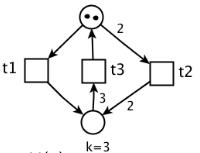
\includegraphics[scale = 0.75]{img/pt21.jpg}
%     \caption{Nell'esempio si ha che la transizione $t_2$ può scattare sse nella
%       posto precedente ho almeno due marche, in quanto l'arco tra i due ha peso
%       due. Inoltre ho il posto che segue vuoto ma con capacità massima pari a
%       tre, quindi la transizione può scattare in quanto l'arco tra i due pesa
%       due, assicurandomi che dopo la transizione, nel posto che la segue, non
%       verrà superata la capienza massima, arrivando infatti ad avere marcatura
%       pari a 2}
%   \end{figure}
%   Lo scatto della transizione, se questa è abilitata nella marcatura, mi genera
%   una nuova marcatura che viene ottenuta da quella precedente togliendo tante
%   marche dal posto che è di input alla transizione quanto il peso dell'arco che
%   connette tale posto alla transizione e aggiungendo tante marche al posto in
%   output quante il peso dell'arco che connette la transizione a tale posto,
%   ovvero, formalmente: 
%   \[M[t>M'\]
%   \begin{center}
%     sse
%   \end{center}
%   \[M[t> \wedge\, \forall s\in S,\,\,M'(s)=M(s)-W(s,t)+W(t,s)\]
%   quindi il nuovo posto avrà marcatura pari a quella precedente al più dei due
%   contributi, il primo negativo e il secondo positivo, dei pesi dei due archi.
% \end{definizione}
% \begin{definizione}
%   Dato un sistema P/T $\Sigma=(S, T , F , K , W;M_0)$ si definisce
%   l'\textbf{insieme delle marcature raggiungibili}, dalla marcatura iniziale  di
%   $\Sigma$ come:
%   \[[M_0>\]
%   ed esso è il più piccolo insieme tale che:
%   \begin{itemize}
%     \item $M_0\in [M_0>$, ovvero ola marcatura iniziale appartiene all'insieme
%     delle marcature raggiungibili
%     \item se $M\in [M_0> \wedge\,\exists t\in T:\,M[t>M'$ allora $M'\in [M_0$,
%     ovvero se $M$ appartiene all'insieme delle marcature raggiungibili ed esiste
%     una transizione una transizione tale per cui $M$ va in $M'$ allora, di
%     conseguenza si ha che $M'$ appartiene all'insieme delle marcature
%     raggiungibili dallo stato iniziale
%   \end{itemize}
%   \emph{Anche questa è una definizione per induzione}
% \end{definizione}
\chapter{Logiche temporali e model-checking}
Per capire l'importanza di questo argomento pensiamo di avere un codice
concorrente scritto in un certo linguaggio, con l'utilizzo dei \textit{thread},
con un produttore, un consumatore e un buffer. I primi due estendono la classe
\textit{thread} mentre il buffer ha i metodi \textit{synchronized} per il
prelevamento e il deposito. Questo codice simula il modello
produttore-consumatore già approfondito. Bisogna capire se questo programma
funzioni correttamente ma non posso usare le tecniche viste precedentemente per
valutare la correttezza di programmi (logica di Hoare etc$\ldots$) in quanto
abbiamo a che fare con un programma che non inizia, produce dati e finisce ma,
generalmente, si ha a che fare con un programma senza stato finale, che esegue
infinitamente le sue parti in modo concorrente. Per il modello appena ipotizzato
possiamo dire che è corretto se, ad esempio:
\begin{itemize}
  \item ogni oggetto prodotto venga prima o poi consumato
  \item nessun oggetto venga consumato più di una volta
  \item il sistema non vada in deadlock
\end{itemize}
Pensiamo ora ad una rete di Petri ``complessa'' con due processi che
condividono in un mutua esclusione una certa risorsa. Si ha quindi una sezione
critica dove un processo usa tale risorsa. Possiamo volere, per esempio, che i
due processi non siano mai contemporaneamente nella sezione critica (userebbero
insieme la risorsa) e che prima o poi un processo entri in zona critica. Un
metodo è controllare l'intero spazio delle marcature raggiungibili e verificare
che tutto vada come voluto, per la prima richiesta, ma ci sono tecniche
migliori.  \\
Un altro caso d'uso è quello dei circuiti asincroni.\\
Volendo si può adattare la logica di Hoare a modelli concorrenti ma solo se si
ha comunque un output finale e non un'evoluzione ciclica infinita. \\
Fino'ora ci si è basati sulla logica proposizionale ma tale logica ha dei
limiti, si introduce quindi la 
\textbf{logica PLTL (\textit{Propositional Linear Time Logic})} che introduce il
concetto di \textbf{tempo}, in ottica \textbf{lineare}, nel processo logico.\\
La logica PLTL viene usata per \textbf{model checking} e lo scopo generale che
ci si propone è quello di presentare un approccio formale alla progettazione e
all'implementazione di sistemi basato su un linguaggio formale che permetta di
specificarli e ragionare sulle loro proprietà. Si vogliono studiare sia sistemi
grandi, come software o addirittura sistemi operativi, che piccoli, come per
esempio una coppia di semafori. Tutti questi sistemi hanno però la medesima
caratteristica, ovvero assumono in ogni \textbf{istante di tempo} un determinato
\textbf{stato} definito dalle \textbf{variabili} del sistema stesso. Si hanno
quindi nel sistema, in ogni istante di tempo:
\begin{itemize}
  \item uno \textbf{stato}, univocamente definito dai valori delle variabili
  \item una \textbf{transizione} che segnala un passaggio da uno stato ad un
  altro
  \item una \textbf{computazione} che rappresenta una sequenza di stati di cui
  ogni coppia forma una transizione. Si introduce quindi il concetto
  \textbf{temporale} 
\end{itemize}
Il \textbf{tempo} viene pensato come un oggetto discreto, cadenzato dalle
transizioni, su cui può essere definita anche una relazione d'ordine (potrebbe
servire che un processo termini prima, dopo o nello stesso tempo di un altro).
\begin{definizione}
  Si definisce \textbf{sistema reattivo} una componente:
  \begin{itemize}
    \item non terminante e interattivo
    \item che può leggere il proprio input non solo all'inizio della
    computazione e che può produrre output non solo alla fine della sua
    computazione (si possono quindi avere multipli input e multipli output)
    \item che interagisce con altri componenti distribuiti o concorrenti
  \end{itemize}
  Sono quindi:
  \begin{itemize}
    \item sistemi concorrenti, distribuiti e asincroni
    \item Non obbediscono al paradigma input-computazione-output
    \item non si possono analizzare con gli strumenti della logica di Hoare
  \end{itemize}
  avendo come esempi di comportamento:
  \begin{itemize}
    \item ``se un messaggio è stato spedito, prima o poi sarà consegnato al
    destinatario''
    \item ``La spia d’allarme resta accesa fino a quando il dispositivo viene
    spento'' 
    \item ``a partire da qualsiasi stato è possibile riportare il sistema allo
    stato iniziale''
  \end{itemize}
\end{definizione}
Bisogna stabilire la correttezza di un sistema reattivo esprimendo il criterio
di correttezza come formula di un opportuno linguaggio logico. Il sistema
reattivo si modella tramite un sistema di transizioni, tramite i \textbf{modelli
di Kripke}, e valutiamo se la formula è vera nel sistema di transizioni, tramite
logiche temporali e algoritmi specifici.\\
Si hanno sistemi non terminanti che usano un numero \textbf{finito} di
variabili e di conseguenza si ha un numero di stati, in cui transita il sistema,
\textbf{finito}. Si hanno infatti sistemi di transizione finiti che
\textit{``comprimono''} sistemi non terminanti, con computazioni di lunghezza
infinita, in una rappresentazione finita.
Si ricorda che si possono inoltre categorizzare le proprietà che vogliamo
specificare come: 
\begin{itemize}
  \item \textbf{proprietà di safety}
  \item \textbf{proprietà di liveness}
  \item \textbf{proprietà di fairness}
\end{itemize}
Introduciamo quindi meglio i \textbf{modelli di Kripke}.\\
\begin{definizione}
  Definiamo un \textbf{sistema di transizioni} $A$ come:
  \[A=(Q,T)\]
  con:
  \begin{itemize}
    \item $Q$ come insieme di stati (potrebbe essere infinito ma studieremo i
    casi finiti)
    \item $T\subseteq Q\times Q$ insieme delle transizioni di stato che portano
    da uno stato ad un altro
  \end{itemize}
\end{definizione}
\begin{definizione}
  Definiamo \textbf{cammino} come:
  \[\pi=q_0q_1q_2\ldots,\,\,\,q_i\in T,\,\,\, \forall\,i\]
  Un cammino può essere infinito.\\
  Definiamo \textbf{cammino massimale} un cammino che non può più essere esteso
  (generalmente studieremo casi dove i cammini massimali sono infiniti).
\end{definizione}
\begin{definizione}
  Definiamo un \textbf{modello di Kripke} $A$ come un sistema di transazioni a
  cui ad ogni stato è associato, dato l'insieme delle proposizioni atomiche
  $AP=\{z_1,z_2,\ldots z_n\}$, un insieme  di
  proposizioni atomiche che sono vere in quello stato:
  \[A=(Q,T,I)\]
  avendo una \textbf{funzione di interpretazione} $I$, che mi restituisce
  l'insieme delle proposizioni atomiche vere in uno stato, tale che:
  \[I:Q\to 2^{AP}\]
  Potrei avere stati dove nessuna proposizione atomica è vera avendo il
  sottoinsieme associato vuoto.\\
  NOn si specifica di base uno stato iniziale ma si può arricchire la
  definizione con uno stato iniziale.
\end{definizione}
\begin{esempio}
  Vediamo un esempio:
  \begin{figure}[H]
    \centering
    \begin{tikzpicture}[node distance=2.5cm,bend angle=45,auto]
      \node [place] (p0) [label=below left:q] {1};
      \node [place] (p1) [right of = p0, label=below left:q] {2};
      \node [place] (p2) [right of = p1, label=below left:p] {5};
      \node [place] (p3) [below of = p0, label=below left:{p,r}] {4}; 
      \node [place] (p4) [below of = p1, label=below left:{p,q}] {3}; 
      \node [place] (p5) [below of = p2, label=below left:{p,r}] {6}; 
      \path[-{Latex[width=2mm]}]
      (p0) edge (p1)
      (p1) edge (p2)
      (p1) edge (p4)
      (p4) edge (p3)
      (p3) edge (p0)
      (p2) edge [bend left= 25](p5)
      (p5) edge [bend left= 25](p2)
      ;
    \end{tikzpicture}
  \end{figure}
  Dove:
  \begin{itemize}
    \item $AP=\{p, q, r\}$, insieme delle proposizioni atomiche
    \item $Q=\{1,2,3,4,5,6\}$, insieme degli stati
    \item $T=\{(1,2),(2,3),(2,5),(5,6),(6,5),\cdots\}$, insieme delle
    transizioni 
    \item $I(4) =\{p, r\}$, $I(2) =\{q\}$ etc$\ldots$, gli altri sono indicati
    in basso a sinistra di ogni stato
    \item $1,2,5$ è un cammino non massimale
    \item $1,2,5,6,\overline{5,6}$ è un cammino massimale (qui indico con la
    linea sopra gli stati in cui poi si continua a ciclare)
    \item $1,2,3,4,\overline{1,2,3,4}$ è un cammino massimale
    \item $1,2,3,4,1,2,5,6\overline{5,6}$ è un cammino massimale
  \end{itemize}
\end{esempio}
Si può quindi già intuire che:
\begin{center}
  \textit{le logiche temporali sono frammenti della logica del primo ordine}
\end{center}
Infatti con le logiche temporali, come la \textit{logica PLTL}, si supera il
limite di rappresentazione temporale della logica proposizionale, permettendo,
per esempio, di rappresentare proposizioni del tipo \textit{``prima o poi'',
  ``accade sempre che'' etc$\ldots$}.\\
Si ha un \textbf{tempo lineare e discreto}, che si può pensare di rappresentare
nella logica classica proposizionale (per esempio come indice) ma questo
comporta il doversi dotare di infinite variabili proposizionali (corrispondenti
ad ogni \textit{``step''} temporale) e comporta l'ottenimento di una formula
proposizionale di lunghezza infinita. Si può pensare di passare allo studio di
questi casi con la \textit{logica predicativa} ma sarebbe ben più del
necessario, in quanto le procedure sarebbero di complessità molto elevata, a
causa della grande espressività della logica predicativa. Inoltre la logica dei
predicati è indecidibile. \\
Si cerca quindi la via di mezzo cercando logiche specializzate, meno espressive
della logica predicativa ma decidibili rispetto ai problemi presi in
considerazione. Si cerca una logica con procedure efficienti rispetto
all'ampiezza della descrizione del problema in analisi (ovvero tipicamente
l'ampiezza del sistema di transizioni), che è direttamente proporzionale al
numero di stati del sistema (lineare rispetto al numero degli stati), e rispetto
alla lunghezza della formula che esprime la proprietà da testare.

\subsection{Sintassi}
Vediamo innanzitutto la \textbf{sintassi} della logica PLTL che chiamiamo anche
LTL.\\
Si ha a che fare con un \textit{vocabolario} più ampio rispetto a quelli della
logica proposizionale, vengono infatti aggiunti dei \textbf{connettivi} utili
alla rappresentazione temporale richiesta.
\begin{definizione}
  Nella logica PLTL, oltre ai connettivi logici classici della logica
  proporzionale, si definiscono i seguenti connettivi:
  \begin{itemize}
    \item \textbf{X}, detto anche \textbf{next} o \textbf{tomorrow}. È un
    connettivo unario e viene rappresentato con $\circ$
    \item \textbf{F}, detto anche \textbf{sometime} o \textbf{future}. È un
    connettivo unario e viene rappresentato con $\diamond$
    \item \textbf{G}, detto anche \textbf{globally} o \textbf{always}. È un
    connettivo unario e viene rappresentato con $\square$
    \item \textbf{U}, detto anche \textbf{until}. È un connettivo binario
  \end{itemize}
  Viene inoltre indicato con $V$ l'\textbf{insieme delle variabili
    proposizionali}, l'\textbf{insieme delle proposizioni atomiche},
  variabili che hanno lo stesso significato della logica
  proposizionale, quindi ogni variabile corrisponde ad una singola proposizione
  del linguaggio naturale. 
\end{definizione}
\textbf{Qui chiamo $V$ quello che prima chiamavo $AP$ per non dover riscrivere
  tutti gli appunti tratti da metodi formali.\\}
\begin{definizione}
  Diamo ora una definizione, formale, procedendo per induzione di
  \textbf{formula ben formata} del linguaggio PLTL (definendo così l'aspetto
  sintattico della logica PLTL): 
  \begin{itemize}
    \item $\forall p\in V$ vale che $p$ è una formula del linguaggio PLTL,
    ovvero le variabili proposizionali della logica classica sono formule del
    linguaggio PLTL. Questa è una \emph{formula atomica}
    \item i simboli $\top$ (detto anche \emph{true} che semanticamente
    semplifica
    una tautologia) e $\bot$ (detto anche \textit{false} o \emph{bottom} che
    semanticamente specifica una formula sempre falsa, ovvero una
    contraddizione) sono formule del linguaggio PLTL. Anche questa è una
    \emph{formula atomica}
    \item se $A$ è una formula del linguaggio PLTL allora lo sono anche:
    \begin{itemize}[label=$\ast$]
      \item $\neg A$
      \item $\mathbf{X}A$
      \item $\mathbf{F}A$
      \item $\mathbf{G}A$
    \end{itemize}
   
    \item  se $A$ e $B$ sono formule del linguaggio PLTL allora lo sono anche:
    \begin{itemize}[label=$\ast$]
      \item $A\to B$
      \item $A\land B$
      \item $A\lor B$
      \item $A\mathbf{U}B$ (anche $\mathbf{U}(A,B)$)
    \end{itemize}
    \item nient'altro appartiene all'insieme delle formule del linguaggio PLTL
  \end{itemize}
  Quindi si nota come \textbf{l'insieme delle formule PLTL contiene quello delle
    formule classiche della logica proporzionale}. Si ha quindi che l'insieme
  delle formule PLTL non è altro che un'estensione di quello delle formule
  classiche della logica proposizionale.
\end{definizione}
Si hanno varianti della logica temporale con anche operatori relativi al passato
ma non sono utili in merito al model checking.
\begin{definizione}
  La sintassi delle formule del linguaggio PLTL possono essere definite usando
  anche la notazione \textbf{BNF (Backus-Naur Form o Backus Normal Form)},
  ovvero, $\forall p\in V$:
  \[A::=p\,|\,\top\,|\,\bot\,|\,(\neg A)\,|\,(A\land A)\,|\,(A\lor A)\,|\,(A\to
    A)\,|\,(\mathbf{X}A)\,|\,(\mathbf{F}A)\,|\,(\mathbf{G}A)\,|\,(A\mathbf{U}A)
  \] 
  Non si è usata quindi una definizione ricorsiva ma viene invece usata una
  \textbf{grammatica}\\
  \begin{shaded}
    La BNF (Backus-Naur Form o Backus Normal Form) è una metasintassi, ovvero un
    formalismo attraverso cui è possibile descrivere la sintassi di linguaggi
    formali (il prefisso meta ha proprio a che vedere con la natura circolare di
    questa definizione). Si tratta di uno strumento molto usato per descrivere
    in modo preciso e non ambiguo la sintassi dei linguaggi di programmazione,
    dei protocolli di rete e così via, benché non manchino in letteratura esempi
    di sue applicazioni a contesti anche non informatici e addirittura non
    tecnologici. La BNF viene usata nella maggior parte dei testi sulla teoria
    dei linguaggi di programmazione e in molti testi introduttivi su specifici
    linguaggi. \\
    In termini formali, la BNF può essere vista come un formalismo per descrivere
    grammatiche libere dal contesto.  \\
    Una specifica BNF è un insieme di regole di derivazione ciascuna espressa
    nella forma: 
    \begin{center}
      \textit{<simbolo> ::= \_espressione\_}
    \end{center}
  \end{shaded}
\end{definizione}
Il cammino nel modello di Kripke corrisponde ad una esecuzione di un sistema,
che è una sequenza di stati. 
\subsection{Semantica}
\begin{definizione}
  La \textbf{semantica}, ovvero il significato dei connettivi della logica PLTL,
  è data usando i cosiddetti \textbf{modelli lineari} (si ricorda l'uso di un
  tempo lineare).\\
  Si consideri una struttura algebrica di questo tipo:
  \[M=\langle S,\,\rho, \,\to, \,\Vdash\rangle\]
  dove:
  \begin{itemize}
    \item $S$ è un \textbf{insieme infinito di stati}, detti anche
    \textbf{mondi}
    \item $\rho \in S$ è uno stato del modello detto anche \textbf{root} o
    \textbf{radice}. In tale stato viene codificato il \textbf{tempo zero}
    \item $\to$ è una relazione binaria su $S$ detta \textbf{relazione di
      transizione} la quale introduce un \textbf{ordinamento lineare} sugli
    elementi di $S$. Si ha quindi che:
    \[\to\,\subseteq S\times S\]
    e, $\forall \alpha \in S$, \textbf{esiste ed è unico} $\beta\in S$ tale che
    vale:
    \[\alpha\to\beta\]
    Preso quindi uno stato qualsiasi ho un solo modo per passare ad un altro
    stato (esiste quindi un ``prima'' e un ``dopo'').\\
    Inoltre vale che, $\forall \alpha\in S$, $\alpha\not\to \rho$, dove $\rho\in
    S$ è l'unico elemento di $S$ a godere di questa proprietà (in quanto $\rho$
    codifica il tempo zero). 
    \item $\Vdash$ è una relazione binaria, inclusa in $S\times V$, detta
    \textbf{relazione di soddisfacibilità}. Solitamente con $\alpha\Vdash p$
    si indica che $(\alpha,p)\in\,\Vdash$ è valido, ovvero che $\alpha$
    \textbf{soddisfa} $p$, con $\alpha\in S$ e $p\in V$
  \end{itemize}
  La struttura $M$ viene detta \textbf{modello per PLTL}.\\
  Si nota come questi modelli lineari seguano un ordinamento simile a quello che
  si ha tra i numeri in $\mathbb{N}$.\\ 
  Si nota come la semantica della logica PLTL sia drasticamente più complessa
  di quella della logica classica proposizionale 
\end{definizione}
\newpage
Bisogna dare ora significato ai connettivi PLTL. Per i connettivi della logica
proposizionale si usano tavole di verità e induzione ma per la logica PLTL le
cose sono un po' diverse.\\
Per dare un significato alle formule del linguaggio PLTL bisogna basarsi sui
modelli per PLTL.\\

\begin{definizione}
  Siano:
  \begin{itemize}
    \item $M=\langle S,\,\rho, \,\to, \,\Vdash\rangle$ un modello per PLTL
    \item $\alpha\in S$ uno stato
    \item $A$ una formula del linguaggio PLTL
  \end{itemize}
  si ha che la \textbf{soddisfacibilità} di $A$ nello stato $\alpha$ di $M$
  viene indicata con:
  \[(M,\alpha)\Vdash A\]
  e tale soddisfacibilità (o verità) della formula $A$ viene definita per
  induzione sulla struttura di $A$.\\
  Diciamo anche che un a formula è vera rispetto ad uno stato $q$ del modello di
  Kripke se è vera in tutti i cammini massimali $\pi$ che partono da $q$,
  dicendo che la formula $\alpha$ è soddisfatta in $\pi$, ovvero $\alpha\vDash
  \pi$.\\
  Per comodità indichiamo un cammino massimale generico con:
  \[\pi=q_0q_1\ldots q_n\]
  e un suffisso di ordine $i$:
   \[\pi^{(i)}=q_iq_{i+1}\ldots q_j,\mbox{ avendo }\pi=\pi^{(i)}\]
  Si ha quindi: 
  \begin{enumerate}
    \item se $A$ è una variabile proposizionale allora vale $(M,\alpha)\Vdash A$
    sse $\alpha\Vdash A$ per la relazione $\Vdash$ definita da $M$. Questo è un
    \textbf{caso base}
    \item se $A$ è $\top$ allora vale $(M,\alpha)\Vdash\top$, ovvero il true è
    \textbf{soddisfatto} o \textbf{forzato} ovunque. Il simbolo \emph{true} è
    vero in ogni stato e in ogni modello (siamo nel concetto di tautologia).
    Questo è un \textbf{caso base}
    \item se $A$ è $\bot$ allora vale $(M,\alpha)\nVdash\bot$, ovvero il false
    non è mai soddisfatto qualsiasi sia lo stato. Questo è un \textbf{caso base}
    \item se $A$ è $B\land C$ (con $B$ e $C$ formule PLTL) allora vale
    $(M,\alpha)\Vdash B\land C$ sse $(M,\alpha)\Vdash B$ e $(M,\alpha)\Vdash C$
    \item se $A$ è $B\lor C$ (con $B$ e $C$ formule PLTL) allora vale
    $(M,\alpha)\Vdash B\lor C$ sse $(M,\alpha)\Vdash B$ oppure $(M,\alpha)\Vdash
    C$ 
    \item se $A$ è $B\to C$ (con $B$ e $C$ formule PLTL) allora vale\\
    $(M,\alpha)\Vdash B\to C$ sse $(M,\alpha)\nVdash B$ oppure $(M,\alpha)\Vdash
    C$ 
    \item se $A$ è $\neg B$ (con $B$ formula PLTL) allora vale
    $(M,\alpha)\Vdash\neg B$ sse vale $(M,\alpha)\nVdash B$
    \item se $A$ è del tipo $\mathbf{X}\,B$ allora vale $(M,\alpha)\Vdash
    \mathbf{X}\,B$ sse vale $(M,\beta)\Vdash B$ (ovvero quando $B$ è soddisfatto
    nello stato $\beta$ di M), dove $\beta\in S$ è lo stato
    successivo (nonché unico) ad $\alpha$, ovvero si ha $\alpha\to\beta$
    \item se $A$ è del tipo $\mathbf{F}\,B$ allora vale $(M,\alpha)\Vdash
    \mathbf{F}\,B$ sse esiste una sequenza finita
    $\alpha_0\to\alpha_1\to\ldots\to\alpha_n$, con $\alpha=\alpha_0$ e $n\geq
    0$, tale che $(M,\alpha_n)\Vdash B$ (ovvero sse esiste un punto ``nel
    futuro'', ovvero $alpha_n$, che però potrebbe anche essere $\alpha_0$, dove
    la formula $B$ è soddisfatta)
    \item se $A$ è del tipo $B\,\mathbf{U}\,C$ allora vale $(M,\alpha)\Vdash
    B\,\mathbf{U}\,C$ sse esiste una sequenza finita
    $\alpha_0\to\alpha_1\to\ldots\to\alpha_n$, con $\alpha=\alpha_0$ e $n\geq
    0$, tale che $(M,\alpha_n)\Vdash C$ e tale che $(M,\alpha_i)\Vdash
    B,\,\,\,i=0,1,\ldots,n-1$ (ovvero deve esistere uno stato ``nel futuro'' di
    $\alpha$ che soddisfa $C$ e ogni stato intermedio a quello che soddisfa $C$
    deve soddisfare $B$) 
    \item se $A$ è del tipo $\mathbf{G}\,B$ allora vale $(M,\alpha)\Vdash
    \mathbf{G}\,B$ sse $(M,\alpha)\Vdash B$ e $(M,\beta)\Vdash \mathbf{G}\,B$
    dove $\beta\in S$ è lo stato successivo (nonché unico) ad $\alpha$, ovvero
    si ha $\alpha\to\beta$ (ovvero sse nello stato $\alpha$ è soddisfatto $B$ e
    nello stato $\beta$ è soddisfatto $\mathbf{G}\,B$). Questa è una definizione
    ricorsiva (anche se uso $\mathbf{G}\,B$ su uno stato successivo ad
    $\alpha$)
  \end{enumerate}
  I primi 3 punti sono i casi base, quelli successivi sono i passi induttivi.\\
  I primi 7 punti sono simili a quelli della logica proposizionale, se ci
  limitiamo ad un solo mondo
\end{definizione}
\textbf{Vedere anche esempio su slide.\\}
\begin{esempio}
  Graficamente si ha qualcosa del tipo:
  \begin{figure}[H]
    \centering
    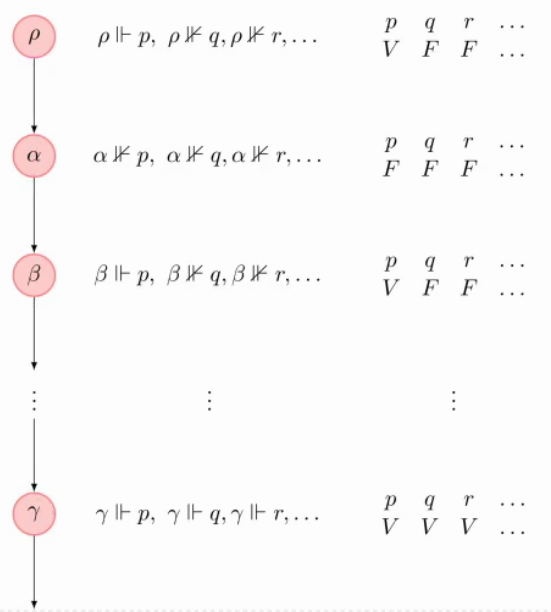
\includegraphics[scale = 0.263]{img/pltl.png}
  \end{figure}
  \textbf{che prosegue infinitamente}. Si nota che in ogni stato si specifica se
  una variabile proposizionale (che sono infinite) è soddisfatta e, per ciascuna
  variabile, si definisce una sorta di \textit{tabella di verità}, che
  specificare la soddisfacibilità di una variabile in un determinato stato
\end{esempio}
Si nota che la definizione di \textbf{modello PLTL} non esclude che due stati
diversi possano soddisfare le stesse variabili, ovvero che si possano comportare
nello stesso modo \textit{(come se nulla cambiasse nel tempo)}.

\end{document}
% LocalWords:  Machine Learning dell multicore monocore checking mutex thread
% LocalWords:  race condition graph sottoprocessi Petri Morgan int const while
% LocalWords:  if return ht primis postcondizione Hoare then endif for endwhile
% LocalWords:  endfor program counter skip and not cccccc ccccc derivabilità of
% LocalWords:  weakest precondition sse step repeat until endrepeat array java
% LocalWords:  modelling contract programming Eiffel assert language Calculus
% LocalWords:  postcondizioni denotazionali Calculus of Communicating Systems
% LocalWords:  Communicating Systems CCS composizionalità Milner communicating
% LocalWords:  sequential CSP transputer hand shacking process processes System
% LocalWords:  Pnueli Harvel sottoprocesso all deadlock Labeled Transition LTS
% LocalWords:  bisimulazione sender ossrvabile  Nil rietichettatura concurrency
% LocalWords:  rinominazione true LocalWords bisimili bisimilitudine bisimile
% LocalWords:  rietichettato interleaving handshaking estensionalità
% LocalWords:  l'unfolding
